%================================================
\chapter{Fundamentos ecológicos do nicho}
%================================================

\begin{chapteropening}
	
	A distribuição geográfica das espécies constitui um dos temas centrais da Ecologia, da Biogeografia e das Ciências da Conservação. Desde os trabalhos pioneiros de Charles Darwin e Alfred Russel Wallace, pesquisadores buscam compreender por que determinadas espécies ocorrem em algumas regiões do planeta, enquanto estão ausentes de outras aparentemente semelhantes.
	
	Essa questão tornou-se ainda mais relevante diante dos desafios contemporâneos associados às mudanças climáticas globais, à perda de habitats, às invasões biológicas e à necessidade de planejar estratégias eficientes de conservação da biodiversidade. Em todos esses contextos, compreender os fatores que limitam ou favorecem a ocorrência das espécies é um passo fundamental para prever como populações e ecossistemas poderão responder às transformações ambientais em curso.
	
	A Modelagem de Distribuição de Espécies (\textit{Species Distribution Modeling} -- SDM) surge como uma poderosa ferramenta para investigar essas questões. Entretanto, antes de compreender algoritmos, métricas de desempenho, projeções climáticas ou técnicas computacionais, é necessário compreender os fundamentos ecológicos que sustentam essas abordagens.
	
	Toda modelagem de distribuição é, essencialmente, uma hipótese ecológica sobre a relação entre organismos e ambiente. Quando um modelo estima que determinada região apresenta alta adequabilidade para uma espécie, ele está implicitamente assumindo que certos conjuntos de condições ambientais favorecem a sobrevivência, o crescimento e a persistência dessa espécie ao longo do tempo. Em outras palavras, os modelos procuram representar matematicamente aspectos do nicho ecológico.
	
	Nesta unidade serão apresentados os principais conceitos que fundamentam a Modelagem de Distribuição de Espécies. Serão discutidas a evolução histórica do conceito de nicho ecológico, as contribuições de Grinnell, Elton e Hutchinson, a distinção entre nicho fundamental e nicho realizado, as diferenças entre distribuição observada e distribuição potencial, além da importância da conservação de nicho para projeções sob mudanças climáticas.
	
	Ao final da unidade, o leitor compreenderá que os modelos de distribuição não são apenas algoritmos estatísticos aplicados a mapas ambientais, mas representações simplificadas de processos ecológicos complexos que conectam organismos, ambiente e espaço geográfico.
	
\end{chapteropening}

\begin{objetivos}
	Ao final desta unidade, o estudante deverá ser capaz de:
	
	\begin{itemize}
		
		\item compreender a importância do conceito de nicho ecológico como fundamento teórico da Modelagem de Distribuição de Espécies;
		
		\item reconhecer a distribuição geográfica das espécies como resultado da interação entre fatores abióticos, fatores bióticos e processos históricos de dispersão;
		
		\item diferenciar as principais interpretações históricas do nicho ecológico propostas por Grinnell, Elton e Hutchinson;
		
		\item compreender a distinção entre nicho fundamental, nicho realizado e distribuição potencial;
		
		\item interpretar criticamente a relação entre espaço geográfico e espaço ambiental;
		
		\item compreender o papel do BAM framework na delimitação dos processos que controlam a distribuição das espécies;
		
		\item diferenciar distribuição observada, distribuição real e distribuição modelada;
		
		\item compreender a hipótese de conservação de nicho e suas implicações para projeções espaciais e temporais;
		
		\item interpretar estudos de Modelagem de Distribuição de Espécies à luz dos fundamentos ecológicos que sustentam suas inferências;
		
		\item relacionar os conceitos teóricos apresentados com um estudo de caso real utilizando a espécie amazônica \textit{Dinizia excelsa} Ducke.
		
	\end{itemize}
	
\end{objetivos}

%================================================
\section{Por que toda SDM começa com uma hipótese ecológica?}
%================================================

A crescente popularização dos Sistemas de Informação Geográfica (SIG), dos bancos de dados globais de biodiversidade e dos algoritmos de aprendizado de máquina tornou a Modelagem de Distribuição de Espécies uma das abordagens mais utilizadas na Ecologia contemporânea. Atualmente, pesquisadores podem obter milhares de registros de ocorrência por meio de plataformas como GBIF, SpeciesLink e iNaturalist, acessar dezenas de variáveis ambientais globais e ajustar modelos complexos utilizando poucas linhas de código em linguagens como R ou Python.

Embora esses avanços tenham ampliado significativamente a acessibilidade das técnicas de modelagem, eles também criaram um risco importante: a falsa percepção de que a Modelagem de Distribuição de Espécies é apenas um procedimento computacional ou estatístico.

Na realidade, nenhum modelo de distribuição possui significado ecológico sem uma hipótese biológica que justifique as relações observadas entre espécies e ambiente. Antes de selecionar algoritmos, métricas de avaliação ou cenários climáticos futuros, o pesquisador precisa responder uma pergunta fundamental:

\begin{quote}
	\textit{Quais processos ecológicos explicam a ocorrência desta espécie nos locais onde ela é observada?}
\end{quote}

Essa questão está no centro da Ecologia desde o século XIX e permanece como um dos principais desafios da ciência ecológica moderna. A distribuição das espécies não é aleatória. Organismos ocorrem em determinados locais porque esses locais oferecem condições ambientais compatíveis com suas exigências fisiológicas, ecológicas e evolutivas. Ao mesmo tempo, muitas regiões potencialmente adequadas permanecem desocupadas devido a limitações de dispersão, barreiras geográficas, eventos históricos ou interações ecológicas desfavoráveis.

Consequentemente, toda Modelagem de Distribuição de Espécies representa uma tentativa de inferir os mecanismos que conectam organismos ao ambiente. Os modelos utilizam padrões espaciais observados para estimar quais condições ambientais estão associadas à presença da espécie e, posteriormente, projetam essas relações para outras regiões ou períodos temporais.

Essa lógica está intimamente relacionada ao conceito de nicho ecológico. Quando um modelo relaciona ocorrências de uma espécie à temperatura, precipitação, altitude ou características do solo, ele está assumindo que essas variáveis representam componentes importantes do nicho da espécie. O objetivo do modelo é identificar a porção do espaço ambiental que apresenta condições semelhantes àquelas observadas nos locais onde a espécie ocorre.

Nesse contexto, os algoritmos não constituem o elemento central da modelagem. Diferentes métodos, como GLM, GAM, Random Forest, Boosted Regression Trees ou Maxent, representam apenas estratégias matemáticas distintas para estimar uma mesma relação ecológica subjacente. O fundamento biológico permanece o mesmo: compreender como os organismos respondem aos gradientes ambientais que estruturam sua distribuição geográfica.

Essa perspectiva é amplamente defendida por autores como \textcite{guisan2005predicting}, \textcite{elith2009}, \textcite{peterson2011}, \textcite{franklin2010} e \textcite{guisan2017habitat}, que enfatizam que modelos de distribuição devem ser interpretados como hipóteses ecológicas explícitas e não apenas como ferramentas preditivas.

A importância dessa visão torna-se ainda mais evidente quando modelos são utilizados para apoiar decisões de conservação. Áreas prioritárias para conservação, projeções de impactos climáticos, identificação de refúgios ambientais e avaliação do potencial invasivo de espécies dependem diretamente da validade ecológica das relações estimadas pelos modelos. Se as hipóteses ecológicas forem inadequadas, mesmo algoritmos estatisticamente sofisticados poderão produzir inferências equivocadas.

Por essa razão, compreender os fundamentos ecológicos do nicho constitui o primeiro passo para qualquer estudo de Modelagem de Distribuição de Espécies. Antes de aprender como construir modelos, é necessário compreender o que os modelos representam, quais processos ecológicos tentam capturar e quais limitações estão associadas às suas inferências.

Nos tópicos seguintes será apresentada a evolução histórica do conceito de nicho ecológico e como diferentes interpretações desse conceito contribuíram para a construção da moderna Modelagem de Distribuição de Espécies.

%================================================
\section{A distribuição das espécies como problema central da Ecologia}
%================================================

Compreender por que as espécies ocorrem em determinados locais e estão ausentes de outros constitui uma das questões mais antigas e fundamentais da Ecologia. Muito antes do desenvolvimento dos computadores, dos Sistemas de Informação Geográfica (SIG) ou da Modelagem de Distribuição de Espécies, naturalistas já buscavam explicar os padrões espaciais da biodiversidade observados em diferentes regiões do planeta.

Durante as grandes expedições científicas dos séculos XVIII e XIX, exploradores como Alexander von Humboldt, Charles Darwin e Alfred Russel Wallace observaram que a composição das comunidades biológicas variava sistematicamente ao longo de gradientes geográficos e ambientais. Espécies encontradas em determinadas regiões frequentemente estavam ausentes em áreas aparentemente semelhantes, enquanto outras apresentavam distribuições restritas a ambientes específicos. Essas observações levaram ao surgimento de uma questão fundamental:

\begin{quote}
	\textit{Quais fatores determinam onde uma espécie pode ou não ocorrer?}
\end{quote}

A resposta para essa pergunta tornou-se um dos principais objetivos da Ecologia, da Biogeografia e, mais recentemente, da Modelagem de Distribuição de Espécies.

Historicamente, diferentes explicações foram propostas para compreender os padrões de distribuição geográfica dos organismos. Algumas enfatizavam a influência das condições ambientais, como temperatura, precipitação e disponibilidade de recursos. Outras destacavam a importância das interações ecológicas, da competição entre espécies, da predação, do mutualismo e das limitações impostas pela dispersão. Posteriormente, fatores evolutivos e históricos também passaram a ser reconhecidos como elementos fundamentais para compreender a distribuição atual da biodiversidade.

Atualmente, existe amplo consenso de que a distribuição geográfica das espécies resulta da interação entre múltiplos processos ecológicos e evolutivos que operam simultaneamente em diferentes escalas espaciais e temporais \parencite{brown1995,wiens2011,franklin2010,guisan2017habitat}.

Em escala global, os grandes gradientes climáticos exercem forte influência sobre os limites de distribuição das espécies. Regiões tropicais, temperadas, boreais e áridas apresentam conjuntos distintos de condições ambientais que selecionam organismos capazes de sobreviver sob essas circunstâncias. Temperatura, precipitação, radiação solar, sazonalidade climática e disponibilidade hídrica figuram entre os principais filtros ambientais responsáveis pela organização da biodiversidade em escala planetária.

Em escalas regionais, fatores como relevo, hidrologia, características do solo, heterogeneidade ambiental e conectividade da paisagem tornam-se progressivamente mais importantes. Já em escalas locais, interações ecológicas diretas, como competição, herbivoria, predação, facilitação e mutualismos, frequentemente exercem influência decisiva sobre a presença ou ausência das espécies.

Esse conjunto hierárquico de processos é frequentemente representado pelo conceito de filtros ecológicos. Segundo essa perspectiva, a distribuição observada de uma espécie resulta da passagem sucessiva por diferentes filtros que restringem sua ocorrência potencial.

Inicialmente, os organismos precisam apresentar características fisiológicas compatíveis com as condições ambientais disponíveis. Em seguida, precisam ser capazes de alcançar a área por meio de processos de dispersão. Finalmente, devem conseguir persistir localmente em meio às interações ecológicas existentes na comunidade.

Essa lógica pode ser visualizada como uma sequência de restrições progressivas:

\begin{center}
	Condições ambientais adequadas
	$\rightarrow$
	Capacidade de dispersão
	$\rightarrow$
	Interações ecológicas compatíveis
	$\rightarrow$
	Persistência local
\end{center}

Em outras palavras, uma espécie não ocorre em determinado local apenas porque o ambiente é adequado. Ela também precisa ter alcançado esse local ao longo de sua história evolutiva e ser capaz de coexistir com os demais organismos presentes.

Essa visão integradora foi formalizada por diversos autores ao longo das últimas décadas e constitui a base conceitual da moderna biogeografia ecológica \parencite{soberon2005,soberon2007,soberon2009,barve2011crucial}.

A importância dessa discussão para a Modelagem de Distribuição de Espécies é direta. Quando utilizamos registros de ocorrência e variáveis ambientais para ajustar um modelo, estamos tentando identificar quais componentes desse conjunto de filtros ecológicos estão representados nos dados disponíveis.

Na maioria dos casos, os modelos correlativos tradicionais utilizam predominantemente informações relacionadas aos filtros ambientais. Variáveis climáticas, topográficas e edáficas funcionam como aproximações dos fatores que limitam fisiologicamente a ocorrência das espécies. Entretanto, os modelos raramente incorporam explicitamente todos os processos responsáveis pela distribuição observada, especialmente aqueles relacionados às interações ecológicas e à história biogeográfica.

Essa limitação não reduz a utilidade dos modelos, mas exige que suas interpretações sejam realizadas de forma biologicamente consistente. Um mapa de adequabilidade ambiental não representa diretamente a probabilidade de ocorrência de uma espécie nem sua abundância populacional. O que ele representa é uma estimativa das condições ambientais associadas às ocorrências utilizadas na calibração do modelo.

Por essa razão, compreender os mecanismos ecológicos que estruturam a distribuição das espécies é fundamental para interpretar corretamente os resultados produzidos por SDM. Os algoritmos podem identificar padrões espaciais complexos, mas a interpretação ecológica desses padrões depende do conhecimento dos processos que governam a distribuição dos organismos na natureza.

Nas últimas décadas, essa compreensão tornou-se ainda mais importante diante das mudanças climáticas globais. À medida que as condições ambientais se alteram, os limites geográficos das espécies também podem se modificar. Algumas espécies poderão expandir suas distribuições, outras poderão sofrer contrações severas e algumas poderão enfrentar riscos crescentes de extinção local ou regional.

Consequentemente, prever a resposta das espécies às mudanças ambientais exige compreender não apenas onde elas ocorrem atualmente, mas também os processos ecológicos responsáveis por sua distribuição. É justamente nesse contexto que o conceito de nicho ecológico emerge como um dos pilares centrais da Ecologia moderna e da Modelagem de Distribuição de Espécies.

Antes de compreender como os modelos estimam áreas ambientalmente adequadas, é necessário compreender o que significa, do ponto de vista ecológico, o termo nicho. A evolução desse conceito ao longo do século XX representa uma das mais importantes contribuições para a compreensão dos padrões de distribuição da biodiversidade e constitui a base teórica sobre a qual a Modelagem de Distribuição de Espécies foi construída.

%================================================
\section{A evolução histórica do conceito de nicho ecológico}
%================================================

Poucos conceitos exerceram influência tão profunda sobre a Ecologia moderna quanto o conceito de nicho ecológico. Embora atualmente seja amplamente utilizado em áreas tão diversas quanto Ecologia de Comunidades, Biogeografia, Conservação da Biodiversidade, Ecologia Evolutiva e Modelagem de Distribuição de Espécies, sua construção conceitual foi gradual e resultou de décadas de desenvolvimento teórico.

A compreensão moderna do nicho ecológico não surgiu de forma única ou definitiva. Pelo contrário, ela representa a síntese de diferentes perspectivas desenvolvidas ao longo do século XX por alguns dos mais importantes ecólogos da história. Entre essas contribuições, destacam-se particularmente as formulações propostas por Joseph Grinnell, Charles Elton e George Evelyn Hutchinson.

Cada uma dessas interpretações procurou responder, sob diferentes perspectivas, à mesma questão fundamental:

\begin{quote}
	\textit{Por que uma espécie ocorre onde ocorre?}
\end{quote}

Embora frequentemente apresentadas como definições concorrentes, as concepções de Grinnell, Elton e Hutchinson devem ser entendidas como abordagens complementares. Juntas, elas fornecem uma estrutura conceitual robusta para compreender os processos ambientais, ecológicos e evolutivos que moldam a distribuição das espécies.

Essa evolução histórica possui importância particular para a Modelagem de Distribuição de Espécies porque os modelos modernos incorporam, explícita ou implicitamente, elementos de todas essas interpretações. Variáveis climáticas refletem a visão grinnelliana do nicho; interações ecológicas aproximam-se da perspectiva eltoniana; e a representação matemática do nicho em múltiplas dimensões deriva diretamente da formulação de Hutchinson.

A compreensão dessas diferentes interpretações permite reconhecer tanto o potencial quanto as limitações dos modelos de distribuição, além de evitar interpretações excessivamente simplificadas sobre os fatores que determinam a ocorrência das espécies.

\begin{figure}[H]
	\centering
	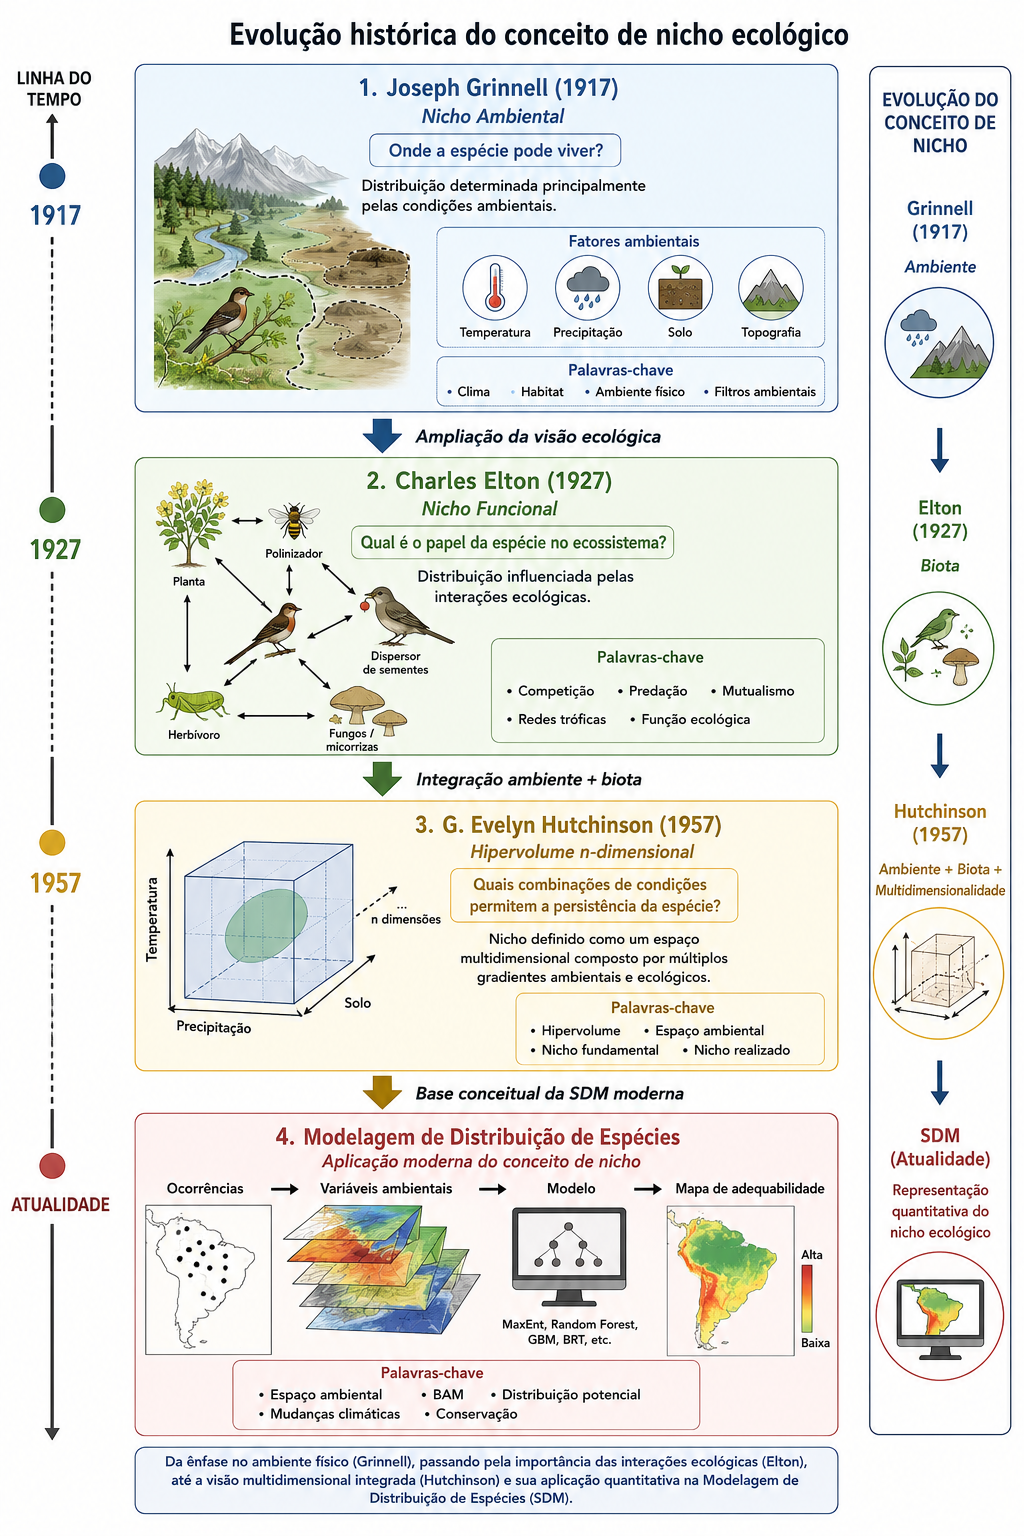
\includegraphics[width=0.9\textwidth]{figuras/unidade01/evolucao_conceito_nicho.png}
	\caption{
		Evolução histórica do conceito de nicho ecológico. A interpretação ambiental de Grinnell enfatiza os requisitos físicos necessários à sobrevivência das espécies. A perspectiva funcional de Elton destaca as interações ecológicas e o papel desempenhado pelos organismos nas comunidades. A formulação multidimensional de Hutchinson integra essas abordagens ao definir o nicho como um hipervolume ecológico composto por múltiplos gradientes ambientais e biológicos. Essa síntese constitui a base conceitual da moderna Modelagem de Distribuição de Espécies.
	}
	\label{fig:evolucao_nicho}
\end{figure}

A Figura~\ref{fig:evolucao_nicho} resume a trajetória histórica do conceito de nicho ecológico. Observa-se que a evolução conceitual não representa uma substituição entre teorias, mas um processo de ampliação progressiva da compreensão sobre os mecanismos que estruturam a distribuição das espécies.

De forma geral, a evolução histórica do conceito pode ser entendida em três grandes etapas:

\begin{enumerate}
	
	\item Uma fase inicialmente centrada nas condições ambientais necessárias à sobrevivência das espécies;
	
	\item Uma fase que incorporou explicitamente as interações ecológicas e o papel funcional dos organismos nas comunidades;
	
	\item Uma fase integradora que formalizou matematicamente o nicho como um espaço multidimensional composto por múltiplos fatores ambientais e ecológicos.
	
\end{enumerate}

Essa progressão reflete o próprio desenvolvimento da Ecologia como ciência. À medida que novos conhecimentos foram acumulados, tornou-se evidente que nenhum fator isolado seria capaz de explicar completamente os padrões observados de distribuição geográfica.

A partir desse contexto histórico emergiram três interpretações clássicas que continuam exercendo forte influência sobre a Ecologia contemporânea e sobre a Modelagem de Distribuição de Espécies.

\begin{table}[H]
	\centering
	\caption{Síntese das principais interpretações históricas do nicho ecológico e sua relação com a Modelagem de Distribuição de Espécies.}
	\label{tab:conceitos_nicho}
	
	\begin{tabular}{p{3cm}p{2.5cm}p{4cm}p{5cm}}
		\toprule
		
		\textbf{Conceito} &
		\textbf{Autor} &
		\textbf{Definição central} &
		\textbf{Relação com SDM} \
		
		\midrule
		
		Nicho de Grinnell &
		Grinnell (1917) &
		Conjunto de condições ambientais necessárias para a sobrevivência da espécie &
		Base da utilização de variáveis climáticas, topográficas e edáficas \
		
		Nicho de Elton &
		Elton (1927) &
		Papel funcional da espécie na comunidade ecológica &
		Fundamenta a incorporação de interações ecológicas em modelos de distribuição \
		
		Nicho de Hutchinson &
		Hutchinson (1957) &
		Hipervolume multidimensional definido por variáveis ambientais e ecológicas &
		Base teórica moderna da Modelagem de Distribuição de Espécies \
		
		Nicho Fundamental &
		Hutchinson (1957) &
		Conjunto potencial de condições compatíveis com a persistência da espécie &
		Representa o limite teórico da distribuição potencial \
		
		Nicho Realizado &
		Hutchinson (1957) &
		Porção efetivamente ocupada sob restrições ecológicas e históricas &
		Representa a fração normalmente amostrada por dados de ocorrência \
		
		\bottomrule
	\end{tabular}
	
\end{table}

A Tabela~\ref{tab:conceitos_nicho} sintetiza as principais contribuições históricas para o desenvolvimento do conceito de nicho ecológico. Embora simplificada, essa síntese evidencia como diferentes interpretações contribuíram para a construção da estrutura conceitual utilizada atualmente em estudos de distribuição de espécies.

É importante destacar que a moderna Modelagem de Distribuição de Espécies não adota exclusivamente nenhuma dessas definições. Na prática, os modelos contemporâneos combinam elementos das diferentes perspectivas, dependendo da pergunta ecológica, dos dados disponíveis e da escala espacial analisada.

Por exemplo, projeções climáticas globais frequentemente utilizam predominantemente a perspectiva grinnelliana, enquanto estudos que incorporam competição, mutualismos ou interações tróficas aproximam-se mais da visão eltoniana. Já a representação matemática do nicho em múltiplas dimensões ambientais deriva diretamente da formulação de Hutchinson e constitui a base conceitual da maioria dos algoritmos utilizados atualmente.

Nos tópicos seguintes serão discutidas em maior profundidade as contribuições individuais de Grinnell, Elton e Hutchinson, destacando suas implicações para a compreensão da distribuição geográfica das espécies e para a construção de modelos ecológicos preditivos.

%================================================
\subsection{O nicho de Grinnell}
%================================================

A primeira formulação moderna do conceito de nicho ecológico é geralmente atribuída ao naturalista e zoólogo norte-americano Joseph Grinnell, que publicou suas ideias em uma série de trabalhos desenvolvidos entre 1914 e 1928, com destaque para o artigo clássico de 1917 intitulado \textit{The Niche-Relationships of the California Thrasher} \parencite{grinnell1917}.

Embora o termo nicho já tivesse sido utilizado anteriormente por outros autores, foi Grinnell quem estabeleceu uma definição ecológica mais consistente e operacional do conceito. Sua principal preocupação era compreender por que determinadas espécies apresentavam distribuições geográficas específicas e quais fatores ambientais limitavam sua ocorrência.

Para Grinnell, cada espécie ocupa uma posição particular na natureza determinada principalmente pelas condições físicas e ambientais necessárias para sua sobrevivência. Em sua interpretação, o nicho ecológico representa o conjunto de características ambientais que permite a persistência de uma espécie em determinado local.

Essa visão surgiu em um período histórico marcado pelo desenvolvimento da Biogeografia e pelo crescente interesse em compreender os padrões espaciais da biodiversidade observados em diferentes regiões do planeta. As grandes expedições científicas do século XIX haviam revelado que espécies semelhantes frequentemente ocupavam ambientes distintos e que muitas distribuições apresentavam limites geográficos relativamente bem definidos.

A principal questão enfrentada pelos ecólogos da época era compreender por que esses limites existiam.

A interpretação proposta por Grinnell sugeria que os organismos eram restringidos por fatores ambientais que definiam as condições necessárias para sua sobrevivência. Dessa forma, a distribuição geográfica observada seria consequência direta das exigências ambientais da espécie e da disponibilidade dessas condições na paisagem.

Sob essa perspectiva, fatores como temperatura, precipitação, umidade, altitude, disponibilidade hídrica e características físicas do ambiente tornam-se os principais determinantes da distribuição das espécies.

Em termos modernos, a abordagem grinnelliana pode ser entendida como uma interpretação predominantemente ambiental do nicho ecológico.

\begin{conceito}
	Na perspectiva de Grinnell, o nicho ecológico corresponde ao conjunto de condições ambientais necessárias para que uma espécie sobreviva, cresça e mantenha populações viáveis em determinada região.
\end{conceito}

Essa interpretação exerceu enorme influência sobre o desenvolvimento posterior da Ecologia, especialmente sobre áreas como Biogeografia, Macroecologia e Modelagem de Distribuição de Espécies.

De fato, a maioria dos modelos de distribuição utilizados atualmente possui forte herança grinnelliana. Quando um pesquisador utiliza variáveis climáticas para explicar a ocorrência de uma espécie, está implicitamente assumindo que a distribuição geográfica observada reflete, ao menos parcialmente, as condições ambientais toleradas pela espécie.

Por essa razão, variáveis derivadas de bases climáticas globais, como WorldClim e CHELSA, são amplamente utilizadas em estudos de SDM. Temperatura média anual, precipitação anual, sazonalidade climática, temperatura mínima do mês mais frio, precipitação do trimestre mais seco e diversas outras variáveis bioclimáticas representam aproximações dos filtros ambientais que estruturam a distribuição das espécies.

Essa relação entre ambiente e distribuição pode ser observada em praticamente todos os biomas do planeta.

Florestas tropicais úmidas predominam em regiões quentes e com elevada disponibilidade hídrica. Savanas desenvolvem-se em áreas sujeitas a maior sazonalidade climática. Tundras ocorrem sob baixas temperaturas e curtas estações de crescimento. Desertos ocupam regiões onde a limitação hídrica impõe fortes restrições fisiológicas aos organismos.

Esses padrões sugerem que o clima atua como um dos principais filtros ambientais em escalas continentais e globais.

\begin{atencao}
	Embora fatores climáticos sejam frequentemente dominantes em escalas amplas, sua importância relativa tende a diminuir em escalas locais, onde processos relacionados ao solo, à topografia, à hidrologia e às interações ecológicas tornam-se progressivamente mais importantes.
\end{atencao}

A importância dos filtros ambientais pode ser compreendida a partir da fisiologia dos organismos. Toda espécie apresenta limites de tolerância para variáveis ambientais específicas. Temperaturas excessivamente elevadas ou reduzidas podem comprometer processos metabólicos fundamentais. Deficiências hídricas prolongadas podem limitar crescimento e reprodução. Alterações na sazonalidade climática podem modificar padrões fenológicos, taxas de recrutamento e dinâmica populacional.

Consequentemente, a distribuição geográfica das espécies tende a refletir a distribuição espacial das condições ambientais compatíveis com seus limites fisiológicos.

Essa ideia constitui uma das bases da moderna teoria dos filtros ambientais (\textit{environmental filtering}), segundo a qual a composição das comunidades ecológicas é fortemente influenciada pelas características ambientais disponíveis \parencite{keddy1992,weiher1998,cornwell2006}.

Segundo essa perspectiva, apenas espécies cujos atributos funcionais sejam compatíveis com as condições locais conseguem persistir em determinado ambiente. Assim, o clima atua como um filtro inicial que restringe quais organismos podem ocupar determinada região.

Essa lógica é particularmente relevante em estudos de mudanças climáticas globais.

À medida que temperatura, precipitação e sazonalidade se alteram ao longo do tempo, os filtros ambientais também se modificam. Como consequência, áreas atualmente adequadas podem tornar-se inadequadas, enquanto novas regiões podem passar a apresentar condições favoráveis para determinadas espécies.

Grande parte das projeções climáticas realizadas em Modelagem de Distribuição de Espécies baseia-se precisamente nessa interpretação. Os modelos assumem que a distribuição atual da espécie fornece informações sobre suas preferências ambientais e utilizam essas relações para estimar possíveis deslocamentos futuros das áreas climaticamente adequadas.

No contexto amazônico, essa abordagem possui relevância especial.

A Amazônia abriga uma das maiores diversidades arbóreas do planeta e apresenta forte heterogeneidade climática, edáfica e hidrológica. Mesmo dentro de uma mesma floresta tropical úmida, gradientes de precipitação, duração da estação seca, disponibilidade hídrica e fertilidade do solo podem influenciar significativamente a composição florística e a distribuição das espécies arbóreas.

Diversos estudos demonstram que a distribuição de espécies amazônicas está associada a gradientes ambientais relacionados à precipitação anual, sazonalidade climática, disponibilidade hídrica e características edáficas \parencite{tersteege2006,tuomisto2019,esquivel2020}.

Essa relação é particularmente importante para espécies de grande porte, como \textit{Dinizia excelsa}, que frequentemente apresentam exigências ambientais específicas relacionadas à estabilidade climática, disponibilidade hídrica e condições adequadas para crescimento ao longo de décadas ou séculos.

A Figura~\ref{fig:unidade01_variaveis_patchwork} ilustra precisamente essa lógica. Os registros de ocorrência de \textit{Dinizia excelsa} encontram-se distribuídos sobre gradientes ambientais representados por temperatura média anual, sazonalidade térmica, precipitação anual e sazonalidade da precipitação. Essas variáveis representam componentes centrais da interpretação grinnelliana do nicho ecológico, pois descrevem condições ambientais capazes de influenciar diretamente o desempenho fisiológico da espécie.

\begin{figure}[H]
	\centering
	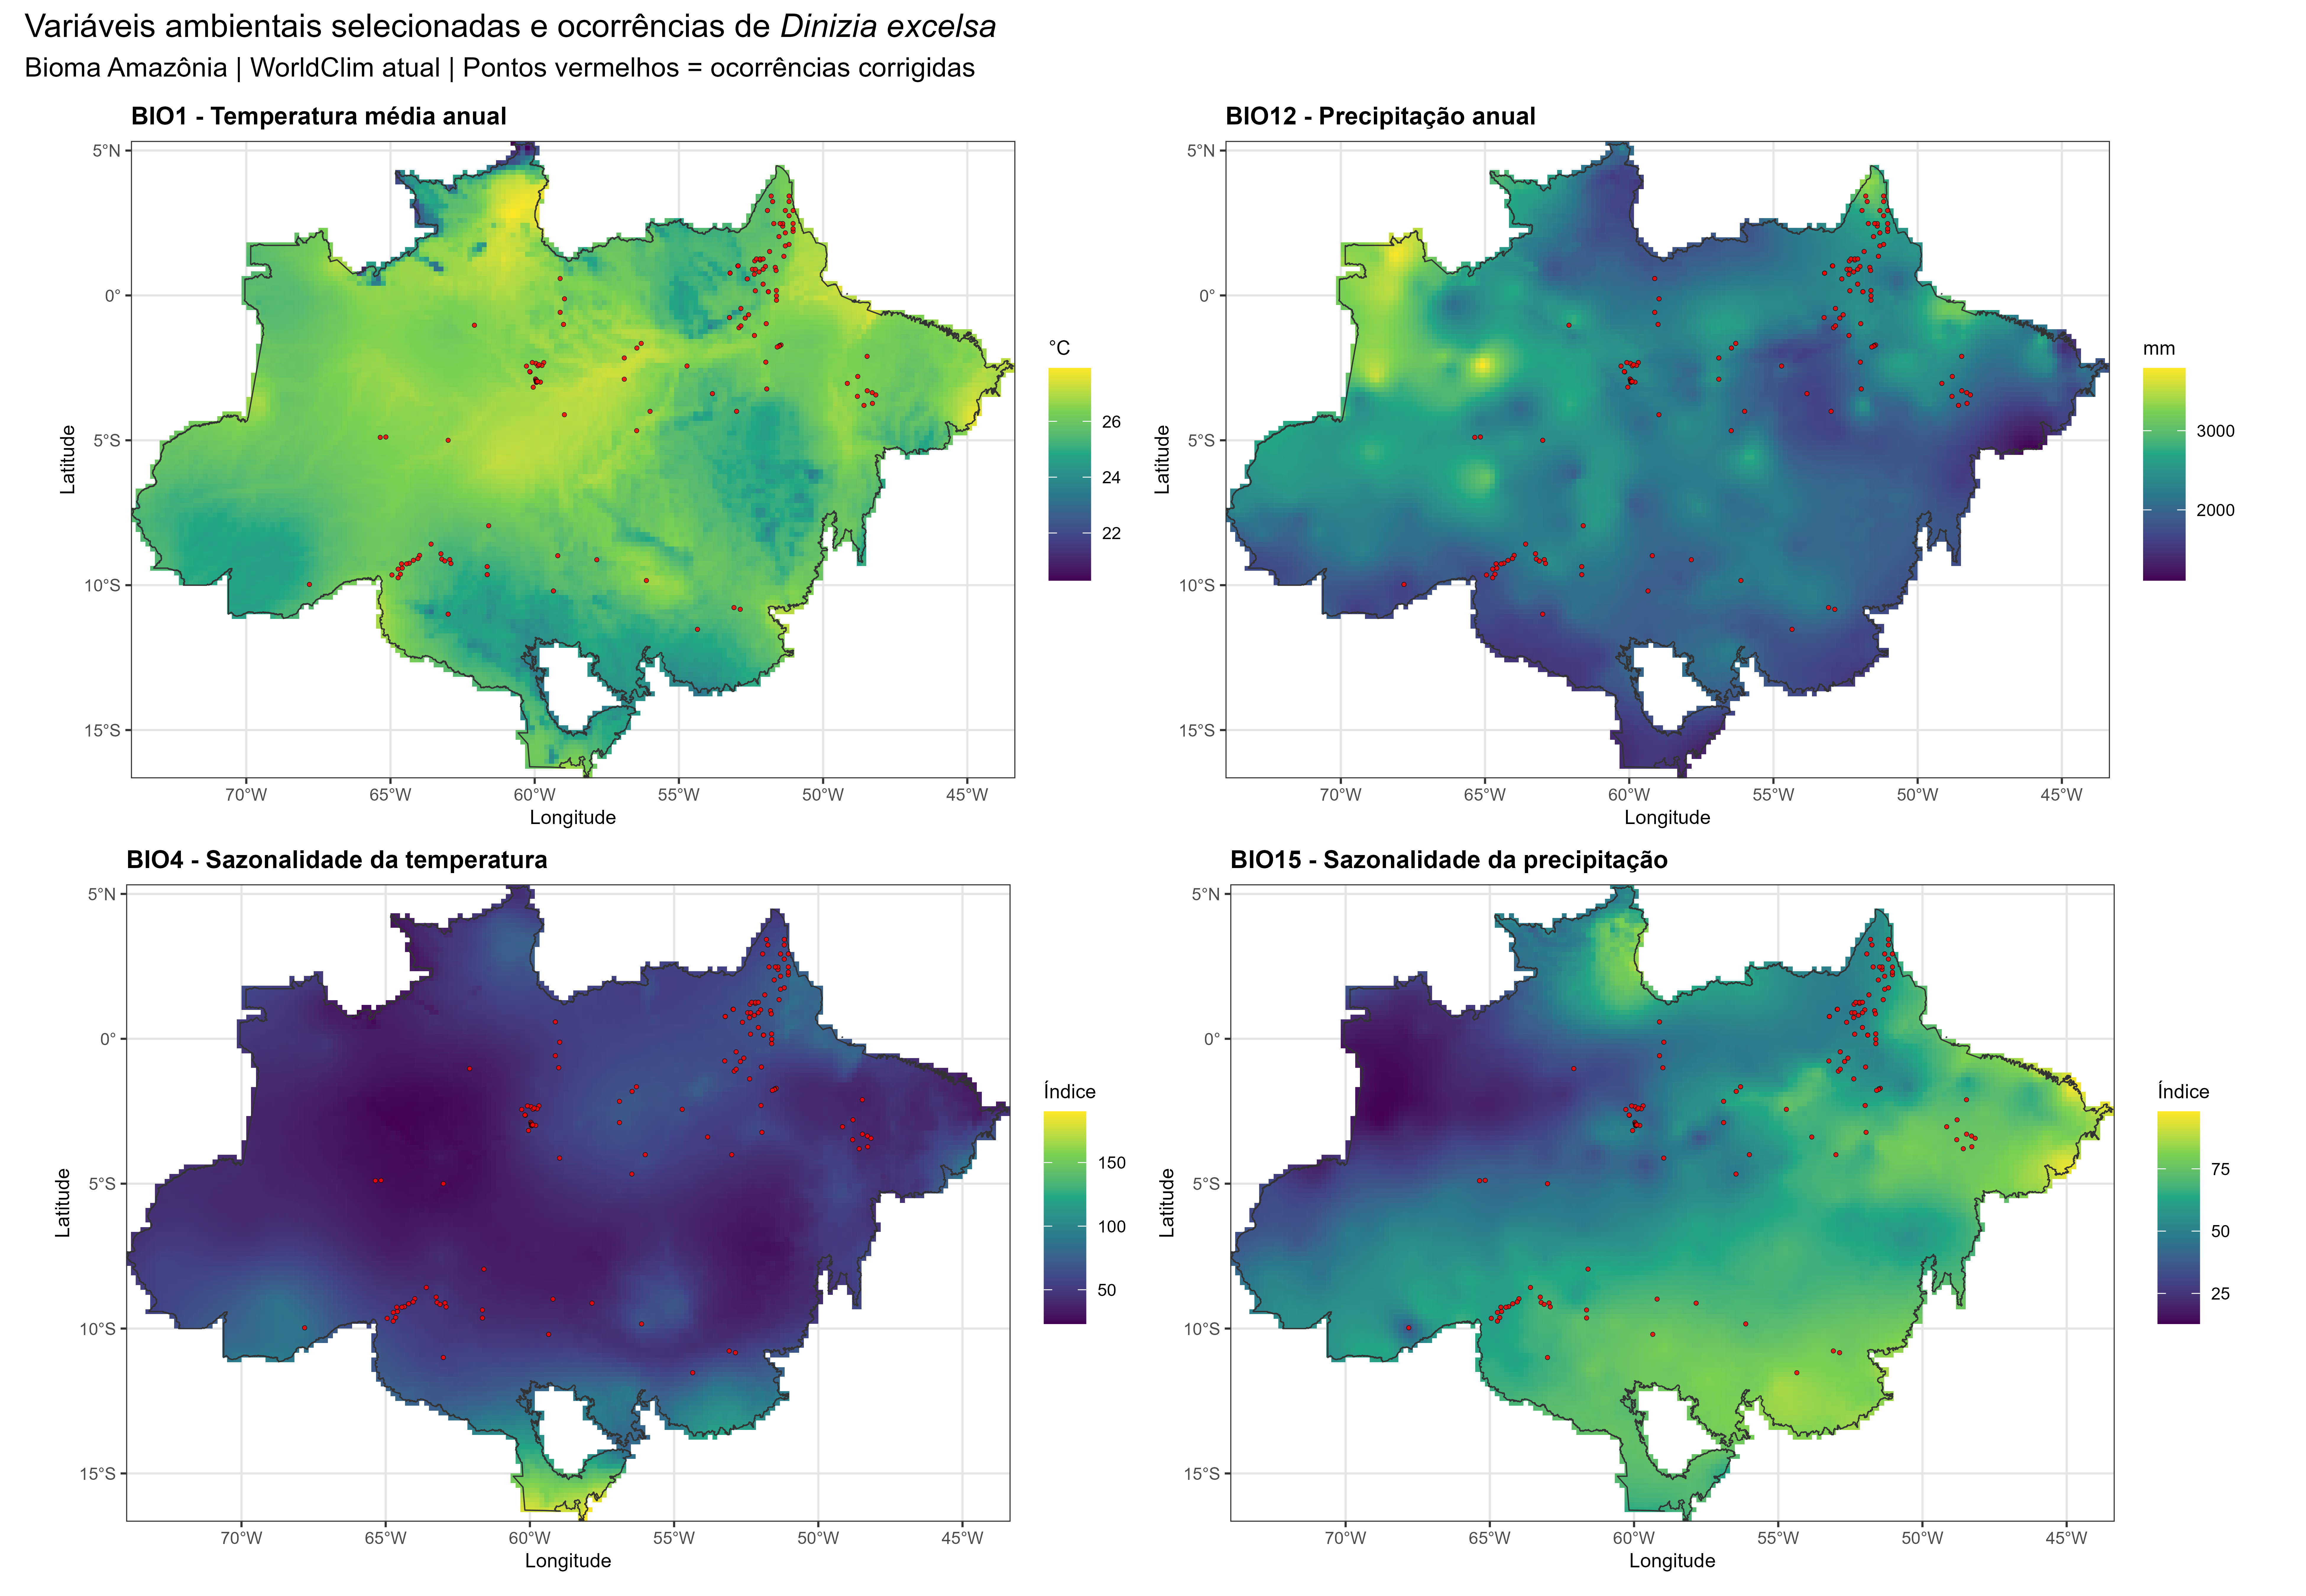
\includegraphics[width=\textwidth]
	{figuras/unidade01/unidade01_mapas_variaveis_patchwork_dinizia.png}
	\caption{
		Gradientes ambientais associados às ocorrências de \textit{Dinizia excelsa} no bioma Amazônia. As variáveis representadas incluem temperatura média anual (BIO1), sazonalidade da temperatura (BIO4), precipitação anual (BIO12) e sazonalidade da precipitação (BIO15). Na perspectiva grinnelliana, esses gradientes ambientais representam componentes fundamentais do nicho ecológico, atuando como filtros capazes de favorecer ou restringir a ocorrência da espécie.
	}
	\label{fig:unidade01_variaveis_patchwork}
\end{figure}

Observa-se que os registros não estão distribuídos aleatoriamente sobre o espaço geográfico. Pelo contrário, concentram-se em regiões associadas a determinadas combinações ambientais, sugerindo que fatores climáticos desempenham papel importante na definição da distribuição observada da espécie.

Essa observação constitui precisamente o ponto de partida da Modelagem de Distribuição de Espécies. A partir da identificação dessas associações entre ambiente e ocorrência, os modelos procuram estimar quais outras regiões apresentam condições semelhantes e, portanto, potencialmente favoráveis à presença da espécie.

Entretanto, apesar de sua enorme importância, a interpretação grinnelliana apresenta limitações importantes.

Nem toda região climaticamente adequada encontra-se necessariamente ocupada por uma espécie. Barreiras geográficas, limitações de dispersão, interações ecológicas negativas, eventos históricos e processos evolutivos também influenciam a distribuição observada. Dessa forma, condições ambientais adequadas representam uma condição necessária, mas frequentemente não suficiente para explicar completamente a ocorrência das espécies.

Essas limitações motivaram o desenvolvimento de interpretações mais amplas do nicho ecológico, incorporando explicitamente as interações entre organismos e seu papel funcional nos ecossistemas.

Foi nesse contexto que surgiu a contribuição de Charles Elton, cuja abordagem ampliou significativamente a compreensão dos processos responsáveis pela distribuição e coexistência das espécies nas comunidades ecológicas.

%================================================
\subsection{O nicho de Elton}
%================================================

Embora a interpretação proposta por Joseph Grinnell tenha representado um avanço fundamental para a compreensão da distribuição geográfica das espécies, ela concentrava-se predominantemente nos componentes físicos do ambiente. Entretanto, à medida que a Ecologia avançava como disciplina científica, tornou-se cada vez mais evidente que a simples presença de condições ambientais adequadas não era suficiente para explicar completamente os padrões observados na natureza.

Diversas espécies apresentavam distribuições que não podiam ser compreendidas apenas por fatores climáticos ou fisiológicos. Em muitos casos, organismos estavam ausentes de áreas aparentemente adequadas ou apresentavam abundâncias extremamente distintas em ambientes com características físicas semelhantes. Essas observações sugeriam que outros processos ecológicos desempenhavam papel importante na determinação da ocorrência das espécies.

Foi nesse contexto que o ecólogo britânico Charles Sutherland Elton publicou, em 1927, a obra clássica \textit{Animal Ecology}, considerada um marco na consolidação da Ecologia moderna \parencite{elton1927}. Diferentemente da abordagem de Grinnell, Elton direcionou sua atenção para as relações ecológicas estabelecidas entre os organismos e para o papel funcional que cada espécie desempenha dentro de uma comunidade biológica.

Na perspectiva eltoniana, o nicho ecológico não é definido apenas pelas condições ambientais necessárias para a sobrevivência da espécie, mas também pela forma como ela utiliza recursos, interage com outros organismos e participa dos fluxos de energia e matéria nos ecossistemas \parencite{elton1927,soberon2007}.

Assim, enquanto a visão grinnelliana pode ser resumida pela pergunta:

\begin{quote}
	\textit{Onde a espécie pode viver?}
\end{quote}

a perspectiva de Elton procura responder uma questão diferente:

\begin{quote}
	\textit{Qual é o papel da espécie no ecossistema?}
\end{quote}

Essa mudança de enfoque representou uma transformação profunda na compreensão do nicho ecológico. O organismo deixou de ser visto apenas como um receptor passivo das condições ambientais e passou a ser interpretado como um agente ativo que estabelece relações ecológicas complexas com outros componentes da comunidade.

\begin{conceito}
	Na interpretação de Elton, o nicho ecológico corresponde ao papel funcional desempenhado por uma espécie dentro do ecossistema, incluindo suas relações tróficas, seus recursos utilizados, seus inimigos naturais, seus competidores e suas interações ecológicas.
\end{conceito}

Uma das principais contribuições de Elton foi enfatizar a importância das redes tróficas para compreender a organização das comunidades biológicas. Segundo essa perspectiva, cada espécie ocupa uma posição específica dentro da estrutura alimentar do ecossistema, influenciando e sendo influenciada por outros organismos \parencite{elton1927,pimm1982}.

Em comunidades vegetais, por exemplo, as plantas não interagem apenas com o ambiente físico. Elas estabelecem relações complexas com polinizadores, dispersores de sementes, herbívoros, patógenos, fungos micorrízicos e espécies competidoras. Essas interações podem aumentar, reduzir ou até mesmo impedir a ocorrência de determinadas espécies em locais que, sob uma perspectiva puramente climática, seriam considerados adequados.

Da mesma forma, em comunidades animais, a distribuição de uma espécie frequentemente depende da disponibilidade de recursos alimentares, da presença de presas, da ocorrência de predadores e da intensidade da competição interespecífica. Em muitos casos, esses fatores podem ser mais importantes do que as próprias condições climáticas na determinação dos padrões de ocorrência observados em escala local \parencite{begon2006,ricklefs2010}.

A competição constitui um dos exemplos clássicos da influência das interações ecológicas sobre a distribuição das espécies. Segundo o princípio da exclusão competitiva, duas espécies que utilizam exatamente os mesmos recursos dificilmente conseguem coexistir indefinidamente no mesmo ambiente \parencite{gause1934}. Como consequência, a presença de uma espécie pode restringir a distribuição de outra mesmo quando ambas apresentam exigências ambientais semelhantes.

De maneira semelhante, interações positivas também podem influenciar fortemente a distribuição geográfica dos organismos. Relações mutualísticas, como aquelas observadas entre plantas e polinizadores ou entre raízes e fungos micorrízicos, frequentemente ampliam a capacidade das espécies de persistirem em determinados ambientes \parencite{bronstein1994}. Em alguns casos, a ausência de parceiros mutualistas pode limitar a expansão geográfica de uma espécie, mesmo em regiões climaticamente adequadas.

Esses exemplos demonstram que a distribuição observada dos organismos não resulta apenas da disponibilidade de condições ambientais favoráveis. Ela também reflete a complexa rede de interações ecológicas estabelecidas entre os organismos ao longo do tempo.

A importância das interações ecológicas torna-se particularmente evidente quando analisamos comunidades altamente diversas, como as florestas tropicais. A Amazônia abriga milhares de espécies vegetais que coexistem em uma mesma paisagem, compartilhando recursos e interagindo continuamente em diferentes níveis ecológicos. Processos relacionados à competição por luz, água e nutrientes, bem como interações com dispersores, polinizadores e inimigos naturais, contribuem para a organização espacial dessas comunidades \parencite{terborgh2012,levin2013}.

Nesse contexto, duas regiões com condições climáticas semelhantes podem apresentar composições florísticas distintas em função das diferenças nas interações ecológicas locais. Essa observação evidencia uma limitação importante da interpretação exclusivamente grinnelliana da distribuição das espécies.

Para a Modelagem de Distribuição de Espécies, a perspectiva eltoniana possui implicações profundas. Grande parte dos modelos atualmente utilizados é construída a partir de variáveis ambientais, especialmente climáticas, topográficas e edáficas. Essas variáveis representam adequadamente muitos dos filtros ambientais discutidos na seção anterior, mas frequentemente não capturam explicitamente as interações ecológicas que influenciam a ocorrência das espécies \parencite{guisan2005predicting,elith2009}.

Como consequência, a maioria dos modelos correlativos tradicionais descreve predominantemente o chamado nicho grinnelliano, enquanto os componentes eltonianos permanecem parcial ou totalmente ausentes da análise \parencite{soberon2007}. Isso não significa que as interações ecológicas sejam irrelevantes, mas apenas que elas raramente estão disponíveis em bases de dados espaciais com abrangência e resolução comparáveis às variáveis climáticas.

Essa limitação constitui uma das principais fronteiras atuais da Modelagem de Distribuição de Espécies. Nas últimas décadas, diversos estudos têm buscado incorporar explicitamente variáveis relacionadas à estrutura das comunidades, abundância de espécies associadas, redes de interação e características funcionais dos organismos \parencite{wisz2013,kissling2012}. Essas abordagens procuram aproximar os modelos da complexidade ecológica observada nos ecossistemas naturais.

Entretanto, mesmo com os avanços recentes, a representação completa das interações ecológicas continua sendo um dos maiores desafios da modelagem preditiva. Muitas relações biológicas são dinâmicas, contextuais e dependentes da escala espacial considerada. Além disso, a disponibilidade de dados ecológicos detalhados ainda é significativamente menor que a disponibilidade de informações climáticas globais.

\begin{atencao}
	A ausência de variáveis bióticas em um modelo de distribuição não implica que as interações ecológicas sejam irrelevantes. Significa apenas que essas informações frequentemente não estão disponíveis em escala espacial compatível com a modelagem realizada.
\end{atencao}

Em estudos envolvendo árvores amazônicas de grande porte, por exemplo, a ocorrência de uma espécie pode depender não apenas das condições climáticas adequadas, mas também da presença de dispersores eficientes, de padrões específicos de recrutamento, da dinâmica sucessional da floresta e da intensidade da competição por recursos. Ignorar completamente esses fatores pode limitar a capacidade de interpretação ecológica dos modelos produzidos.

No caso de \textit{Dinizia excelsa}, espécie utilizada como estudo de caso ao longo deste livro, a distribuição observada provavelmente reflete não apenas gradientes climáticos e ambientais, mas também processos relacionados à dispersão de sementes, dinâmica populacional, história de ocupação da paisagem e interações ecológicas acumuladas ao longo de séculos de desenvolvimento florestal.

Apesar dessas limitações, a contribuição de Elton foi fundamental para ampliar a compreensão dos fatores responsáveis pela distribuição das espécies. Sua abordagem demonstrou que a distribuição geográfica não pode ser explicada exclusivamente por condições ambientais, exigindo a consideração das interações ecológicas que estruturam as comunidades naturais.

Entretanto, tanto a perspectiva de Grinnell quanto a de Elton ainda careciam de uma estrutura formal capaz de integrar simultaneamente múltiplos fatores ambientais e ecológicos. Essa integração seria realizada algumas décadas mais tarde por George Evelyn Hutchinson, cuja formulação do nicho como um hipervolume multidimensional transformaria profundamente a Ecologia moderna e estabeleceria as bases conceituais da atual Modelagem de Distribuição de Espécies.

%================================================
\subsection{O nicho de Hutchinson}
%================================================

As contribuições de Grinnell e Elton estabeleceram dois pilares fundamentais para a compreensão da distribuição das espécies. Enquanto Grinnell enfatizou a importância das condições ambientais necessárias para a sobrevivência dos organismos, Elton destacou o papel das interações ecológicas e da função desempenhada pelas espécies dentro das comunidades biológicas.

Entretanto, apesar de seu enorme valor conceitual, ambas as interpretações apresentavam uma limitação importante: nenhuma delas fornecia uma estrutura quantitativa capaz de integrar simultaneamente os múltiplos fatores ambientais e ecológicos que influenciam a ocorrência das espécies.

Foi nesse contexto que o ecólogo britânico George Evelyn Hutchinson publicou, em 1957, o trabalho considerado um dos mais influentes da história da Ecologia moderna: \textit{Concluding Remarks}, resultado de um simpósio realizado no Cold Spring Harbor Laboratory \parencite{hutchinson1957}. Nesse artigo, Hutchinson propôs uma formulação matemática e ecológica do nicho que transformaria profundamente a forma como ecólogos compreendem a distribuição dos organismos.

A principal inovação de Hutchinson foi definir o nicho ecológico como um \textbf{hipervolume multidimensional}, no qual cada dimensão representa uma variável ambiental ou ecológica relevante para a sobrevivência, crescimento e reprodução de uma espécie.

Essa definição marcou uma mudança conceitual profunda. O nicho deixou de ser interpretado apenas como um conjunto de condições ambientais ou como um papel funcional na comunidade e passou a ser entendido como uma região específica de um espaço abstrato composto por múltiplos gradientes ecológicos.

Segundo Hutchinson, uma espécie pode persistir apenas dentro de determinados limites para cada variável ambiental relevante. Quando essas condições são atendidas simultaneamente, a espécie apresenta crescimento populacional positivo e consegue manter populações viáveis ao longo do tempo. Fora desses limites, a persistência populacional torna-se inviável.

\begin{conceito}
	Hutchinson definiu o nicho ecológico como um hipervolume n-dimensional, no qual cada dimensão representa uma variável ambiental ou ecológica relevante para a persistência da espécie. O nicho corresponde ao conjunto de combinações de condições sob as quais a população apresenta crescimento positivo.
\end{conceito}

A importância dessa definição torna-se mais evidente quando consideramos que os organismos raramente respondem a apenas uma variável ambiental. Na natureza, espécies estão simultaneamente sujeitas a múltiplos fatores, como temperatura, precipitação, disponibilidade hídrica, fertilidade do solo, luminosidade, sazonalidade climática, competição, predação e disponibilidade de recursos.

Cada um desses fatores pode ser representado como um eixo dentro do hipervolume ecológico proposto por Hutchinson.

Para ilustrar esse conceito, imagine inicialmente uma espécie cuja ocorrência dependa apenas da temperatura. Nesse caso, o nicho poderia ser representado por um simples intervalo ao longo de uma única dimensão. Se adicionarmos a precipitação como segundo fator limitante, o nicho passa a ocupar uma área bidimensional. Com a inclusão de novas variáveis ambientais, surgem volumes tridimensionais, tetradimensionais e, eventualmente, espaços com dezenas de dimensões.

Embora esses espaços multidimensionais não possam ser visualizados diretamente, eles representam de forma muito mais realista a complexidade ecológica enfrentada pelos organismos na natureza.

\begin{figure}[H]
	\centering
	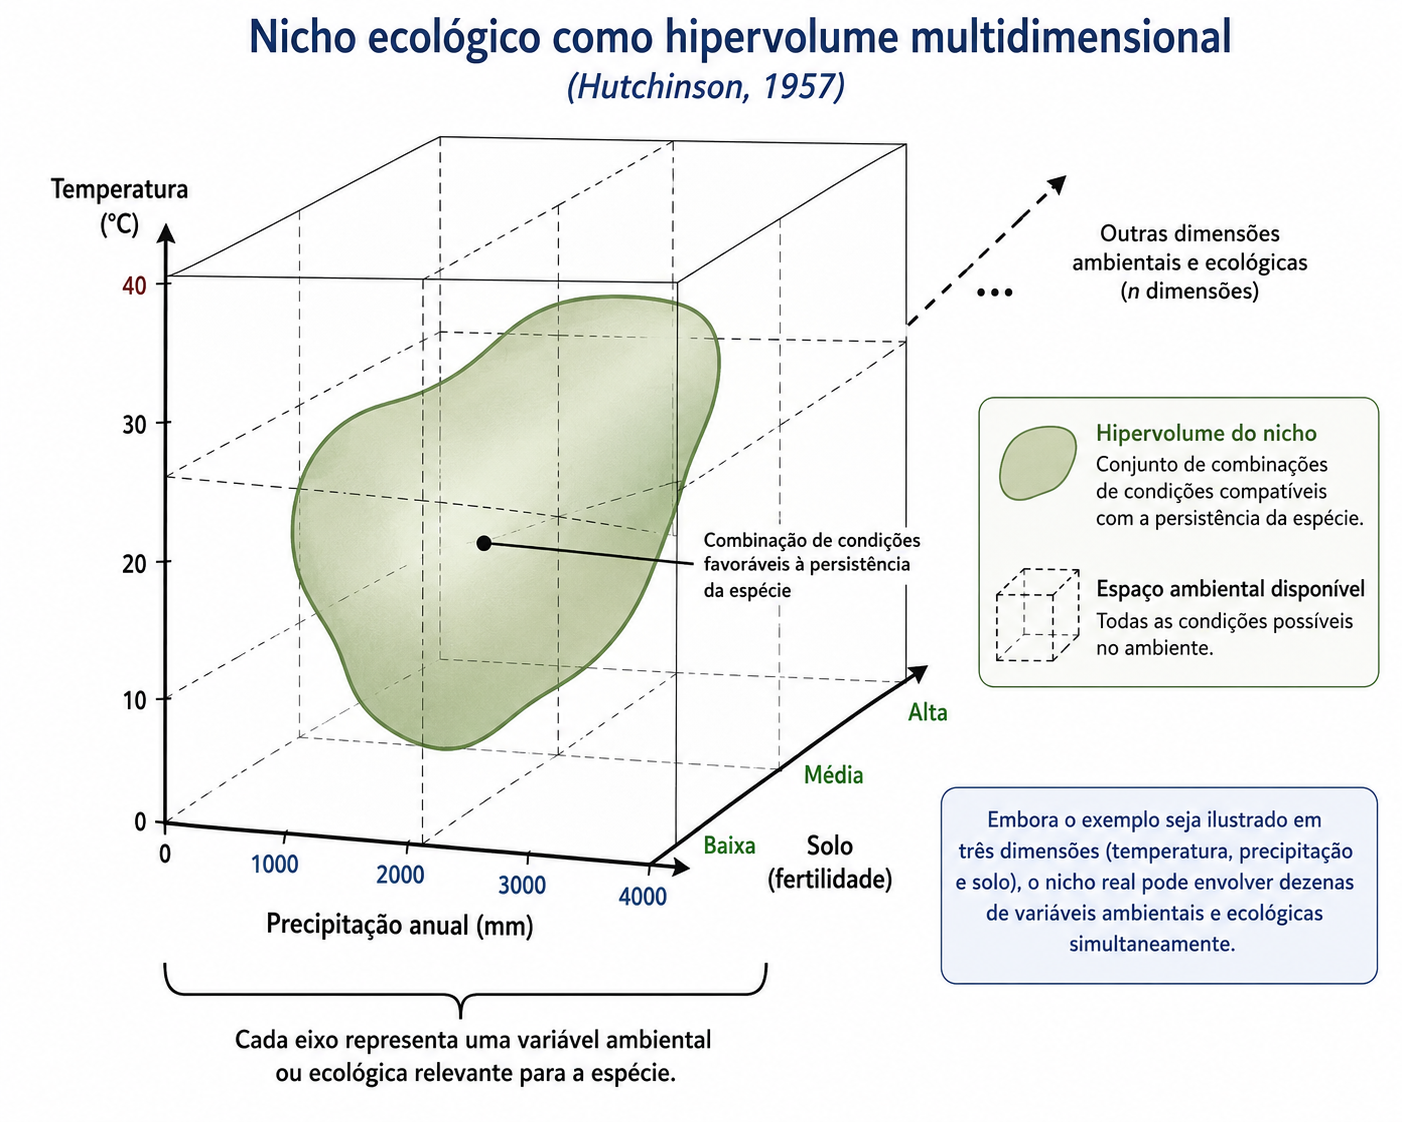
\includegraphics[width=0.85\textwidth]{figuras/unidade01/hipervolume_hutchinson.png}
	\caption{
		Representação conceitual do nicho ecológico como hipervolume multidimensional segundo Hutchinson. Cada eixo representa uma variável ambiental ou ecológica relevante para a espécie. A região sombreada corresponde ao conjunto de combinações de condições compatíveis com a persistência populacional. Embora ilustrado em poucas dimensões, o nicho real pode envolver dezenas de gradientes ambientais simultâneos.
	}
	\label{fig:hipervolume_hutchinson}
\end{figure}

A Figura~\ref{fig:hipervolume_hutchinson} ilustra a essência da proposta de Hutchinson. Embora a representação gráfica utilize apenas duas ou três dimensões por limitações visuais, o conceito original admite qualquer número de variáveis ecológicas relevantes.

Essa característica torna a formulação de Hutchinson extraordinariamente poderosa para a Ecologia moderna. Diferentemente das abordagens anteriores, ela permite representar simultaneamente fatores climáticos, edáficos, topográficos, fisiológicos e ecológicos dentro de uma única estrutura conceitual.

Além disso, a definição de Hutchinson estabeleceu uma ponte natural entre Ecologia e Matemática, permitindo que conceitos ecológicos fossem formalizados por meio de métodos quantitativos. Essa integração abriu caminho para o desenvolvimento de diversas áreas modernas da Ecologia, incluindo análise multivariada, modelagem ecológica, teoria de nicho, macroecologia e, posteriormente, Modelagem de Distribuição de Espécies.

%================================================
\section{Do espaço geográfico ao espaço ambiental}
%================================================

Um dos conceitos mais importantes para compreender a lógica da Modelagem de Distribuição de Espécies é a distinção entre espaço geográfico e espaço ambiental. Embora esses termos sejam frequentemente utilizados de forma intuitiva, eles representam dimensões conceitualmente distintas da realidade ecológica e constituem a base do raciocínio que sustenta praticamente todos os algoritmos de SDM.

A necessidade de diferenciar esses dois espaços surge diretamente da formulação do nicho ecológico proposta por Hutchinson. Como discutido na seção anterior, o nicho não é definido em termos de coordenadas geográficas, mas sim em função das condições ambientais associadas aos locais onde as espécies vivem. Consequentemente, compreender a distribuição das espécies exige ir além da simples localização geográfica dos organismos e investigar as condições ambientais que caracterizam esses locais \parencite{hutchinson1957,soberon2007}.

Em termos simples, o espaço geográfico corresponde ao mundo físico representado por mapas, coordenadas, pixels, bacias hidrográficas, paisagens, biomas e continentes. É o espaço onde observamos diretamente a ocorrência das espécies e onde são realizadas as amostragens biológicas.

Já o espaço ambiental corresponde ao conjunto de condições ambientais associadas a cada local do espaço geográfico. Temperatura, precipitação, altitude, fertilidade do solo, déficit hídrico, sazonalidade climática, radiação solar e inúmeras outras variáveis constituem dimensões desse espaço ambiental \parencite{franklin2010}.

\begin{conceito}
	O espaço geográfico descreve onde uma espécie ocorre. O espaço ambiental descreve sob quais condições ambientais essa espécie ocorre.
\end{conceito}

Essa distinção pode parecer sutil, mas possui implicações profundas para a interpretação dos modelos de distribuição.

Quando observamos um mapa contendo registros de ocorrência de uma espécie, estamos visualizando padrões no espaço geográfico. Entretanto, os organismos não respondem diretamente às coordenadas geográficas. Uma árvore não reconhece latitude ou longitude; ela responde à disponibilidade de água, temperatura, nutrientes, luz e outras condições ambientais que influenciam seu desempenho fisiológico e ecológico.

Consequentemente, a distribuição geográfica das espécies emerge como uma manifestação espacial de suas respostas ao ambiente.

Essa ideia constitui o fundamento conceitual da Modelagem de Distribuição de Espécies moderna. Em vez de modelar diretamente a posição geográfica dos organismos, os algoritmos procuram identificar relações entre ocorrência e ambiente, inferindo quais combinações de condições ambientais estão associadas à presença da espécie \parencite{guisan2005predicting,elith2009}.

\subsection{Como os modelos conectam esses dois espaços?}

A lógica operacional dos modelos de distribuição pode ser compreendida como uma sequência de etapas que conecta espaço geográfico e espaço ambiental.

Inicialmente, os registros de ocorrência são representados em um mapa geográfico. Cada ocorrência possui uma localização espacial específica, normalmente definida por coordenadas geográficas.

Em seguida, para cada ponto de ocorrência, são extraídas informações ambientais provenientes de camadas climáticas, topográficas, edáficas ou outras variáveis relevantes. Nesse momento, cada registro deixa de ser apenas um ponto no mapa e passa a ser descrito por um conjunto de condições ambientais.

Por exemplo, uma ocorrência de \textit{Dinizia excelsa} pode estar associada aos seguintes valores:

\begin{itemize}
	
	\item Temperatura média anual: 26,5°C;
	
	\item Precipitação anual: 2.350 mm;
	
	\item Sazonalidade da precipitação: 42;
	
	\item Altitude: 115 m.
	
\end{itemize}

Esses valores definem a posição da ocorrência no espaço ambiental.

A partir desse conjunto de informações, os algoritmos procuram identificar padrões e estimar quais combinações ambientais caracterizam os locais ocupados pela espécie. Posteriormente, essas relações são projetadas novamente para toda a paisagem, produzindo mapas de adequabilidade ambiental.

Esse processo pode ser resumido da seguinte forma:

\begin{center}
	
	Ocorrências
	
	$\rightarrow$
	
	Espaço Ambiental
	
	$\rightarrow$
	
	Modelagem
	
	$\rightarrow$
	
	Projeção Espacial
	
	$\rightarrow$
	
	Mapa de Adequabilidade
	
\end{center}

Essa sequência representa a essência de praticamente todos os métodos utilizados em SDM.

\subsection{Visualizando o espaço ambiental}

Uma das maiores dificuldades para iniciantes em Modelagem de Distribuição de Espécies consiste em visualizar o espaço ambiental. Enquanto mapas geográficos são intuitivos, espaços multidimensionais compostos por diversas variáveis ambientais são mais difíceis de representar graficamente.

Uma abordagem comum consiste em utilizar gráficos bivariados ou técnicas de ordenação multivariada, como a Análise de Componentes Principais (PCA), para representar parte da estrutura ambiental dos dados.

A Figura~\ref{fig:unidade01_nicho_tp_dinizia} apresenta um exemplo utilizando temperatura média anual e precipitação anual para representar o espaço climático ocupado por \textit{Dinizia excelsa}.

\begin{figure}[H]
	\centering
	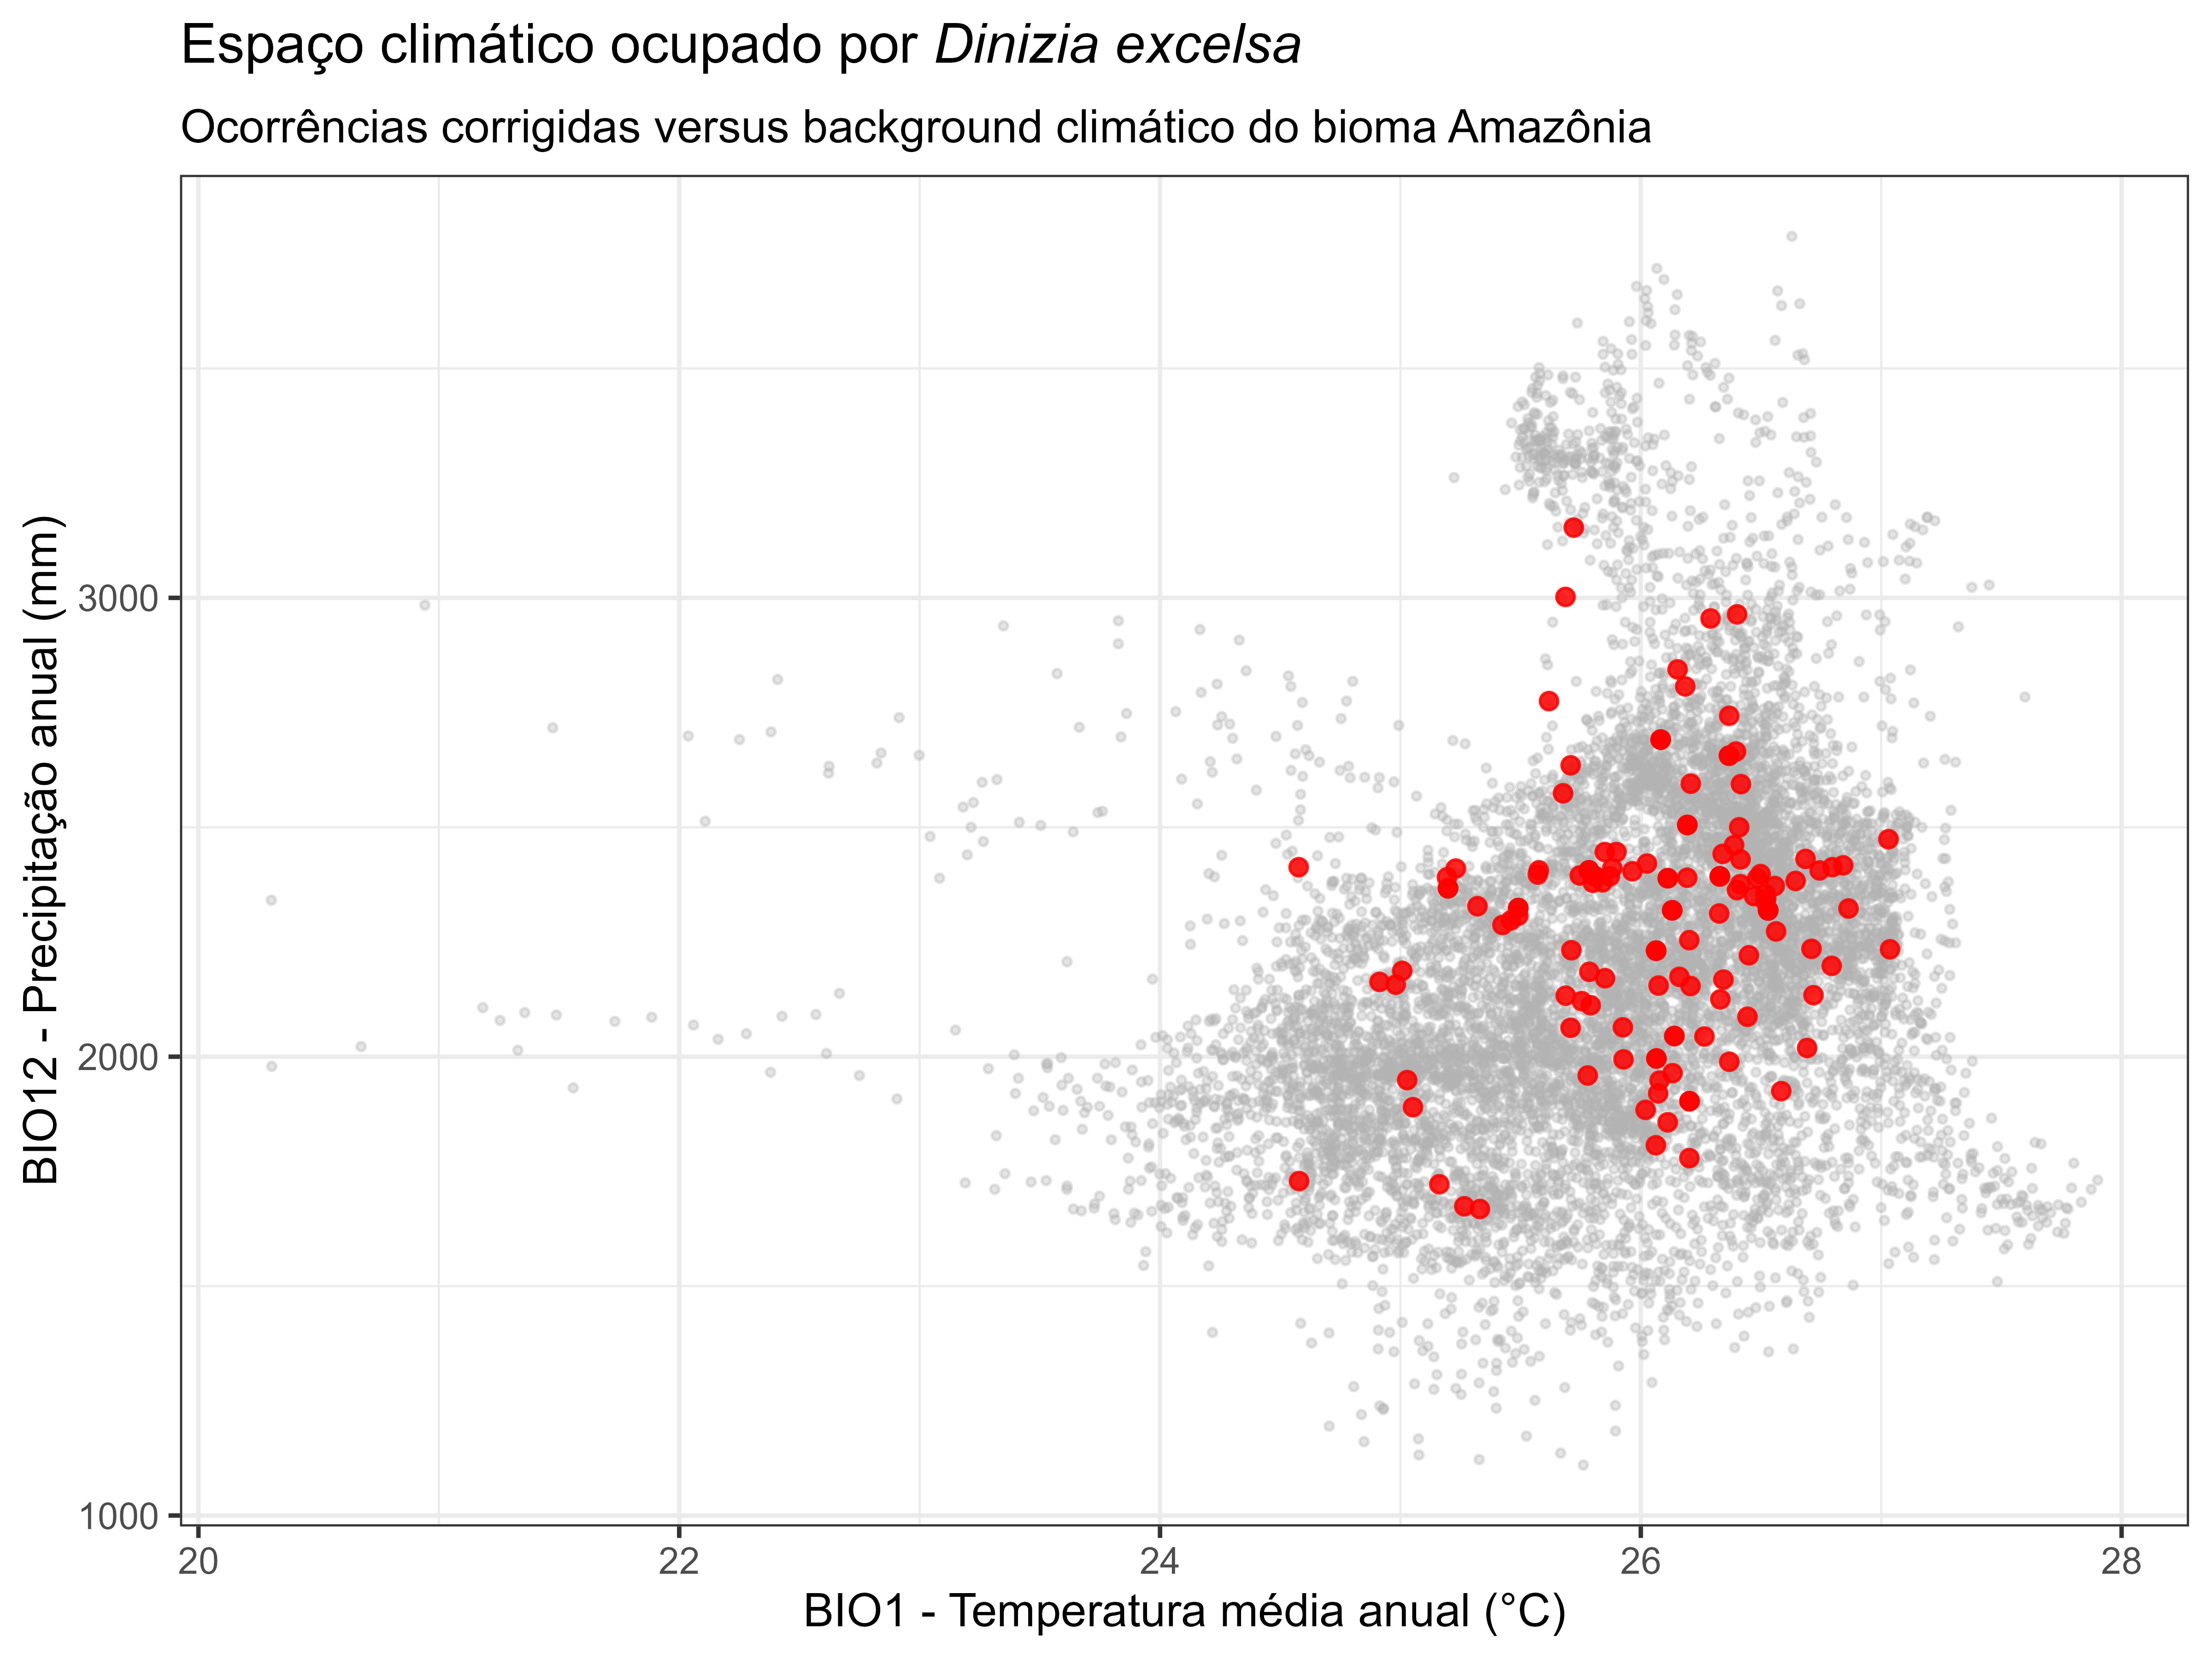
\includegraphics[width=0.85\textwidth]
	{figuras/unidade01/unidade01_nicho_temperatura_precipitacao_dinizia.png}
	\caption{
		Representação do espaço climático ocupado por \textit{Dinizia excelsa} considerando temperatura média anual e precipitação anual. Os pontos cinza representam o ambiente disponível no bioma Amazônia, enquanto os pontos vermelhos representam as condições efetivamente ocupadas pela espécie.
	}
	\label{fig:unidade01_nicho_tp_dinizia}
\end{figure}

Observa-se que os registros de ocorrência ocupam apenas uma fração das condições ambientais disponíveis na Amazônia. Essa região ocupada corresponde a uma projeção simplificada do nicho ecológico da espécie em duas dimensões ambientais.

A interpretação torna-se ainda mais clara quando utilizamos técnicas multivariadas.

\begin{figure}[H]
	\centering
	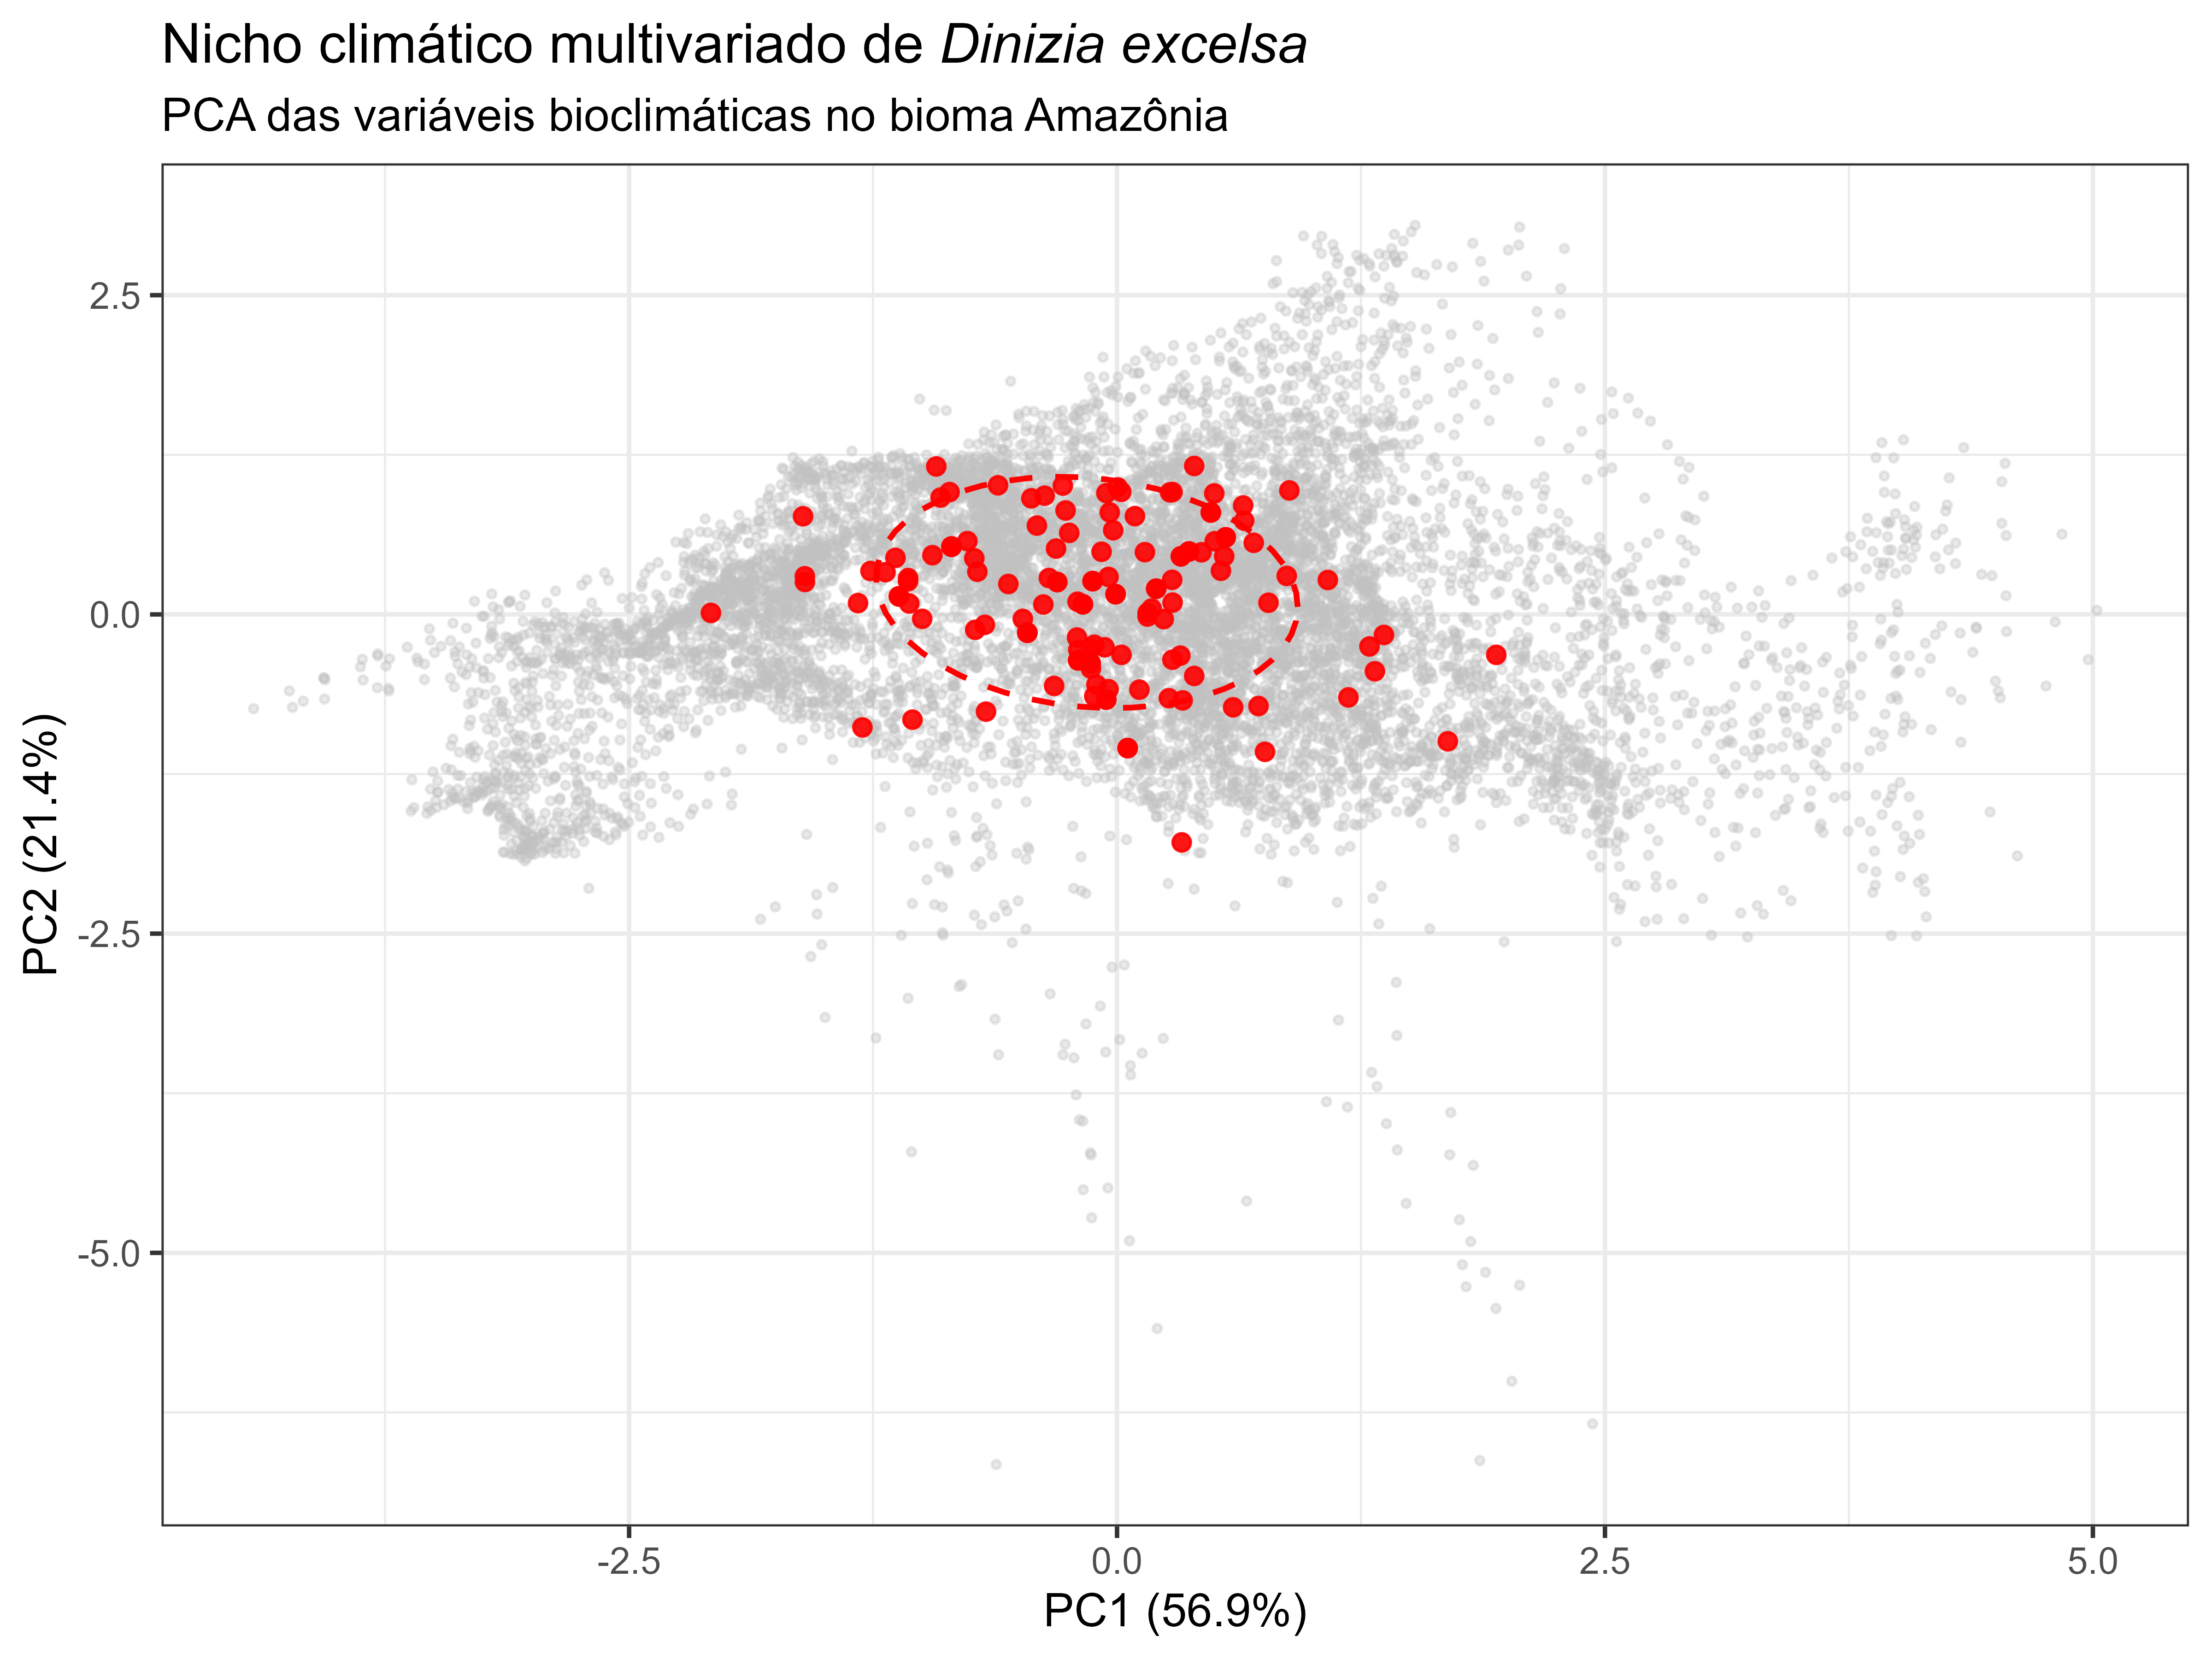
\includegraphics[width=0.85\textwidth]
	{figuras/unidade01/unidade01_pca_nicho_climatico_dinizia.png}
	\caption{
		Representação do espaço ambiental de \textit{Dinizia excelsa} utilizando Análise de Componentes Principais (PCA). Os eixos sintéticos resumem parte da variabilidade climática disponível no bioma Amazônia.
	}
	\label{fig:unidade01_pca_nicho}
\end{figure}

Na Figura~\ref{fig:unidade01_pca_nicho}, as ocorrências são representadas em um espaço ambiental multivariado construído a partir de múltiplas variáveis climáticas. Embora a PCA não represente diretamente o nicho ecológico, ela permite visualizar como a espécie ocupa apenas uma porção do ambiente disponível.

Esse padrão ilustra de forma prática a ideia do hipervolume de Hutchinson discutida anteriormente.

\subsection{Por que essa distinção é tão importante em SDM?}

A distinção entre espaço geográfico e espaço ambiental explica uma característica fundamental dos modelos de distribuição: eles aprendem relações ambientais, não relações geográficas.

Isso significa que dois locais geograficamente distantes podem apresentar elevada adequabilidade ambiental caso possuam condições ambientais semelhantes.

Por outro lado, áreas geograficamente próximas podem apresentar adequabilidade muito diferente caso estejam associadas a condições ambientais distintas.

Essa característica permite que modelos sejam projetados para outras regiões geográficas, para cenários climáticos futuros e até mesmo para períodos paleoclimáticos.

Ao mesmo tempo, ela explica por que a seleção de variáveis ambientais constitui uma das etapas mais importantes de qualquer estudo de SDM. Se as variáveis utilizadas não representarem adequadamente os fatores que influenciam a distribuição da espécie, o modelo poderá identificar padrões estatísticos sem significado ecológico.

Por essa razão, a escolha das variáveis ambientais deve sempre ser orientada por hipóteses ecológicas explícitas e não apenas por disponibilidade de dados ou desempenho estatístico.

A compreensão da relação entre espaço geográfico e espaço ambiental também prepara o leitor para um dos conceitos mais importantes da Modelagem de Distribuição de Espécies moderna: o framework BAM, que integra fatores abióticos, interações bióticas e limitações de dispersão em uma estrutura conceitual unificada para explicar a distribuição das espécies.

%================================================
\section{O framework BAM: ambiente, biota e acessibilidade}
%================================================

Embora o nicho ecológico forneça uma estrutura poderosa para compreender a distribuição das espécies, ecólogos reconheceram ao longo do tempo que a simples existência de condições ambientais adequadas não garante a ocorrência de uma espécie em determinado local.

Muitas regiões apresentam clima, solo e condições ambientais aparentemente favoráveis, mas permanecem desocupadas por determinadas espécies. Em outros casos, espécies persistem em locais que parecem subótimos do ponto de vista ambiental. Essas observações indicam que a distribuição geográfica dos organismos resulta da interação entre múltiplos processos ecológicos e biogeográficos.

Com o objetivo de integrar esses diferentes componentes em uma estrutura conceitual única, Soberón propôs o framework BAM, atualmente considerado uma das bases teóricas mais importantes da Modelagem de Distribuição de Espécies \parencite{soberon2005,soberon2007,soberon2009}.

O acrônimo BAM deriva de três componentes fundamentais:

\begin{itemize}
	
	\item \textbf{B} (\textit{Biotic}) -- fatores bióticos;
	
	\item \textbf{A} (\textit{Abiotic}) -- fatores abióticos;
	
	\item \textbf{M} (\textit{Movement} ou \textit{Mobility}) -- área acessível por dispersão.
	
\end{itemize}

Segundo essa estrutura, a distribuição observada de uma espécie resulta da interação simultânea entre esses três componentes.

\subsection{Componente A: fatores abióticos}

O componente (A) representa o conjunto de condições ambientais compatíveis com a sobrevivência e reprodução da espécie.

Esse componente está intimamente relacionado ao nicho grinnelliano e inclui variáveis como temperatura, precipitação, disponibilidade hídrica, características do solo, topografia e outros fatores físicos do ambiente \parencite{grinnell1917,soberon2007}.

Na prática, a maior parte dos modelos de distribuição utiliza precisamente esse componente como base para a modelagem.

As variáveis bioclimáticas derivadas de bases como WorldClim e CHELSA são exemplos clássicos de representações do componente abiótico.

\subsection{Componente B: fatores bióticos}

O componente (B) representa as interações ecológicas que podem favorecer ou limitar a ocorrência da espécie.

Competição, predação, herbivoria, mutualismos, parasitismo e facilitação constituem exemplos de processos incluídos nessa dimensão \parencite{elton1927,wisz2013}.

Em muitos casos, esses fatores podem restringir a ocupação de ambientes climaticamente adequados ou, alternativamente, permitir a persistência de espécies em condições ambientais marginais.

Apesar de sua importância ecológica, o componente biótico raramente é incorporado explicitamente em estudos de SDM devido à dificuldade de obter informações espacialmente explícitas sobre interações ecológicas em grandes escalas.

\subsection{Componente M: área acessível}

O componente (M) representa uma das contribuições mais importantes do framework BAM para a Modelagem de Distribuição de Espécies.

Ele corresponde à área que a espécie foi capaz de alcançar ao longo de sua história evolutiva, biogeográfica e ecológica \parencite{barve2011crucial}.

Mesmo que uma região apresente condições ambientais adequadas, a espécie somente poderá ocupá-la se tiver sido capaz de alcançá-la por meio de processos de dispersão.

Montanhas, oceanos, grandes rios, barreiras climáticas, fragmentação da paisagem e limitações históricas podem restringir fortemente o acesso a determinadas regiões.

Essa discussão será aprofundada na Unidade 5, dedicada especificamente ao conceito de área acessível ((M)).

\subsection{A interseção entre A, B e M}

O principal insight do framework BAM é que a distribuição observada das espécies emerge da interseção entre esses três componentes.

\begin{equationbox}
	[
	G_0 \approx A \cap B \cap M
	]
\end{equationbox}

onde:

\begin{itemize}
	
	\item (G_0) representa a distribuição observada;
	
	\item (A) representa condições ambientais adequadas;
	
	\item (B) representa interações ecológicas compatíveis;
	
	\item (M) representa a área acessível.
	
\end{itemize}

Essa relação demonstra que nenhuma dessas dimensões é suficiente isoladamente para explicar a distribuição das espécies.

Uma área pode ser ambientalmente adequada, mas permanecer desocupada por limitações de dispersão. Da mesma forma, pode ser acessível e climaticamente adequada, mas inviável devido à competição ou outras interações ecológicas negativas.

O framework BAM constitui atualmente uma das principais estruturas conceituais utilizadas para interpretar resultados de Modelagem de Distribuição de Espécies e será retomado diversas vezes ao longo deste livro, especialmente nas unidades dedicadas à seleção de variáveis ambientais, definição da área de calibração e projeções espaciais.


\subsubsection{O nicho climático de \textit{Dinizia excelsa}: uma aplicação prática}

Os conceitos apresentados nesta seção podem ser observados diretamente no estudo de caso desenvolvido ao longo desta unidade.

A Figura~\ref{fig:unidade01_pca_nicho} apresenta uma representação multivariada do nicho climático de \textit{Dinizia excelsa} utilizando Análise de Componentes Principais (PCA). Embora a PCA não represente o nicho ecológico em sua totalidade, ela permite visualizar parte do espaço ambiental ocupado pela espécie.

\begin{figure}[H]
	\centering
	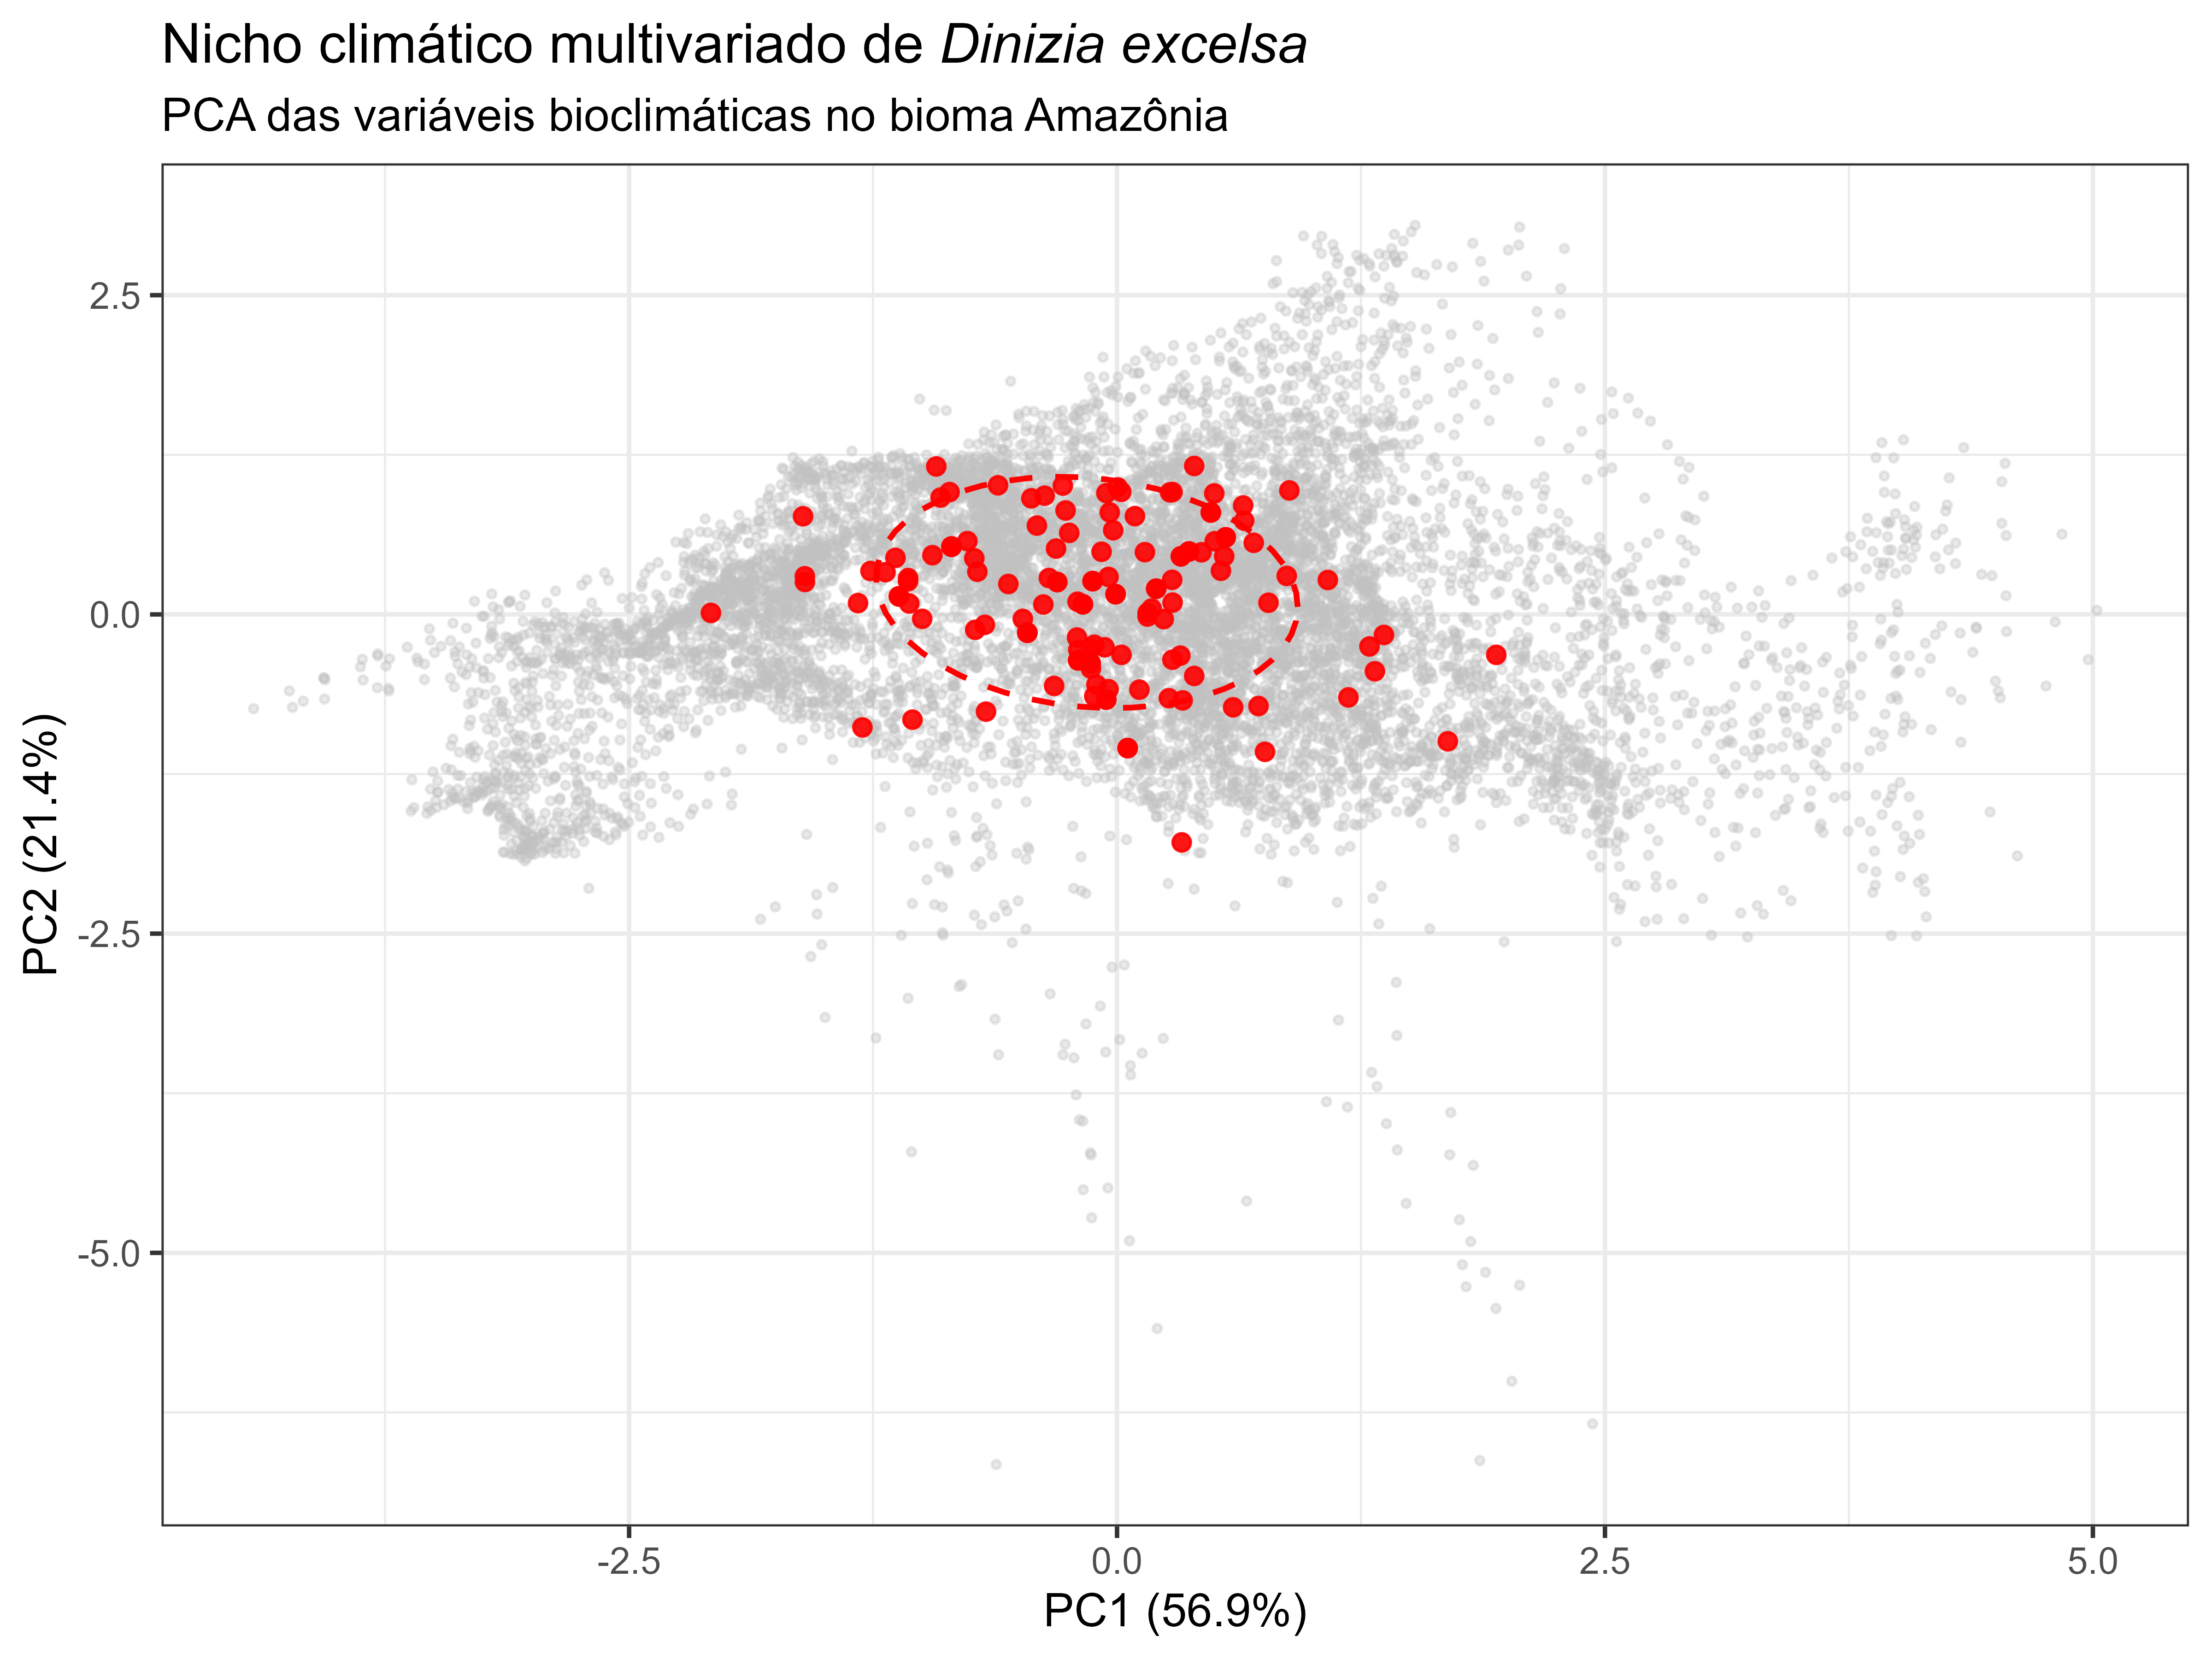
\includegraphics[width=0.85\textwidth]
	{figuras/unidade01/unidade01_pca_nicho_climatico_dinizia.png}
	\caption{
		Representação do nicho climático de \textit{Dinizia excelsa} no espaço ambiental multivariado utilizando Análise de Componentes Principais. Os pontos cinza representam o background climático disponível na Amazônia, enquanto os pontos vermelhos representam as ocorrências observadas da espécie.
	}
	\label{fig:unidade01_pca_nicho}
\end{figure}

Observa-se que as ocorrências de \textit{Dinizia excelsa} ocupam apenas uma fração do conjunto de condições climáticas disponíveis no bioma Amazônia. Esse padrão sugere que a espécie responde a combinações específicas de variáveis ambientais e ilustra de forma prática a ideia de hipervolume ecológico proposta por Hutchinson.

O espaço ambiental ocupado pela espécie representa uma pequena região dentro do universo muito maior de condições disponíveis na Amazônia. A tarefa dos modelos de distribuição consiste justamente em identificar essa região e projetá-la para o espaço geográfico.

A formulação de Hutchinson representa, portanto, a principal base conceitual da moderna Modelagem de Distribuição de Espécies. Entretanto, sua contribuição não se limita à definição do nicho como um hipervolume multidimensional. A partir dessa estrutura teórica surgiram dois conceitos que desempenham papel central na Ecologia contemporânea: o nicho fundamental e o nicho realizado.

Esses conceitos serão discutidos na próxima seção e constituem elementos indispensáveis para compreender o que os modelos de distribuição realmente estimam quando utilizamos registros de ocorrência para inferir padrões ecológicos.

%================================================
\section{Nicho fundamental e nicho realizado}
%================================================

A formulação do nicho ecológico como um hipervolume multidimensional proposta por Hutchinson representou um avanço extraordinário para a Ecologia. Entretanto, uma das contribuições mais influentes de sua teoria não foi apenas a definição matemática do nicho, mas a distinção entre dois conceitos que permanecem centrais para a Ecologia contemporânea e para a Modelagem de Distribuição de Espécies: o nicho fundamental e o nicho realizado \parencite{hutchinson1957}.

Essa distinção é particularmente importante porque permite compreender por que a distribuição observada de uma espécie frequentemente representa apenas uma fração das condições ambientais que ela potencialmente poderia ocupar. Além disso, fornece a base conceitual necessária para interpretar corretamente os resultados produzidos por modelos de distribuição, especialmente quando utilizados para prever áreas potencialmente adequadas sob condições ambientais atuais, passadas ou futuras.

Em termos gerais, o nicho fundamental representa o conjunto completo de condições ambientais sob as quais uma espécie seria capaz de sobreviver, crescer e manter populações viáveis na ausência de restrições impostas por interações ecológicas negativas ou limitações de dispersão. Já o nicho realizado corresponde à porção desse espaço potencial que é efetivamente ocupada pela espécie na natureza.

Essa diferença aparentemente simples possui implicações profundas para a compreensão da distribuição geográfica dos organismos.

\subsection{O nicho fundamental}

O nicho fundamental pode ser definido como o conjunto de todas as combinações ambientais compatíveis com a persistência de uma espécie quando considerados exclusivamente seus limites fisiológicos e ecológicos intrínsecos \parencite{hutchinson1957,pulliam2000}.

Sob essa perspectiva, o nicho fundamental representa o potencial ecológico máximo da espécie. Ele descreve onde a espécie poderia ocorrer se fatores como competição, predação, parasitismo, barreiras geográficas e limitações de dispersão fossem removidos ou não exercessem influência significativa.

Em outras palavras, o nicho fundamental está diretamente relacionado à capacidade fisiológica dos organismos de tolerarem diferentes condições ambientais.

Para plantas, por exemplo, esse espaço pode ser determinado por fatores como tolerância térmica, resistência ao déficit hídrico, capacidade fotossintética, eficiência no uso da água, exigências nutricionais e limites de sobrevivência sob diferentes condições climáticas \parencite{woodward1987,lambers2008}.

Para animais, fatores como temperatura corporal, disponibilidade energética, exigências metabólicas e tolerância a extremos ambientais também contribuem para definir os limites do nicho fundamental \parencite{angilletta2009}.

Do ponto de vista conceitual, o nicho fundamental corresponde ao conjunto de condições ambientais nas quais a taxa de crescimento populacional é positiva ou, pelo menos, suficiente para garantir a persistência da população ao longo do tempo.

\begin{equationbox}
	[
	r > 0
	]
\end{equationbox}

onde (r) representa a taxa intrínseca de crescimento populacional.

Essa interpretação enfatiza que o nicho fundamental não se refere simplesmente à presença de indivíduos, mas à capacidade de manutenção de populações viáveis.

\begin{conceito}
	O nicho fundamental representa o conjunto de condições ambientais sob as quais uma espécie poderia persistir caso apenas seus limites fisiológicos fossem considerados.
\end{conceito}

Embora conceitualmente poderoso, o nicho fundamental é extremamente difícil de estimar diretamente na natureza. Isso ocorre porque os registros de ocorrência disponíveis geralmente já refletem a influência simultânea de múltiplos processos ecológicos e históricos.

Consequentemente, a maioria dos dados utilizados em estudos ecológicos não permite observar diretamente o nicho fundamental, mas apenas suas manifestações sob condições reais de campo.

\subsection{O nicho realizado}

Enquanto o nicho fundamental representa o potencial ecológico da espécie, o nicho realizado corresponde à parcela desse potencial que é efetivamente ocupada na natureza \parencite{hutchinson1957,pulliam2000}.

Na prática, as espécies raramente conseguem ocupar todas as condições ambientalmente adequadas. Diversos processos atuam restringindo a ocupação efetiva do espaço ambiental disponível.

Competidores podem excluir determinadas espécies de habitats potencialmente favoráveis. Predadores e patógenos podem reduzir o sucesso populacional em algumas regiões. Barreiras geográficas podem impedir a colonização de áreas adequadas. Limitações históricas de dispersão podem impedir que espécies alcancem determinados ambientes mesmo após milhares de anos de evolução.

Como consequência, a distribuição observada normalmente representa apenas uma fração do nicho fundamental.

\begin{conceito}
	O nicho realizado corresponde à porção do nicho fundamental efetivamente ocupada pela espécie após a ação de filtros ecológicos, biogeográficos e históricos.
\end{conceito}

Essa diferença entre potencial e ocupação efetiva constitui um dos princípios mais importantes da Ecologia moderna.

Em muitos casos, duas espécies podem apresentar nichos fundamentais semelhantes, mas nichos realizados muito diferentes devido às interações ecológicas estabelecidas em cada região.

Da mesma forma, espécies introduzidas em novas áreas frequentemente passam a ocupar ambientes que não utilizavam em suas regiões nativas. Esse fenômeno pode ocorrer devido à ausência de competidores, predadores ou patógenos que anteriormente restringiam seu nicho realizado \parencite{peterson2011}.

Esses exemplos demonstram que a distribuição observada nem sempre reflete completamente o potencial ecológico da espécie.

\subsection{A relação entre nicho fundamental e nicho realizado}

A relação entre nicho fundamental e nicho realizado pode ser representada conceitualmente como um conjunto de subconjuntos hierárquicos.

O nicho realizado encontra-se contido dentro do nicho fundamental, uma vez que a espécie somente pode ocupar condições compatíveis com sua tolerância fisiológica. Entretanto, nem todas as condições potencialmente adequadas são necessariamente ocupadas.

\begin{figure}[H]
	\centering
	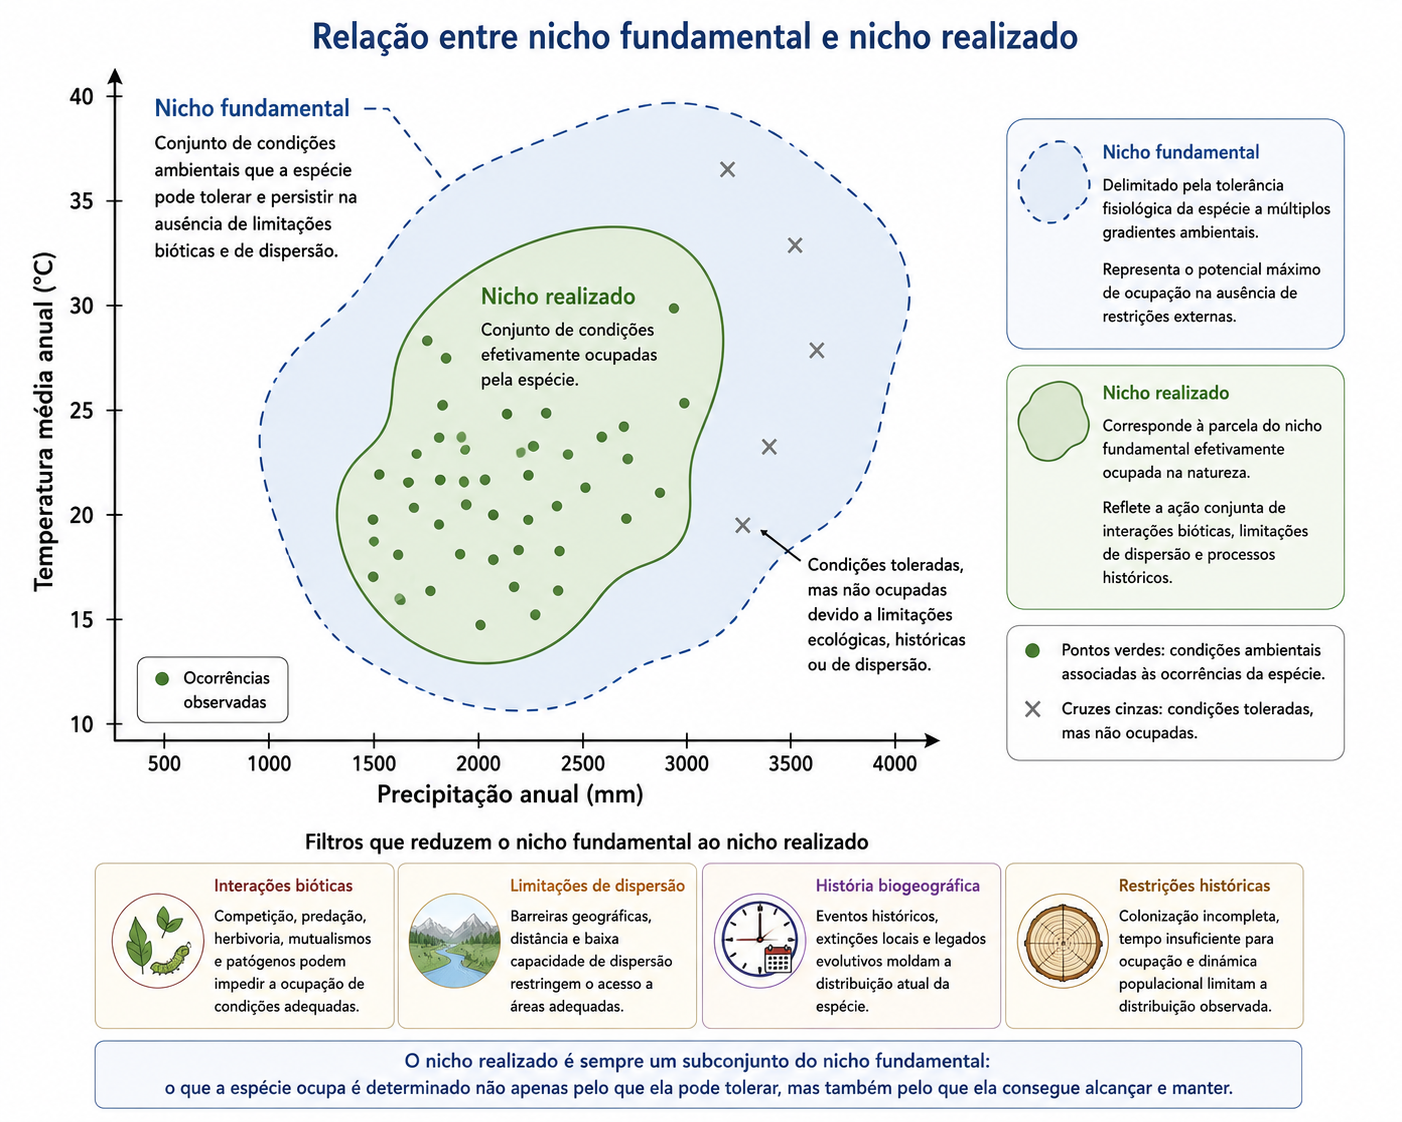
\includegraphics[width=0.75\textwidth]{figuras/unidade01/nicho_fundamental_realizado.png}
	\caption{
		Representação conceitual da relação entre nicho fundamental e nicho realizado. O nicho fundamental corresponde ao conjunto de condições ambientalmente toleradas pela espécie. O nicho realizado representa a parcela efetivamente ocupada após a ação de interações ecológicas, limitações de dispersão e processos históricos.
	}
	\label{fig:nicho_fundamental_realizado}
\end{figure}

A Figura~\ref{fig:nicho_fundamental_realizado} ilustra essa relação. O nicho fundamental representa o potencial fisiológico da espécie, enquanto o nicho realizado corresponde ao subconjunto efetivamente ocupado após a atuação de múltiplos filtros ecológicos.

Essa diferença torna-se particularmente importante em estudos de distribuição geográfica porque os dados de ocorrência disponíveis normalmente representam apenas o nicho realizado.

\subsection{O que os modelos de distribuição realmente estimam?}

Uma das questões mais discutidas na literatura de Modelagem de Distribuição de Espécies refere-se justamente ao tipo de nicho que está sendo representado pelos modelos \parencite{soberon2007,peterson2011,guisan2017habitat}.

Em teoria, muitos pesquisadores gostariam de estimar o nicho fundamental das espécies, pois ele representa o verdadeiro potencial ecológico dos organismos. Entretanto, na prática, a maioria dos modelos correlativos utiliza registros de ocorrência obtidos em condições naturais.

Esses registros já incorporam os efeitos da competição, da dispersão, dos filtros históricos e de inúmeros outros processos ecológicos.

Consequentemente, a maior parte dos modelos correlativos tende a estimar uma aproximação do nicho realizado ou, mais precisamente, da porção do nicho realizado que foi amostrada pelos registros disponíveis \parencite{soberon2007}.

\begin{atencao}
	Um erro comum em SDM é interpretar os modelos como estimativas diretas do nicho fundamental. Na maioria dos casos, os modelos representam apenas uma aproximação do nicho realizado observado sob condições atuais.
\end{atencao}

Essa limitação não invalida os modelos, mas exige cautela em sua interpretação.

Por exemplo, quando um modelo prevê áreas ambientalmente adequadas onde a espécie não ocorre atualmente, isso não significa necessariamente que o modelo esteja errado. A ausência pode refletir limitações de dispersão, barreiras geográficas, histórico evolutivo ou interações ecológicas não representadas pelas variáveis utilizadas.

Da mesma forma, áreas atualmente ocupadas podem tornar-se inadequadas no futuro em função das mudanças climáticas, mesmo que a espécie ainda esteja presente no local devido à longevidade dos indivíduos.

\subsection{Nicho fundamental, nicho realizado e árvores gigantes da Amazônia}

A distinção entre nicho fundamental e nicho realizado possui implicações particularmente relevantes para espécies arbóreas tropicais de grande porte.

Árvores gigantes da Amazônia, como \textit{Dinizia excelsa}, \textit{Bertholletia excelsa}, \textit{Ceiba pentandra} e diversas outras espécies emergentes, apresentam ciclos de vida extremamente longos, frequentemente superiores a vários séculos \parencite{feldpausch2011}.

Como consequência, a distribuição atual dos indivíduos adultos pode refletir condições ambientais existentes durante períodos passados, quando os indivíduos foram recrutados.

Nesse contexto, a presença atual de grandes árvores não garante que as condições ambientais continuem adequadas para a regeneração futura da espécie.

Essa situação pode gerar diferenças importantes entre o nicho observado para indivíduos adultos e o nicho efetivamente necessário para o estabelecimento de novos indivíduos.

Em cenários de mudanças climáticas, essa discrepância pode tornar-se ainda mais relevante. Populações adultas podem persistir durante décadas em áreas que já não oferecem condições ideais para recrutamento, criando uma aparente estabilidade geográfica que mascara processos graduais de declínio populacional.

Por essa razão, estudos modernos de Modelagem de Distribuição de Espécies têm buscado integrar informações demográficas, fisiológicas e ecológicas para produzir representações mais realistas do potencial de persistência das espécies sob condições ambientais futuras.

\subsection{Uma transição para o conceito de distribuição potencial}

A distinção entre nicho fundamental e nicho realizado fornece a base conceitual necessária para compreender outro aspecto fundamental da Modelagem de Distribuição de Espécies: a diferença entre distribuição observada, distribuição real e distribuição potencial.

Enquanto o nicho fundamental descreve as condições sob as quais a espécie poderia persistir e o nicho realizado descreve as condições efetivamente ocupadas, a distribuição potencial representa a projeção espacial dessas relações ecológicas sobre a paisagem.

Compreender essa distinção é essencial para interpretar corretamente mapas de adequabilidade ambiental, projeções climáticas e inferências ecológicas derivadas dos modelos de distribuição.

É justamente essa relação entre nicho e distribuição que será explorada na próxima seção.

%================================================
\section{Distribuição observada, distribuição real e distribuição potencial}
%================================================

Uma das interpretações equivocadas mais frequentes em estudos de Modelagem de Distribuição de Espécies ocorre quando os mapas produzidos pelos modelos são confundidos com a distribuição real das espécies. Embora essa confusão pareça simples, ela possui implicações profundas para a interpretação ecológica dos resultados e pode levar a inferências incorretas sobre conservação, mudanças climáticas, invasões biológicas e planejamento ambiental.

Para compreender adequadamente o que os modelos de distribuição representam, é necessário distinguir três conceitos fundamentais: distribuição observada, distribuição real e distribuição potencial. Esses conceitos estão diretamente relacionados à teoria do nicho ecológico discutida nas seções anteriores e constituem a base para interpretar mapas de adequabilidade ambiental de forma biologicamente consistente.

De maneira geral, a distribuição observada corresponde aos locais onde a espécie foi registrada; a distribuição real corresponde aos locais efetivamente ocupados pela espécie na natureza; e a distribuição potencial corresponde ao conjunto de áreas que apresentam condições ambientalmente adequadas para sua ocorrência, independentemente de estarem atualmente ocupadas.

Embora esses conceitos estejam relacionados, eles não são equivalentes e frequentemente apresentam diferenças substanciais na prática.

\subsection{Distribuição observada: o que realmente conhecemos}

A distribuição observada corresponde ao conjunto de registros disponíveis para uma espécie em determinado momento. Esses registros podem ser obtidos a partir de herbários, coleções zoológicas, inventários florestais, levantamentos de campo, monitoramentos ecológicos, literatura científica ou plataformas globais de biodiversidade, como GBIF, SpeciesLink e iNaturalist \parencite{hijmans2021,gbif2024}.

Na maioria dos estudos de Modelagem de Distribuição de Espécies, os registros de ocorrência constituem o principal ponto de partida para a construção dos modelos. São esses dados que permitem associar a presença da espécie às condições ambientais existentes nos locais onde ela foi observada.

Entretanto, é importante reconhecer que a distribuição observada representa apenas uma amostra do conhecimento disponível sobre a ocorrência da espécie.

\begin{conceito}
	A distribuição observada corresponde ao conjunto de registros conhecidos da espécie, obtidos por meio de amostragens, coleções biológicas, inventários ou observações documentadas.
\end{conceito}

Essa definição possui uma consequência importante: a distribuição observada depende diretamente do esforço amostral realizado.

Espécies amplamente estudadas tendem a possuir milhares de registros distribuídos por diferentes regiões. Em contraste, espécies raras, pouco conhecidas ou associadas a ambientes de difícil acesso frequentemente apresentam poucos registros disponíveis, mesmo quando ocupam áreas extensas.

Essa limitação é particularmente relevante em regiões tropicais.

Na Amazônia, por exemplo, vastas áreas permanecem biologicamente subamostradas devido às dificuldades logísticas, aos elevados custos operacionais e à limitada infraestrutura de pesquisa em algumas regiões. Como consequência, muitas espécies apresentam registros concentrados próximos a rios navegáveis, estradas, centros urbanos, estações de pesquisa ou unidades de conservação mais acessíveis \parencite{nelson1990,feeley2005}.

Esses padrões de amostragem geram os chamados vieses espaciais de ocorrência, considerados uma das principais fontes de incerteza em Modelagem de Distribuição de Espécies \parencite{phillips2009,viera2022}.

A Figura~\ref{fig:unidade01_ocorrencias_dinizia} ilustra esse conceito utilizando registros de ocorrência de \textit{Dinizia excelsa} distribuídos no bioma Amazônia.

\begin{figure}[H]
	\centering
	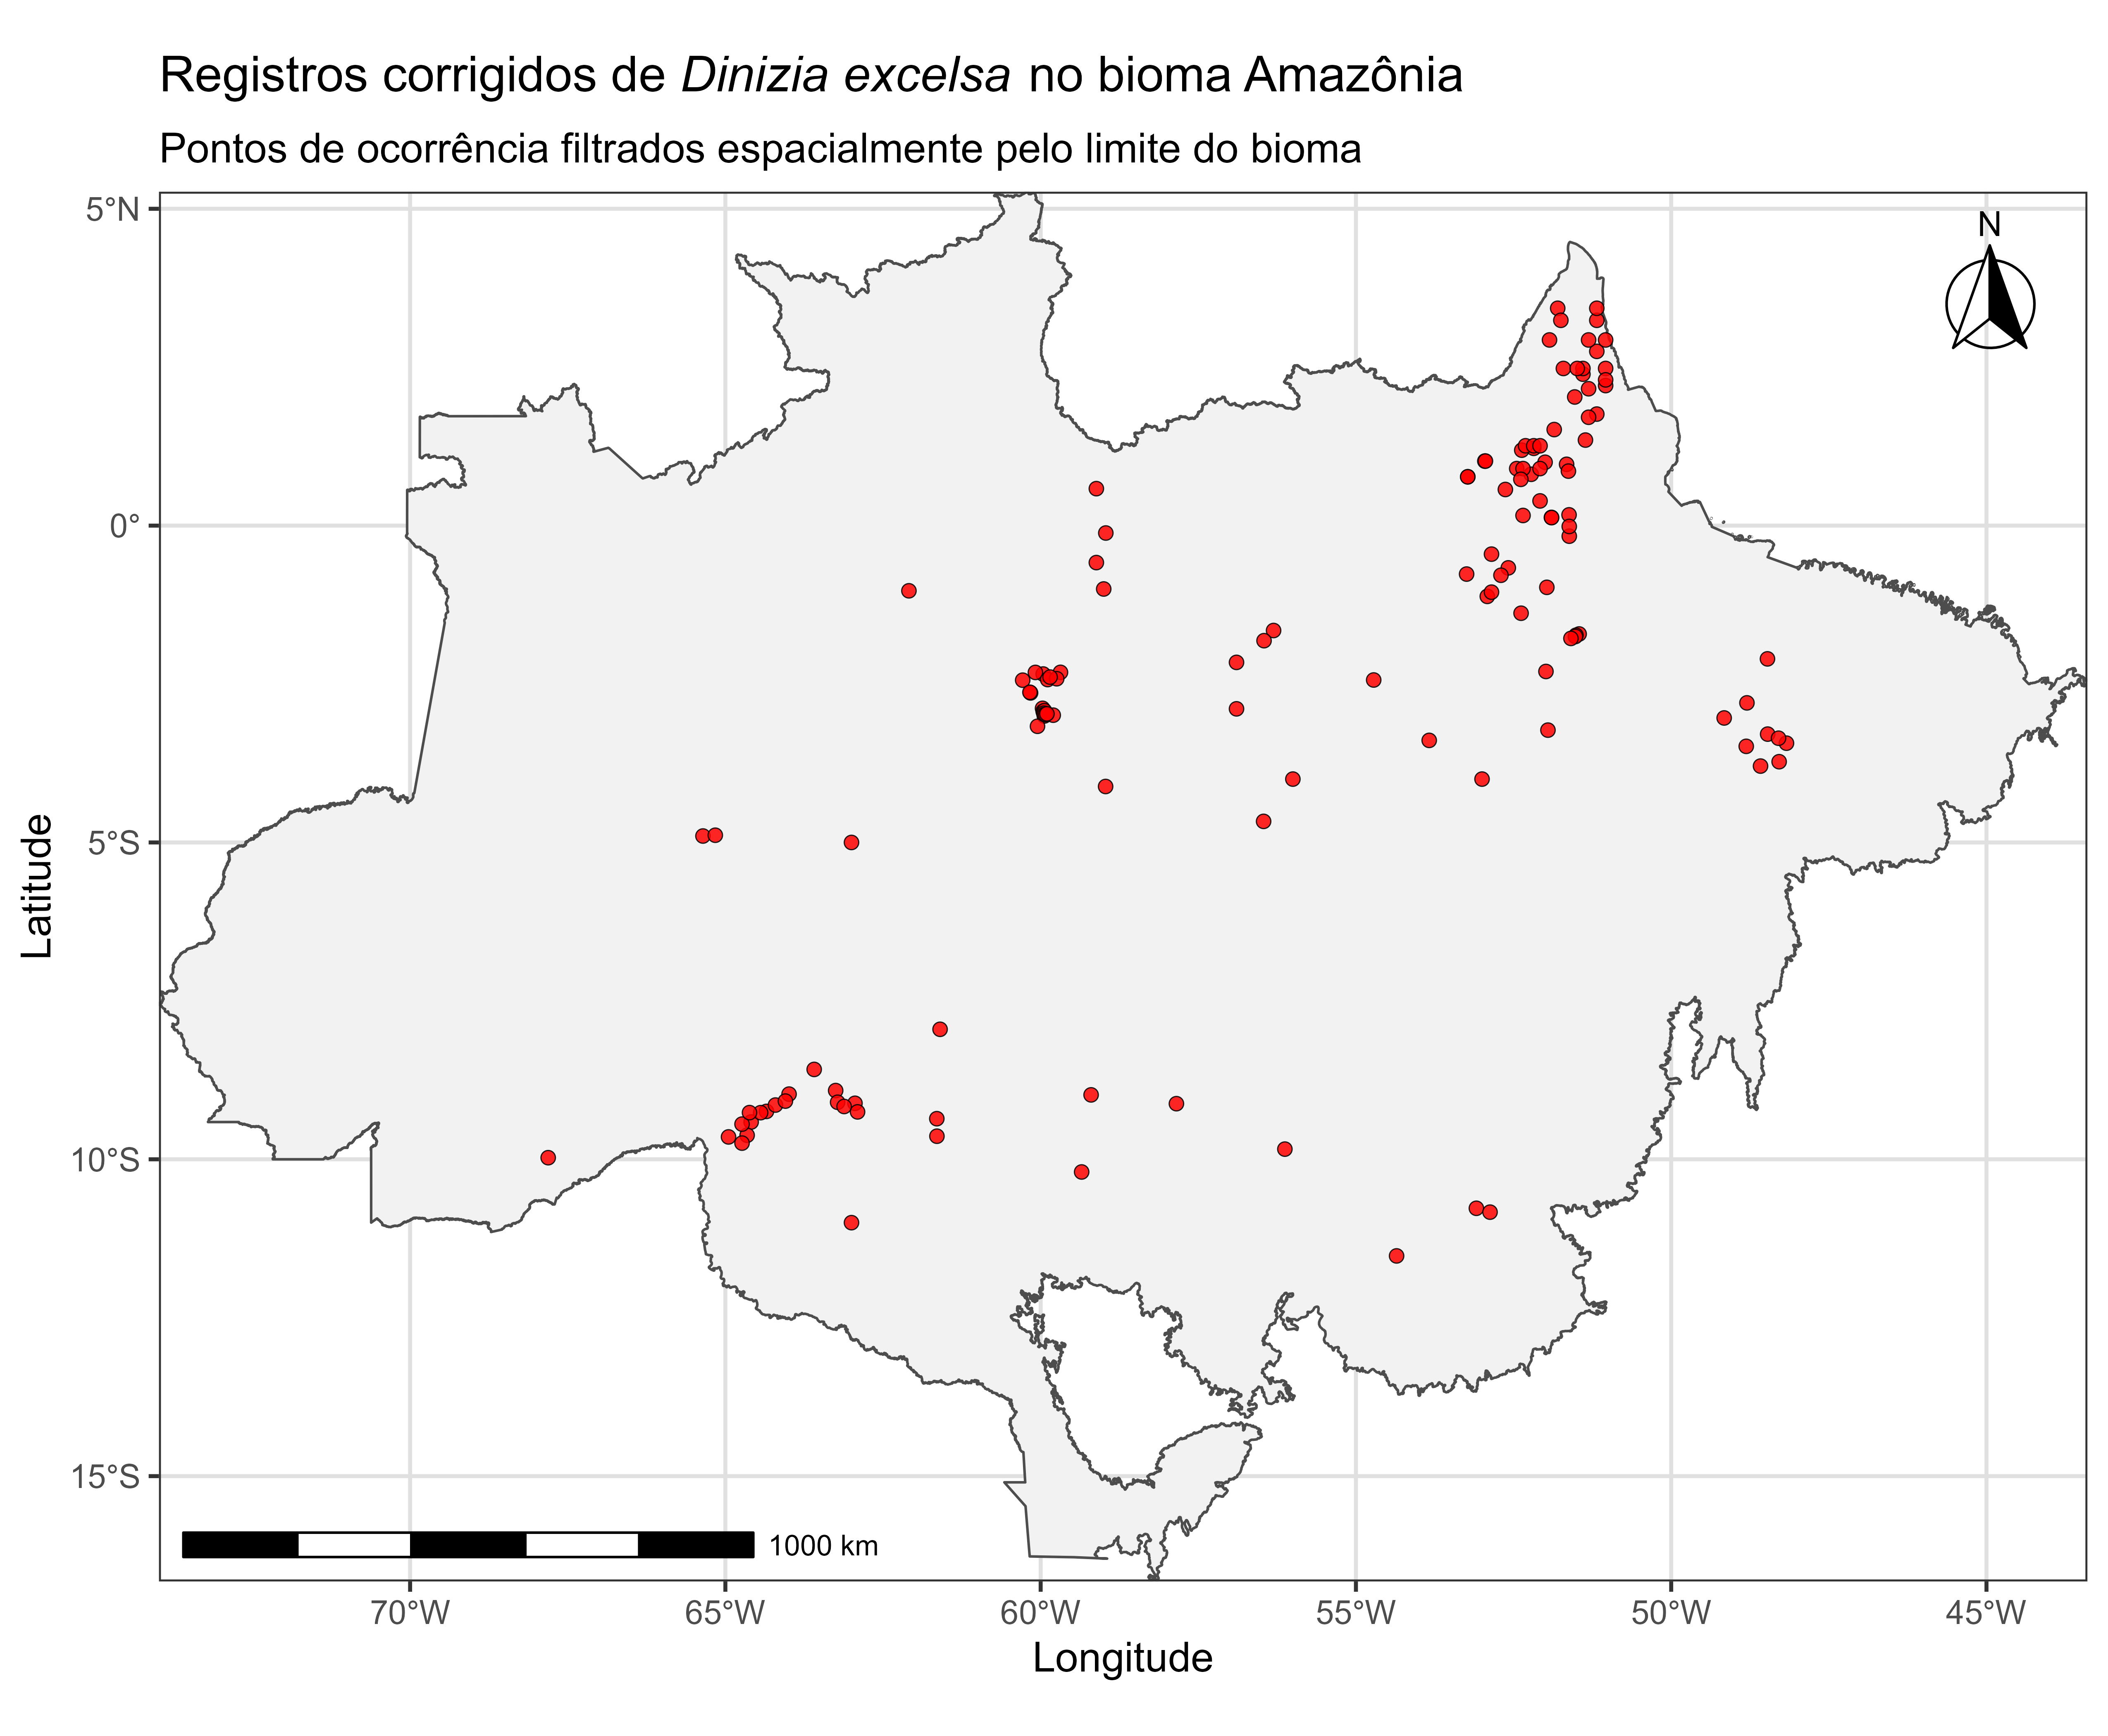
\includegraphics[width=0.85\textwidth]
	{figuras/unidade01/unidade01_mapa_ocorrencias_dinizia.png}
	\caption{
		Distribuição observada de \textit{Dinizia excelsa} no bioma Amazônia após procedimentos de limpeza taxonômica, remoção de duplicatas e filtragem espacial. Os pontos representam registros documentados da espécie e constituem uma amostra da distribuição conhecida disponível para análise.
	}
	\label{fig:unidade01_ocorrencias_dinizia}
\end{figure}

Observa-se que os registros encontram-se distribuídos de forma heterogênea ao longo da Amazônia. Essa distribuição espacial reflete simultaneamente processos ecológicos reais e padrões históricos de amostragem.

Consequentemente, a ausência de registros em determinada região não deve ser interpretada automaticamente como ausência da espécie.

\begin{atencao}
	Ausência de registros não é sinônimo de ausência ecológica. Em muitos casos, ela simplesmente reflete ausência de amostragem adequada.
\end{atencao}

Essa distinção constitui uma das justificativas fundamentais para o desenvolvimento dos modelos de distribuição.

\subsection{Distribuição real: a ocupação efetiva da espécie}

A distribuição real corresponde ao conjunto de locais efetivamente ocupados pela espécie em determinado período de tempo, independentemente de esses locais terem sido amostrados ou documentados \parencite{gaston2003}.

Em teoria, a distribuição real representa a verdadeira extensão geográfica da espécie na natureza. Entretanto, sua determinação exata é praticamente impossível para a maioria dos organismos.

Mesmo espécies relativamente bem estudadas raramente possuem cobertura amostral suficiente para identificar todos os locais onde ocorrem.

Em ecossistemas megadiversos, como a Amazônia, esse desafio torna-se ainda maior. A combinação entre grandes extensões territoriais, elevada riqueza de espécies e limitações logísticas faz com que a distribuição real permaneça desconhecida para grande parte da biodiversidade regional.

Do ponto de vista conceitual, a distribuição real situa-se entre a distribuição observada e a distribuição potencial.

\begin{equationbox}
	[
	Distribuição\ Observada \subseteq Distribuição\ Real
	]
\end{equationbox}

Essa relação indica que os registros observados representam apenas uma parcela dos locais efetivamente ocupados pela espécie.

Quanto maior o esforço amostral, maior tende a ser a aproximação entre distribuição observada e distribuição real. Entretanto, para a maioria das espécies, especialmente em regiões tropicais, essa correspondência permanece incompleta.

\subsection{Distribuição potencial: onde a espécie poderia ocorrer}

O conceito de distribuição potencial emerge diretamente da teoria do nicho ecológico.

Se uma espécie possui determinados requisitos ambientais para sobreviver e se reproduzir, então todas as regiões que apresentam condições compatíveis com esses requisitos podem ser consideradas potencialmente adequadas para sua ocorrência \parencite{peterson2011,franklin2010}.

A distribuição potencial corresponde justamente à projeção espacial dessas condições adequadas.

\begin{conceito}
	A distribuição potencial representa o conjunto de áreas que apresentam condições ambientais compatíveis com o nicho ecológico estimado para a espécie, independentemente de estarem atualmente ocupadas.
\end{conceito}

Diferentemente da distribuição observada, que depende diretamente dos registros disponíveis, a distribuição potencial é inferida por meio de modelos ecológicos.

Os algoritmos utilizam os registros conhecidos para identificar associações entre ocorrência e ambiente. Posteriormente, essas relações são projetadas para toda a paisagem, permitindo estimar quais regiões apresentam condições semelhantes às observadas nos locais de ocorrência.

Essa lógica constitui a essência da Modelagem de Distribuição de Espécies.

A distribuição potencial não descreve necessariamente onde a espécie ocorre atualmente. Ela descreve onde a espécie poderia ocorrer caso as condições ambientais sejam compatíveis e outros fatores limitantes não impeçam sua presença.

Por essa razão, áreas potencialmente adequadas podem permanecer desocupadas devido a limitações de dispersão, barreiras geográficas, eventos históricos ou interações ecológicas não representadas pelo modelo.

\subsection{A relação entre nicho ecológico e distribuição potencial}

A distribuição potencial pode ser interpretada como uma manifestação espacial do nicho ecológico.

Enquanto o nicho é definido no espaço ambiental, a distribuição potencial corresponde à projeção desse nicho sobre o espaço geográfico.

Essa relação pode ser representada de forma simplificada como:

\begin{center}
	Nicho Ecológico
	$\rightarrow$
	Espaço Ambiental
	$\rightarrow$
	Projeção Espacial
	$\rightarrow$
	Distribuição Potencial
\end{center}

Os modelos de distribuição funcionam exatamente segundo essa lógica.

Primeiro, identificam o nicho ecológico utilizando os registros de ocorrência e as variáveis ambientais. Em seguida, projetam essas relações para toda a região de interesse, produzindo mapas de adequabilidade ambiental.

Esses mapas representam aproximações da distribuição potencial da espécie.

\subsection{Um exemplo utilizando \textit{Dinizia excelsa}}

Os conceitos discutidos podem ser ilustrados utilizando o estudo de caso desenvolvido nesta unidade.

A Figura~\ref{fig:unidade01_nicho_tp_dinizia} apresenta a distribuição das ocorrências de \textit{Dinizia excelsa} em relação ao espaço climático disponível na Amazônia.

\begin{figure}[H]
	\centering
	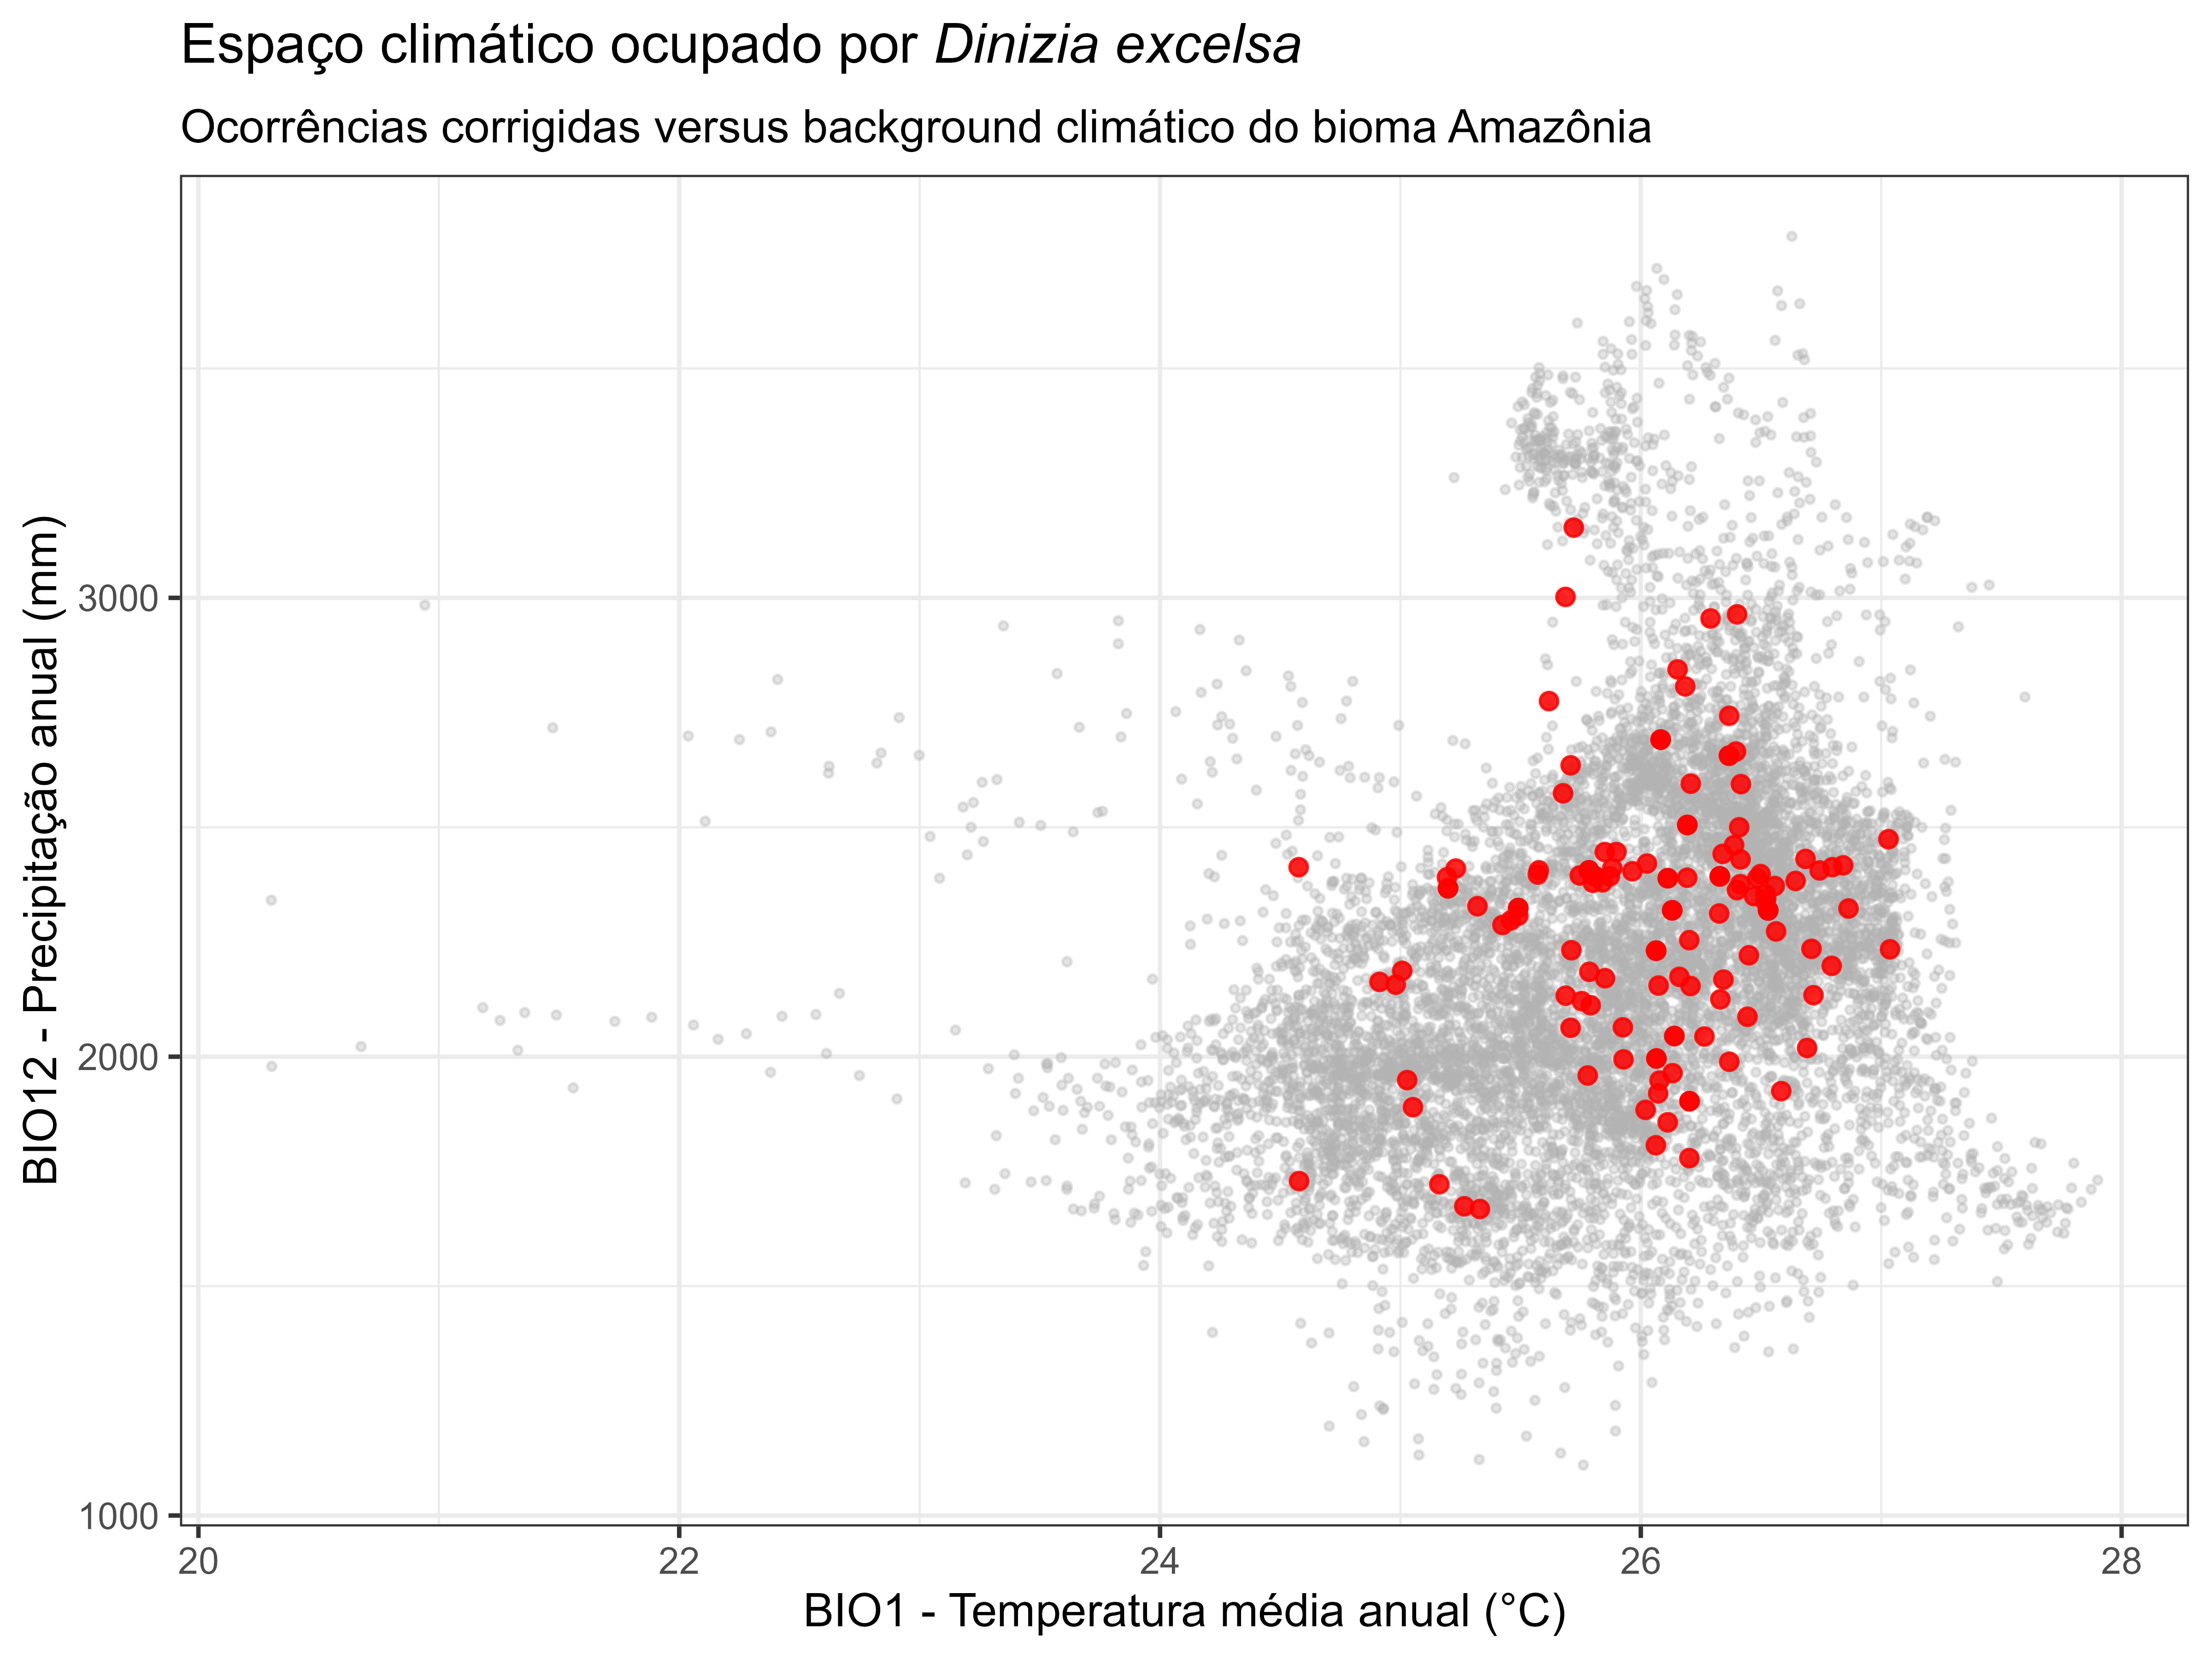
\includegraphics[width=0.85\textwidth]
	{figuras/unidade01/unidade01_nicho_temperatura_precipitacao_dinizia.png}
	\caption{
		Espaço climático ocupado por \textit{Dinizia excelsa} em relação ao conjunto de condições ambientais disponíveis no bioma Amazônia. Os pontos vermelhos representam ocorrências observadas e os pontos cinza representam o background ambiental disponível.
	}
	\label{fig:unidade01_nicho_tp_dinizia}
\end{figure}

Observa-se que as ocorrências conhecidas ocupam apenas uma fração das combinações climáticas disponíveis.

Essa informação permite inferir quais condições ambientais estão associadas à presença da espécie e constitui a base para estimar sua distribuição potencial.

Nas unidades posteriores, esses mesmos princípios serão utilizados para construir modelos capazes de gerar mapas contínuos de adequabilidade ambiental, identificar áreas prioritárias para conservação e projetar possíveis alterações na distribuição da espécie sob diferentes cenários climáticos.

\subsection{Implicações para a interpretação de mapas de adequabilidade}

Um dos erros mais comuns em SDM consiste em interpretar mapas de adequabilidade ambiental como mapas de presença e ausência.

Na realidade, a maioria dos modelos produz superfícies contínuas que representam gradientes de adequabilidade ou suporte ambiental à ocorrência da espécie \parencite{elith2009,guisan2017habitat}.

Valores elevados indicam que as condições ambientais são semelhantes àquelas observadas nos locais onde a espécie ocorre. Valores baixos indicam menor similaridade ambiental.

Entretanto, esses valores não representam diretamente abundância populacional, densidade de indivíduos ou probabilidade verdadeira de ocorrência.

\begin{atencao}
	Mapas de adequabilidade ambiental devem ser interpretados como hipóteses ecológicas espacialmente explícitas sobre a relação entre espécie e ambiente, e não como representações exatas da distribuição real.
\end{atencao}

Essa interpretação é particularmente importante quando os modelos são utilizados para apoiar decisões de conservação, planejamento territorial ou projeções sob mudanças climáticas.

Compreender as diferenças entre distribuição observada, distribuição real e distribuição potencial permite reconhecer tanto o poder quanto as limitações da Modelagem de Distribuição de Espécies.

Esses conceitos também fornecem a base necessária para compreender um dos pressupostos mais importantes das projeções ecológicas modernas: a hipótese de conservação de nicho, tema que será discutido na próxima seção.

%================================================
\section{Conservação de nicho}
%================================================

A conservação de nicho constitui um dos conceitos mais importantes para a Modelagem de Distribuição de Espécies, especialmente quando os modelos são utilizados para realizar projeções espaciais ou temporais. Em termos gerais, a conservação de nicho refere-se à tendência de espécies, populações ou linhagens manterem ao longo do tempo requisitos ambientais semelhantes aos de seus ancestrais ou populações de origem \parencite{peterson1999,wiens2010}.

Essa ideia é central porque muitos estudos de SDM dependem implicitamente da suposição de que a relação observada entre espécie e ambiente no presente permanecerá suficientemente estável para ser projetada para outros períodos, regiões ou cenários ambientais. Quando um modelo calibrado com dados atuais é projetado para o futuro, assume-se que a espécie continuará respondendo de forma semelhante aos gradientes ambientais utilizados na modelagem \parencite{peterson2011}.

A mesma lógica é aplicada em estudos de paleodistribuição, nos quais modelos calibrados no presente são projetados para períodos passados, como o Último Máximo Glacial ou o Holoceno Médio. Também é aplicada em estudos de invasões biológicas, nos quais ocorrências da área nativa são utilizadas para estimar regiões potencialmente adequadas em áreas introduzidas \parencite{guisan2017habitat}.

\begin{conceito}
	A conservação de nicho é a hipótese de que uma espécie mantém, ao longo do tempo ou entre regiões, relações ambientais suficientemente semelhantes para permitir a transferência espacial ou temporal de modelos de distribuição.
\end{conceito}

A conservação de nicho não significa que o nicho ecológico seja absolutamente fixo ou imutável. Espécies podem apresentar plasticidade fenotípica, adaptação local, expansão de nicho, contração de nicho ou mudança nas condições ocupadas ao longo do tempo. No entanto, para muitas escalas ecológicas e biogeográficas, os requisitos ambientais das espécies tendem a apresentar certo grau de estabilidade, permitindo inferências úteis sobre sua distribuição potencial \parencite{wiens2010,peterson2011}.

Essa distinção é fundamental. A conservação de nicho deve ser compreendida como uma hipótese ecológica testável, e não como uma regra universal. Em algumas situações, a suposição de estabilidade do nicho pode ser razoável; em outras, pode ser inadequada ou exigir avaliação cuidadosa.

\subsection{Por que a conservação de nicho é essencial em SDM?}

A importância da conservação de nicho torna-se evidente quando consideramos o uso dos modelos de distribuição para além da descrição da distribuição atual.

Se um modelo fosse utilizado apenas para interpolar a adequabilidade ambiental dentro da mesma região, período climático e domínio ambiental em que foi calibrado, a necessidade de pressupor conservação de nicho seria relativamente menor. Entretanto, grande parte das aplicações de SDM envolve extrapolação para novos contextos.

Isso ocorre em pelo menos três situações principais:

\begin{enumerate}
	
	\item projeções para cenários climáticos futuros;
	
	\item reconstruções paleoclimáticas e inferências históricas;
	
	\item estimativas de distribuição potencial em regiões não ocupadas ou invadidas.
	
\end{enumerate}

Em todas essas aplicações, o modelo é transferido para condições diferentes daquelas observadas durante sua calibração. Essa transferência somente possui sentido ecológico se a relação entre espécie e ambiente for suficientemente conservada.

Por exemplo, ao projetar a distribuição potencial de uma árvore amazônica para 2050 ou 2070 sob cenários de mudanças climáticas, assume-se que suas respostas às variáveis ambientais selecionadas permanecerão relativamente semelhantes durante esse período. Se a espécie evoluir rapidamente, alterar suas tolerâncias ambientais ou modificar fortemente suas interações ecológicas, a validade da projeção poderá ser reduzida.

\begin{atencao}
	Toda projeção temporal em SDM é condicional. Ela não afirma que a espécie necessariamente ocorrerá em determinada área no futuro, mas indica quais regiões poderão apresentar condições ambientais semelhantes às associadas à espécie no presente, caso a relação espécie--ambiente permaneça conservada.
\end{atencao}

Essa interpretação evita um erro comum: tratar mapas futuros como previsões determinísticas. Em realidade, projeções futuras devem ser entendidas como cenários ecológicos condicionais, dependentes de pressupostos sobre clima, dispersão, persistência populacional, interações bióticas e conservação de nicho.

\subsection{Conservação, mudança e expansão de nicho}

Embora a conservação de nicho seja frequentemente assumida em estudos de SDM, ela não deve ser tratada como inevitável. O nicho ecológico pode apresentar diferentes trajetórias ao longo do tempo ou entre regiões.

Em alguns casos, há forte conservação. A espécie ocupa ambientes semelhantes em diferentes partes de sua distribuição, sugerindo estabilidade de suas tolerâncias ambientais. Em outros casos, ocorre expansão de nicho, quando a espécie passa a ocupar condições ambientais que não utilizava anteriormente. Também pode ocorrer contração de nicho, quando a espécie ocupa apenas parte das condições potencialmente adequadas, possivelmente devido a restrições históricas, dispersão limitada ou interações ecológicas \parencite{broennimann2007,guisan2014}.

Essas mudanças são particularmente discutidas em estudos de invasões biológicas. Espécies introduzidas em novas regiões podem ocupar condições climáticas semelhantes às de sua área nativa, sugerindo conservação de nicho. Entretanto, algumas espécies invadem ambientes climaticamente distintos, indicando possível expansão de nicho ou liberação de restrições bióticas existentes na área original \parencite{broennimann2007}.

A interpretação desses padrões exige cautela. Mudanças aparentes de nicho podem refletir adaptação evolutiva, plasticidade fenotípica, diferenças na disponibilidade ambiental, viés amostral ou ausência de interações ecológicas que limitavam a espécie em sua área nativa \parencite{guisan2014}.

Assim, avaliar conservação de nicho não consiste apenas em comparar mapas de distribuição. É necessário comparar o espaço ambiental ocupado pela espécie em diferentes regiões ou períodos, considerando também o ambiente disponível em cada contexto.

\subsection{Conservação de nicho e mudanças climáticas}

Em estudos de mudanças climáticas, a conservação de nicho desempenha papel central porque permite projetar modelos calibrados sob condições atuais para cenários futuros. Essa abordagem é amplamente utilizada para estimar possíveis perdas, ganhos ou deslocamentos de áreas climaticamente adequadas para espécies e ecossistemas \parencite{thuiller2005,araújo2006}.

A lógica é relativamente simples: se a espécie ocupa atualmente determinado conjunto de condições climáticas, então regiões que apresentarem condições semelhantes no futuro poderão ser consideradas potencialmente adequadas. Da mesma forma, regiões que deixarem de apresentar essas condições poderão tornar-se menos adequadas.

Contudo, essa interpretação deve considerar que espécies diferem fortemente em sua capacidade de acompanhar mudanças climáticas. Organismos com alta mobilidade podem deslocar suas distribuições mais rapidamente, enquanto árvores tropicais de grande porte dependem de processos lentos de dispersão, estabelecimento e crescimento populacional.

No caso de espécies arbóreas amazônicas, essa limitação é particularmente relevante. Mesmo que novas áreas se tornem climaticamente adequadas no futuro, a colonização efetiva poderá ser limitada pela dispersão de sementes, fragmentação da paisagem, disponibilidade de polinizadores e tempo necessário para o estabelecimento de populações reprodutivas.

Por outro lado, áreas atualmente ocupadas podem permanecer com indivíduos adultos por longos períodos mesmo após se tornarem climaticamente inadequadas para o recrutamento. Esse fenômeno pode gerar defasagens temporais entre mudança ambiental e resposta populacional.

\begin{aplicacao}
	Para árvores gigantes da Amazônia, projeções climáticas devem ser interpretadas como estimativas de adequabilidade ambiental, e não como previsões diretas de presença futura. A longevidade dos indivíduos, a limitação de dispersão e a dependência de condições adequadas para regeneração tornam a resposta populacional às mudanças climáticas potencialmente lenta e defasada.
\end{aplicacao}

Essa discussão é essencial para evitar interpretações excessivamente simplificadas de mapas futuros. Uma área projetada como adequada em 2070 pode não ser ocupada pela espécie se houver barreiras de dispersão. Da mesma forma, uma área projetada como inadequada pode ainda conter indivíduos adultos remanescentes, mesmo que a regeneração esteja comprometida.

\subsection{Conservação de nicho e paleoclima}

A conservação de nicho também é fundamental em estudos paleoclimáticos. Quando modelos calibrados no presente são projetados para períodos passados, como o Último Interglacial, o Último Máximo Glacial ou o Holoceno Médio, assume-se que as relações ambientais da espécie permaneceram suficientemente semelhantes ao longo do tempo para permitir inferência histórica \parencite{nogués-bravo2009}.

Essa abordagem permite investigar hipóteses sobre refúgios climáticos, estabilidade histórica, rotas de expansão pós-glacial e mudanças na distribuição potencial das espécies ao longo de milhares de anos.

Em florestas tropicais, estudos paleoclimáticos são particularmente importantes porque ajudam a compreender como oscilações climáticas passadas podem ter influenciado padrões atuais de diversidade, endemismo e estrutura genética das populações.

Entretanto, quanto maior a distância temporal entre o período de calibração e o período de projeção, maior tende a ser a incerteza associada à suposição de conservação de nicho. Mudanças evolutivas, extinções locais, alterações na composição das comunidades e diferenças nas condições ambientais disponíveis podem afetar a interpretação dos resultados.

Por isso, projeções paleoclimáticas devem ser interpretadas como hipóteses históricas compatíveis com o nicho climático atual, e não como reconstruções definitivas da distribuição passada.

\subsection{A conservação de nicho como hipótese testável}

Um ponto essencial é reconhecer que a conservação de nicho não deve ser simplesmente assumida. Sempre que possível, ela deve ser avaliada empiricamente.

Existem diferentes abordagens para testar ou explorar a conservação de nicho. Uma delas consiste em comparar o espaço ambiental ocupado pela espécie em diferentes regiões, períodos ou populações. Outra abordagem envolve projetar modelos calibrados em uma região para outra e avaliar seu desempenho preditivo. Também podem ser utilizados métodos de equivalência e similaridade de nicho, que comparam se dois conjuntos de ocorrências ocupam regiões semelhantes no espaço ambiental \parencite{broennimann2012,warren2008}.

Essas análises permitem distinguir, ainda que parcialmente, casos de conservação, expansão ou deslocamento de nicho.

No entanto, é importante lembrar que a interpretação desses testes depende fortemente da qualidade dos dados de ocorrência, da seleção das variáveis ambientais, da delimitação da área acessível e da representatividade do background ambiental utilizado.

\begin{atencao}
	Testes de conservação de nicho são sensíveis ao ambiente disponível. Comparar nichos sem considerar diferenças no background ambiental pode levar a conclusões equivocadas sobre mudança ou estabilidade de nicho.
\end{atencao}

Essa observação conecta diretamente a conservação de nicho ao conceito de área acessível (M), que será discutido em profundidade nas próximas unidades. A delimitação inadequada do ambiente disponível pode gerar interpretações artificiais de expansão ou contração de nicho.

\subsection{Implicações para o estudo de \textit{Dinizia excelsa}}

No contexto deste livro, a hipótese de conservação de nicho será particularmente importante porque os modelos ajustados para \textit{Dinizia excelsa} serão posteriormente projetados para cenários climáticos futuros e paleoclimáticos.

A espécie é uma árvore amazônica de grande porte, e sua distribuição atual provavelmente reflete tanto condições climáticas contemporâneas quanto processos históricos de dispersão, dinâmica florestal e persistência populacional. Assim, ao utilizar modelos para inferir áreas adequadas sob diferentes períodos, assume-se que parte importante de suas exigências climáticas permanece conservada.

Essa suposição é plausível como ponto de partida, mas não deve ser interpretada como certeza absoluta. A longevidade dos indivíduos, a possível defasagem entre ocorrência adulta e regeneração, a influência de eventos climáticos extremos e as interações ecológicas locais podem modificar a relação entre adequabilidade climática e persistência populacional.

Portanto, as projeções futuras e paleoclimáticas apresentadas nas unidades posteriores deverão ser interpretadas como cenários de adequabilidade ambiental sob a hipótese de conservação parcial do nicho climático.

\subsection{Síntese da seção}

A conservação de nicho é um pressuposto central para a transferência espacial e temporal de modelos de distribuição. Ela permite projetar relações espécie--ambiente para novos períodos, regiões ou cenários climáticos, mas deve ser interpretada como uma hipótese ecológica condicional.

Quando bem compreendida, a conservação de nicho fortalece a interpretação dos modelos e torna explícitas suas premissas. Quando ignorada, pode levar à interpretação equivocada de mapas de adequabilidade como previsões determinísticas da presença futura ou passada das espécies.

Essa discussão prepara o caminho para compreender como mudanças climáticas podem alterar a distribuição espacial das condições ambientais que compõem o nicho ecológico das espécies, tema abordado na próxima seção.

%================================================
\section{Nicho ecológico e mudanças climáticas}
%================================================

As mudanças climáticas globais representam uma das principais forças contemporâneas capazes de modificar a distribuição geográfica das espécies. Ao alterar gradientes de temperatura, precipitação, sazonalidade, disponibilidade hídrica e frequência de eventos extremos, as mudanças climáticas modificam diretamente a distribuição espacial das condições ambientais que compõem o nicho ecológico dos organismos \parencite{parmesan2006,ipcc2021}.

Essa relação torna o conceito de nicho ecológico indispensável para compreender os possíveis efeitos das mudanças climáticas sobre a biodiversidade. Se a ocorrência de uma espécie depende de determinadas combinações ambientais, qualquer alteração persistente nessas condições pode modificar a extensão, a localização e a conectividade das áreas adequadas para sua persistência \parencite{thuiller2005,araújo2006}.

Em termos conceituais, as mudanças climáticas não deslocam diretamente as espécies. O que se desloca inicialmente é o espaço ambiental adequado. As populações somente acompanharão esse deslocamento se forem capazes de dispersar, estabelecer novos indivíduos, manter interações ecológicas essenciais e persistir diante das novas condições ambientais.

Essa distinção é fundamental para interpretar corretamente projeções de distribuição futura.

\begin{conceito}
	Mudanças climáticas alteram a distribuição geográfica das condições ambientais que compõem o nicho ecológico. A resposta das espécies dependerá de sua capacidade de acompanhar, tolerar ou persistir diante dessas mudanças.
\end{conceito}

\subsection{Do deslocamento climático ao deslocamento da adequabilidade ambiental}

Quando a temperatura média aumenta ou o regime de precipitação se modifica, regiões anteriormente adequadas podem deixar de apresentar condições compatíveis com o nicho da espécie. Da mesma forma, áreas que antes eram frias, secas ou sazonalmente desfavoráveis podem passar a apresentar condições mais próximas daquelas atualmente ocupadas pela espécie.

Esse processo é frequentemente descrito como deslocamento climático do nicho. Entretanto, é mais preciso afirmar que ocorre uma redistribuição espacial da adequabilidade ambiental \parencite{guisan2017habitat}.

Em Modelagem de Distribuição de Espécies, essa redistribuição é estimada por meio da projeção de modelos calibrados no presente para cenários climáticos futuros. A lógica é direta: se o modelo identifica as condições climáticas associadas à ocorrência atual da espécie, então é possível projetar onde essas condições poderão ocorrer no futuro sob diferentes cenários de emissão de gases de efeito estufa.

No entanto, essa projeção depende de pressupostos importantes. O principal deles é a conservação parcial do nicho climático. Assume-se que a relação entre ocorrência e ambiente estimada no presente permanecerá suficientemente válida durante o período projetado \parencite{peterson2011}.

Essa suposição não deve ser interpretada como garantia de previsão. Projeções futuras representam cenários condicionais e devem ser compreendidas como hipóteses espacialmente explícitas sobre a redistribuição potencial da adequabilidade ambiental.

\begin{atencao}
	Mapas futuros de adequabilidade não indicam onde a espécie certamente ocorrerá. Eles indicam onde as condições ambientais poderão se tornar mais ou menos semelhantes àquelas atualmente associadas à ocorrência da espécie.
\end{atencao}

Essa interpretação é especialmente importante para espécies com baixa capacidade de dispersão, longos ciclos de vida ou forte dependência de interações ecológicas específicas.

\subsection{Ganhos, perdas e estabilidade climática}

As projeções de distribuição futura geralmente são interpretadas a partir de três componentes principais: perda de adequabilidade, ganho de adequabilidade e estabilidade climática.

As áreas de perda correspondem a regiões atualmente adequadas que se tornam inadequadas no futuro. Essas áreas podem indicar regiões onde populações existentes estarão potencialmente expostas a condições ambientais desfavoráveis.

As áreas de ganho correspondem a regiões atualmente inadequadas que se tornam adequadas em cenários futuros. Contudo, a interpretação dessas áreas exige cautela, pois adequabilidade climática futura não implica ocupação efetiva. Para que a espécie colonize essas áreas, será necessário que exista conectividade, capacidade de dispersão, disponibilidade de habitat e ausência de barreiras ecológicas relevantes.

As áreas estáveis correspondem a regiões que permanecem adequadas entre o presente e o futuro. Em estudos de conservação, essas áreas são frequentemente interpretadas como potenciais refúgios climáticos, pois podem oferecer maior continuidade ambiental para populações ao longo do tempo \parencite{ashcroft2010}.

\begin{conceito}
	Áreas estáveis são regiões que mantêm adequabilidade ambiental ao longo de diferentes períodos ou cenários climáticos. Elas são particularmente importantes para conservação porque podem funcionar como refúgios climáticos.
\end{conceito}

A identificação de áreas estáveis é uma das aplicações mais relevantes da Modelagem de Distribuição de Espécies em cenários de mudanças climáticas. No entanto, a estabilidade climática deve ser interpretada em conjunto com outras informações, como conectividade, integridade da paisagem, presença de unidades de conservação, pressão antrópica e incerteza entre modelos climáticos.

\subsection{Velocidade das mudanças climáticas e capacidade de resposta das espécies}

A resposta das espécies às mudanças climáticas depende não apenas da direção e magnitude das alterações ambientais, mas também da velocidade com que essas mudanças ocorrem.

Se as condições adequadas se deslocam mais rapidamente do que a capacidade de dispersão da espécie, populações podem ficar isoladas em regiões que se tornam progressivamente inadequadas. Esse fenômeno é particularmente preocupante para organismos sésseis ou de baixa mobilidade, como plantas, fungos e muitos invertebrados \parencite{loarie2009}.

Espécies arbóreas tropicais enfrentam desafios adicionais. Mesmo quando sementes conseguem alcançar novas áreas, o estabelecimento de populações viáveis depende de germinação, sobrevivência de plântulas, crescimento juvenil, chegada à fase adulta e reprodução. Esses processos podem levar décadas ou séculos.

Assim, para árvores amazônicas de grande porte, a redistribuição do clima adequado pode ocorrer em escala temporal muito mais rápida do que a capacidade de resposta populacional.

Esse descompasso entre mudança ambiental e dinâmica biológica pode gerar o que alguns autores denominam dívida climática ou defasagem ecológica. Nesses casos, populações podem persistir temporariamente em regiões que já não são ideais para recrutamento, enquanto áreas futuras adequadas permanecem desocupadas por limitações de dispersão e estabelecimento.

\begin{aplicacao}
	Para espécies arbóreas longevas, como \textit{Dinizia excelsa}, a presença atual de indivíduos adultos pode refletir condições ambientais favoráveis do passado. Portanto, modelos baseados apenas em adultos podem representar melhor a adequabilidade histórica para sobrevivência do que a adequabilidade contemporânea para regeneração.
\end{aplicacao}

Essa observação possui implicações importantes para a interpretação de modelos em florestas tropicais. A persistência de indivíduos adultos não garante que populações estejam demograficamente estáveis ou capazes de se manter sob condições futuras.

\subsection{Mudanças climáticas, extremos climáticos e nicho ecológico}

Grande parte dos estudos de SDM utiliza variáveis climáticas médias, como temperatura média anual e precipitação anual. Embora essas variáveis sejam úteis para representar gradientes ambientais amplos, elas podem não capturar adequadamente os efeitos de eventos extremos.

Secas severas, ondas de calor, tempestades intensas, incêndios florestais e anomalias associadas ao El Niño podem exercer impactos desproporcionais sobre sobrevivência, crescimento e reprodução das espécies \parencite{allen2010,marengo2018}.

Em florestas tropicais, eventos extremos de seca têm sido associados ao aumento da mortalidade arbórea, redução da produtividade, alterações na composição florística e maior vulnerabilidade ao fogo. Esses efeitos podem modificar profundamente a distribuição funcional e taxonômica das comunidades, mesmo quando as médias climáticas parecem relativamente estáveis.

Para árvores gigantes, os extremos climáticos podem ser especialmente importantes. Indivíduos de grande porte apresentam elevada demanda hídrica, grandes copas expostas à atmosfera e alta dependência da continuidade do fluxo de água do solo para a copa. Eventos de seca intensa podem aumentar o risco de falha hidráulica, perda de condutividade e mortalidade \parencite{mcDowell2008,choat2012}.

Dessa forma, o nicho climático relevante para a persistência de árvores tropicais pode depender não apenas de médias anuais, mas também da frequência, duração e intensidade de eventos extremos.

\begin{atencao}
	Modelos baseados apenas em médias climáticas podem subestimar os efeitos ecológicos de eventos extremos. Em cenários de mudanças climáticas, extremos podem ser tão importantes quanto alterações nas médias ambientais.
\end{atencao}

Essa limitação não invalida o uso de variáveis bioclimáticas tradicionais, mas reforça a necessidade de interpretar modelos como aproximações simplificadas do nicho ecológico.

\subsection{Nicho ecológico, adaptação e plasticidade}

Outro aspecto importante refere-se à capacidade das espécies de responderem às mudanças climáticas por meio de plasticidade fenotípica ou adaptação evolutiva.

Plasticidade fenotípica ocorre quando indivíduos alteram características morfológicas, fisiológicas ou fenológicas em resposta às condições ambientais. Já a adaptação evolutiva envolve mudanças genéticas nas populações ao longo de gerações.

Esses processos podem permitir que populações persistam sob condições diferentes daquelas atualmente ocupadas, reduzindo parcialmente os impactos das mudanças climáticas \parencite{nicotra2010}.

Entretanto, a capacidade de adaptação varia fortemente entre espécies. Organismos com ciclos de vida curtos e grande tamanho populacional podem responder evolutivamente mais rapidamente. Espécies arbóreas longevas, por outro lado, frequentemente apresentam gerações longas, o que pode limitar a velocidade da adaptação em relação à velocidade das mudanças ambientais.

Além disso, plasticidade e adaptação não ocorrem em isolamento. Elas dependem de diversidade genética, tamanho populacional, conectividade, intensidade da seleção ambiental e ausência de outros fatores de estresse, como desmatamento, fragmentação e degradação florestal.

Em SDM, esses processos geralmente não são representados explicitamente. A maioria dos modelos assume que as relações espécie--ambiente permanecem relativamente constantes durante o período de projeção.

Essa simplificação é útil operacionalmente, mas deve ser reconhecida como uma limitação conceitual importante.

\subsection{Implicações para conservação da biodiversidade}

A integração entre nicho ecológico e mudanças climáticas constitui uma das principais contribuições da Modelagem de Distribuição de Espécies para a conservação.

Ao identificar regiões que poderão perder adequabilidade, ganhar adequabilidade ou permanecer estáveis ao longo do tempo, os modelos auxiliam na definição de estratégias de conservação mais robustas frente à incerteza climática \parencite{araújo2006,thuiller2005}.

Em particular, os modelos podem apoiar:

\begin{itemize}
	
	\item identificação de refúgios climáticos;
	
	\item avaliação de vulnerabilidade de espécies;
	
	\item planejamento de corredores ecológicos;
	
	\item priorização de áreas protegidas;
	
	\item avaliação de lacunas de conservação;
	
	\item antecipação de riscos associados à perda de habitat climático.
	
\end{itemize}

Contudo, essas aplicações exigem cautela. Áreas climaticamente estáveis podem estar sob forte pressão antrópica. Áreas futuras adequadas podem ser inacessíveis à dispersão. Áreas de ganho climático podem não possuir solos, interações ou habitats adequados. E áreas de perda podem ainda manter populações adultas por longos períodos.

Por isso, a conservação baseada em SDM deve integrar adequabilidade ambiental, conectividade, proteção legal, integridade da paisagem, incertezas climáticas e conhecimento ecológico da espécie.

\subsection{Síntese da seção}

A relação entre nicho ecológico e mudanças climáticas é central para compreender as aplicações modernas da Modelagem de Distribuição de Espécies. Mudanças no clima alteram a distribuição espacial das condições ambientais que compõem o nicho, produzindo possíveis perdas, ganhos ou deslocamentos de áreas adequadas.

Entretanto, a resposta das espécies depende de múltiplos fatores além do clima, incluindo capacidade de dispersão, interações ecológicas, adaptação, plasticidade, longevidade e dinâmica populacional.

Assim, projeções climáticas de SDM devem ser interpretadas como cenários condicionais de adequabilidade ambiental, e não como previsões determinísticas de presença ou ausência futura.

Essa perspectiva será retomada nas unidades posteriores, especialmente nas unidades dedicadas às projeções climáticas futuras, paleoclima, extrapolação, incertezas e aplicações em conservação.

%================================================
\section{Estudo de caso integrador: Nicho climático de \textit{Dinizia excelsa}}
%================================================

Ao longo desta unidade foram apresentados os principais conceitos ecológicos que fundamentam a Modelagem de Distribuição de Espécies, incluindo as diferentes interpretações do nicho ecológico, a distinção entre nicho fundamental e nicho realizado, a relação entre espaço geográfico e espaço ambiental, o framework BAM e a hipótese de conservação de nicho. Embora esses conceitos sejam frequentemente apresentados de forma teórica, sua real importância torna-se evidente quando aplicados a problemas ecológicos concretos.

Nesta seção, todos os conceitos discutidos anteriormente serão integrados por meio de um estudo de caso utilizando \textit{Dinizia excelsa} Ducke (Fabaceae), uma das espécies arbóreas mais emblemáticas da Amazônia. Conhecida popularmente como angelim-vermelho ou faveira-gigante, a espécie destaca-se por atingir dimensões extraordinárias, frequentemente ultrapassando 60 m de altura e 2 m de diâmetro à altura do peito, figurando entre as maiores árvores tropicais do planeta \parencite{tersteege2013,feldpausch2016}.

Além de sua importância ecológica, \textit{Dinizia excelsa} possui grande relevância científica por representar um excelente modelo para estudos de distribuição geográfica, conservação, mudanças climáticas e ecologia de árvores gigantes. Sua ampla distribuição na Amazônia, associada à disponibilidade de registros de ocorrência e informações ambientais, permite explorar de forma prática os fundamentos da Modelagem de Distribuição de Espécies.

\subsection{A distribuição geográfica de \textit{Dinizia excelsa}}

O primeiro passo em qualquer estudo de SDM consiste na obtenção e tratamento dos registros de ocorrência da espécie. Esses registros representam a distribuição observada e constituem a principal fonte de informação utilizada para inferir relações entre organismos e ambiente.

Após procedimentos de validação taxonômica, remoção de duplicatas, correção de inconsistências geográficas e filtragem espacial, foi obtido um conjunto de registros representativos da distribuição conhecida de \textit{Dinizia excelsa} na Amazônia.

A Figura~\ref{fig:unidade01_ocorrencias_dinizia} apresenta a distribuição geográfica desses registros.

\begin{figure}[H]
	\centering
	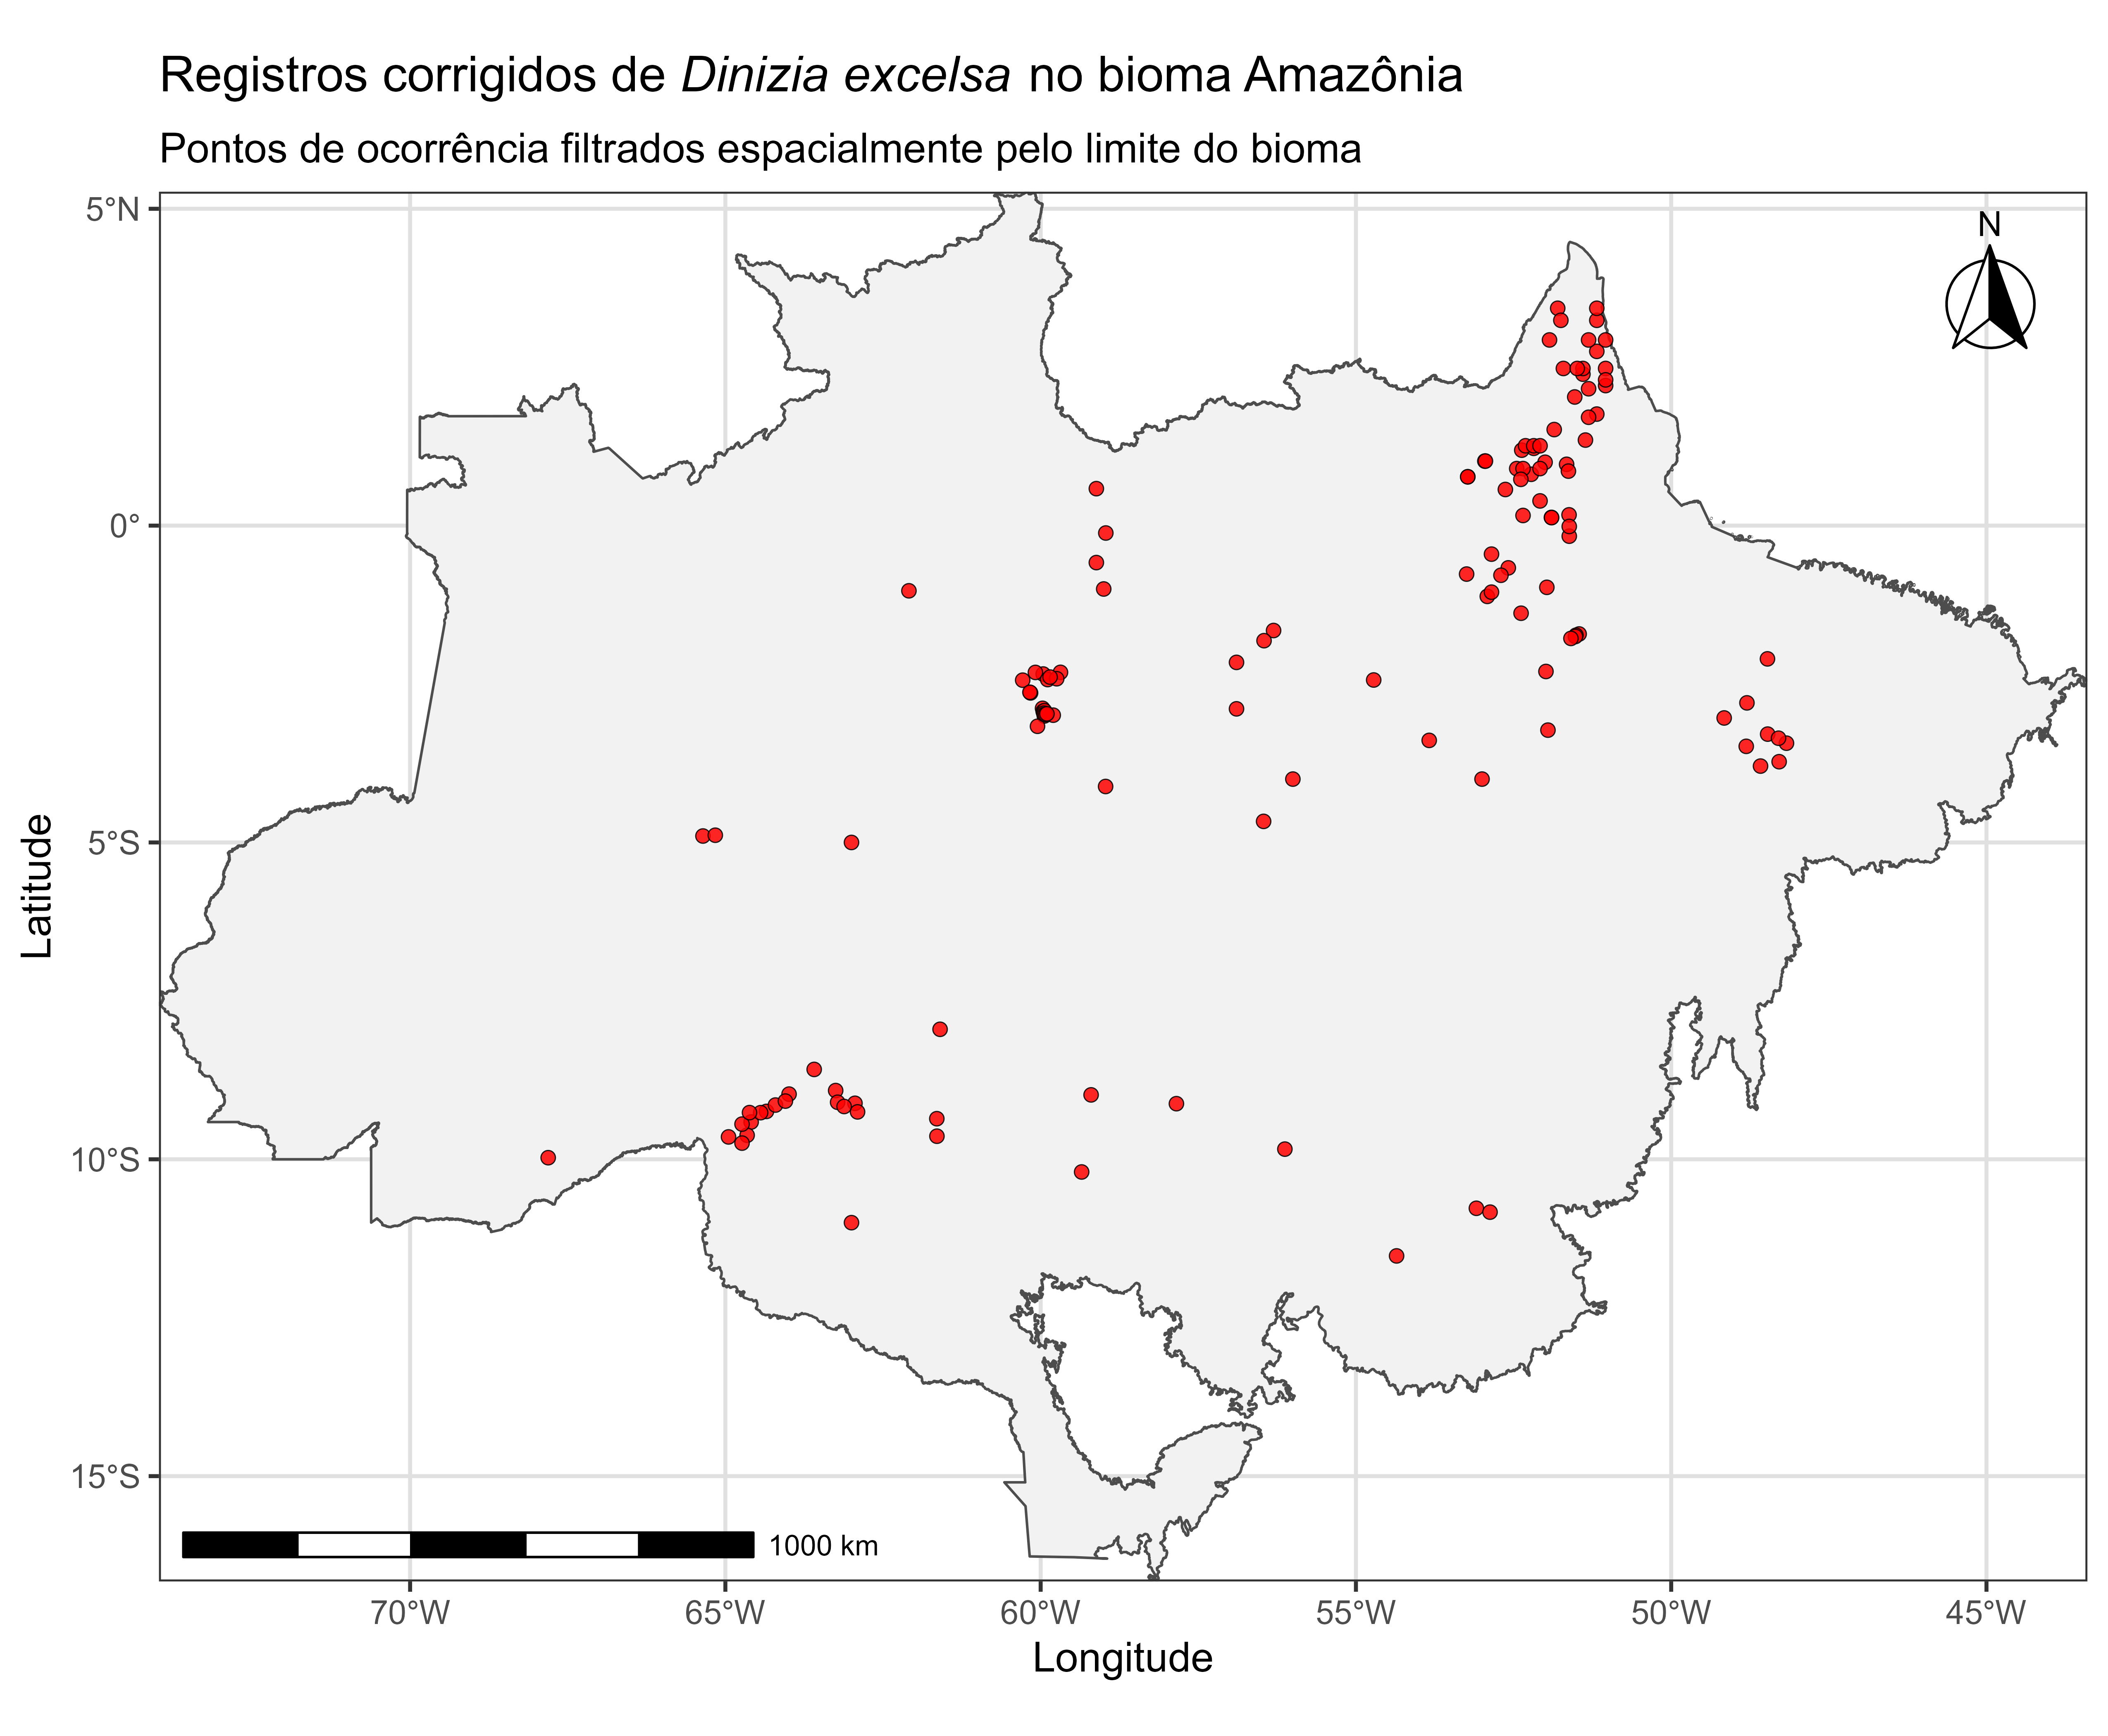
\includegraphics[width=0.90\textwidth]
	{figuras/unidade01/unidade01_mapa_ocorrencias_dinizia.png}
	\caption{
		Distribuição observada de \textit{Dinizia excelsa} no bioma Amazônia após os procedimentos de limpeza e filtragem espacial dos dados de ocorrência. Os pontos representam registros utilizados nas análises desta unidade.
	}
	\label{fig:unidade01_ocorrencias_dinizia}
\end{figure}

Observa-se que a espécie apresenta distribuição predominantemente associada ao domínio amazônico, com registros concentrados principalmente nas regiões de floresta tropical úmida. Entretanto, como discutido anteriormente, esses registros representam apenas a distribuição observada da espécie e não necessariamente sua distribuição real ou potencial.

A simples visualização dos pontos de ocorrência não permite compreender quais fatores ambientais explicam esse padrão espacial. Para responder essa questão é necessário deslocar a análise do espaço geográfico para o espaço ambiental.

\subsection{As condições ambientais associadas à espécie}

Segundo a perspectiva grinnelliana do nicho ecológico, a distribuição das espécies é fortemente influenciada pelas condições ambientais necessárias para sua sobrevivência e persistência.

Para investigar essas relações, foram utilizadas quatro variáveis bioclimáticas amplamente empregadas em estudos ecológicos:

\begin{itemize}
	
	\item BIO1 -- Temperatura média anual;
	
	\item BIO4 -- Sazonalidade da temperatura;
	
	\item BIO12 -- Precipitação anual;
	
	\item BIO15 -- Sazonalidade da precipitação.
	
\end{itemize}

Essas variáveis representam importantes gradientes climáticos capazes de influenciar processos fisiológicos, crescimento, recrutamento, mortalidade e produtividade das árvores tropicais \parencite{malhi2009,esquivel2020}.

A Figura~\ref{fig:unidade01_variaveis_patchwork} apresenta a distribuição espacial dessas variáveis no bioma Amazônia juntamente com os registros de ocorrência de \textit{Dinizia excelsa}.

\begin{figure}[H]
	\centering
	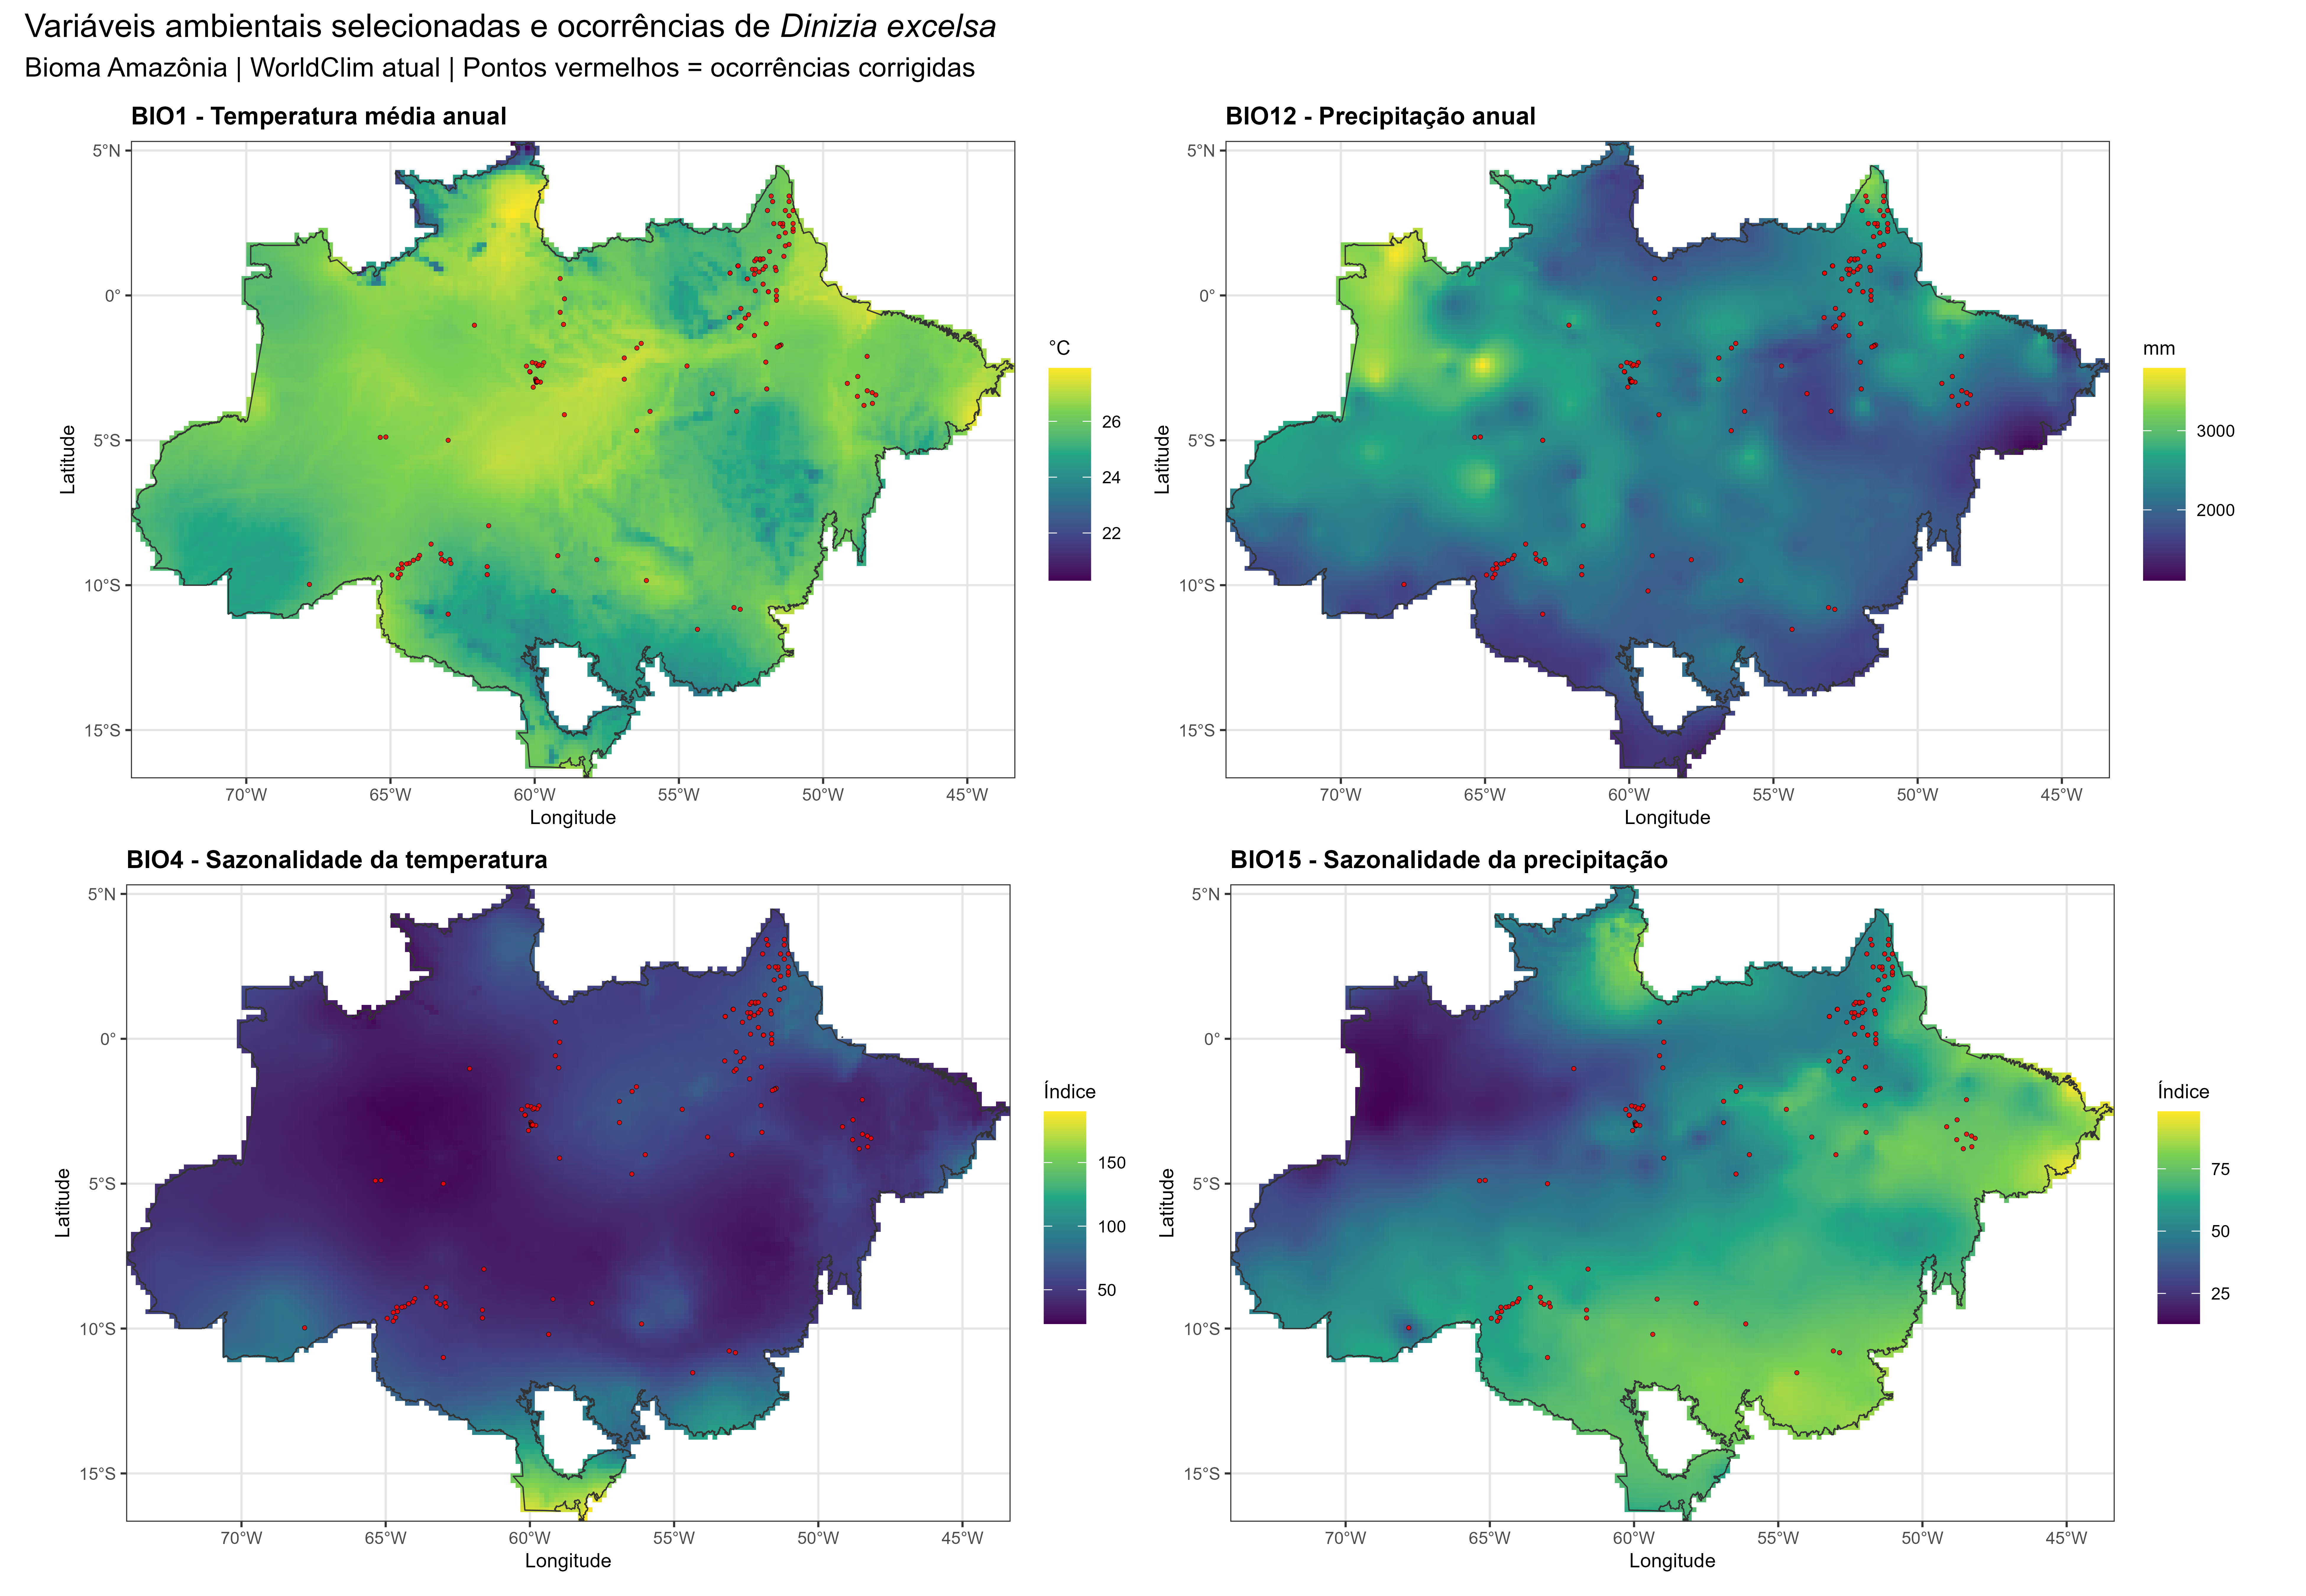
\includegraphics[width=\textwidth]
	{figuras/unidade01/unidade01_mapas_variaveis_patchwork_dinizia.png}
	\caption{
		Gradientes climáticos representados pelas variáveis BIO1, BIO4, BIO12 e BIO15 e sua relação com as ocorrências de \textit{Dinizia excelsa} na Amazônia.
	}
	\label{fig:unidade01_variaveis_patchwork}
\end{figure}

Os mapas revelam que a espécie não ocorre aleatoriamente ao longo dos gradientes ambientais disponíveis. Pelo contrário, os registros concentram-se em determinadas combinações de temperatura e precipitação, sugerindo a existência de restrições ambientais associadas ao nicho climático da espécie.

Esse padrão ilustra diretamente o conceito de filtro ambiental discutido anteriormente. Embora grande parte da Amazônia apresente clima favorável ao desenvolvimento de florestas tropicais, apenas uma fração desse espaço ambiental é efetivamente ocupada pela espécie.

\subsection{Visualizando o nicho climático no espaço ambiental}

Uma das contribuições centrais de Hutchinson foi demonstrar que o nicho ecológico deve ser compreendido no espaço ambiental e não apenas no espaço geográfico.

Para visualizar essa ideia, a Figura~\ref{fig:unidade01_nicho_tp_dinizia} representa as ocorrências de \textit{Dinizia excelsa} em um espaço climático definido por temperatura média anual e precipitação anual.

\begin{figure}[H]
	\centering
	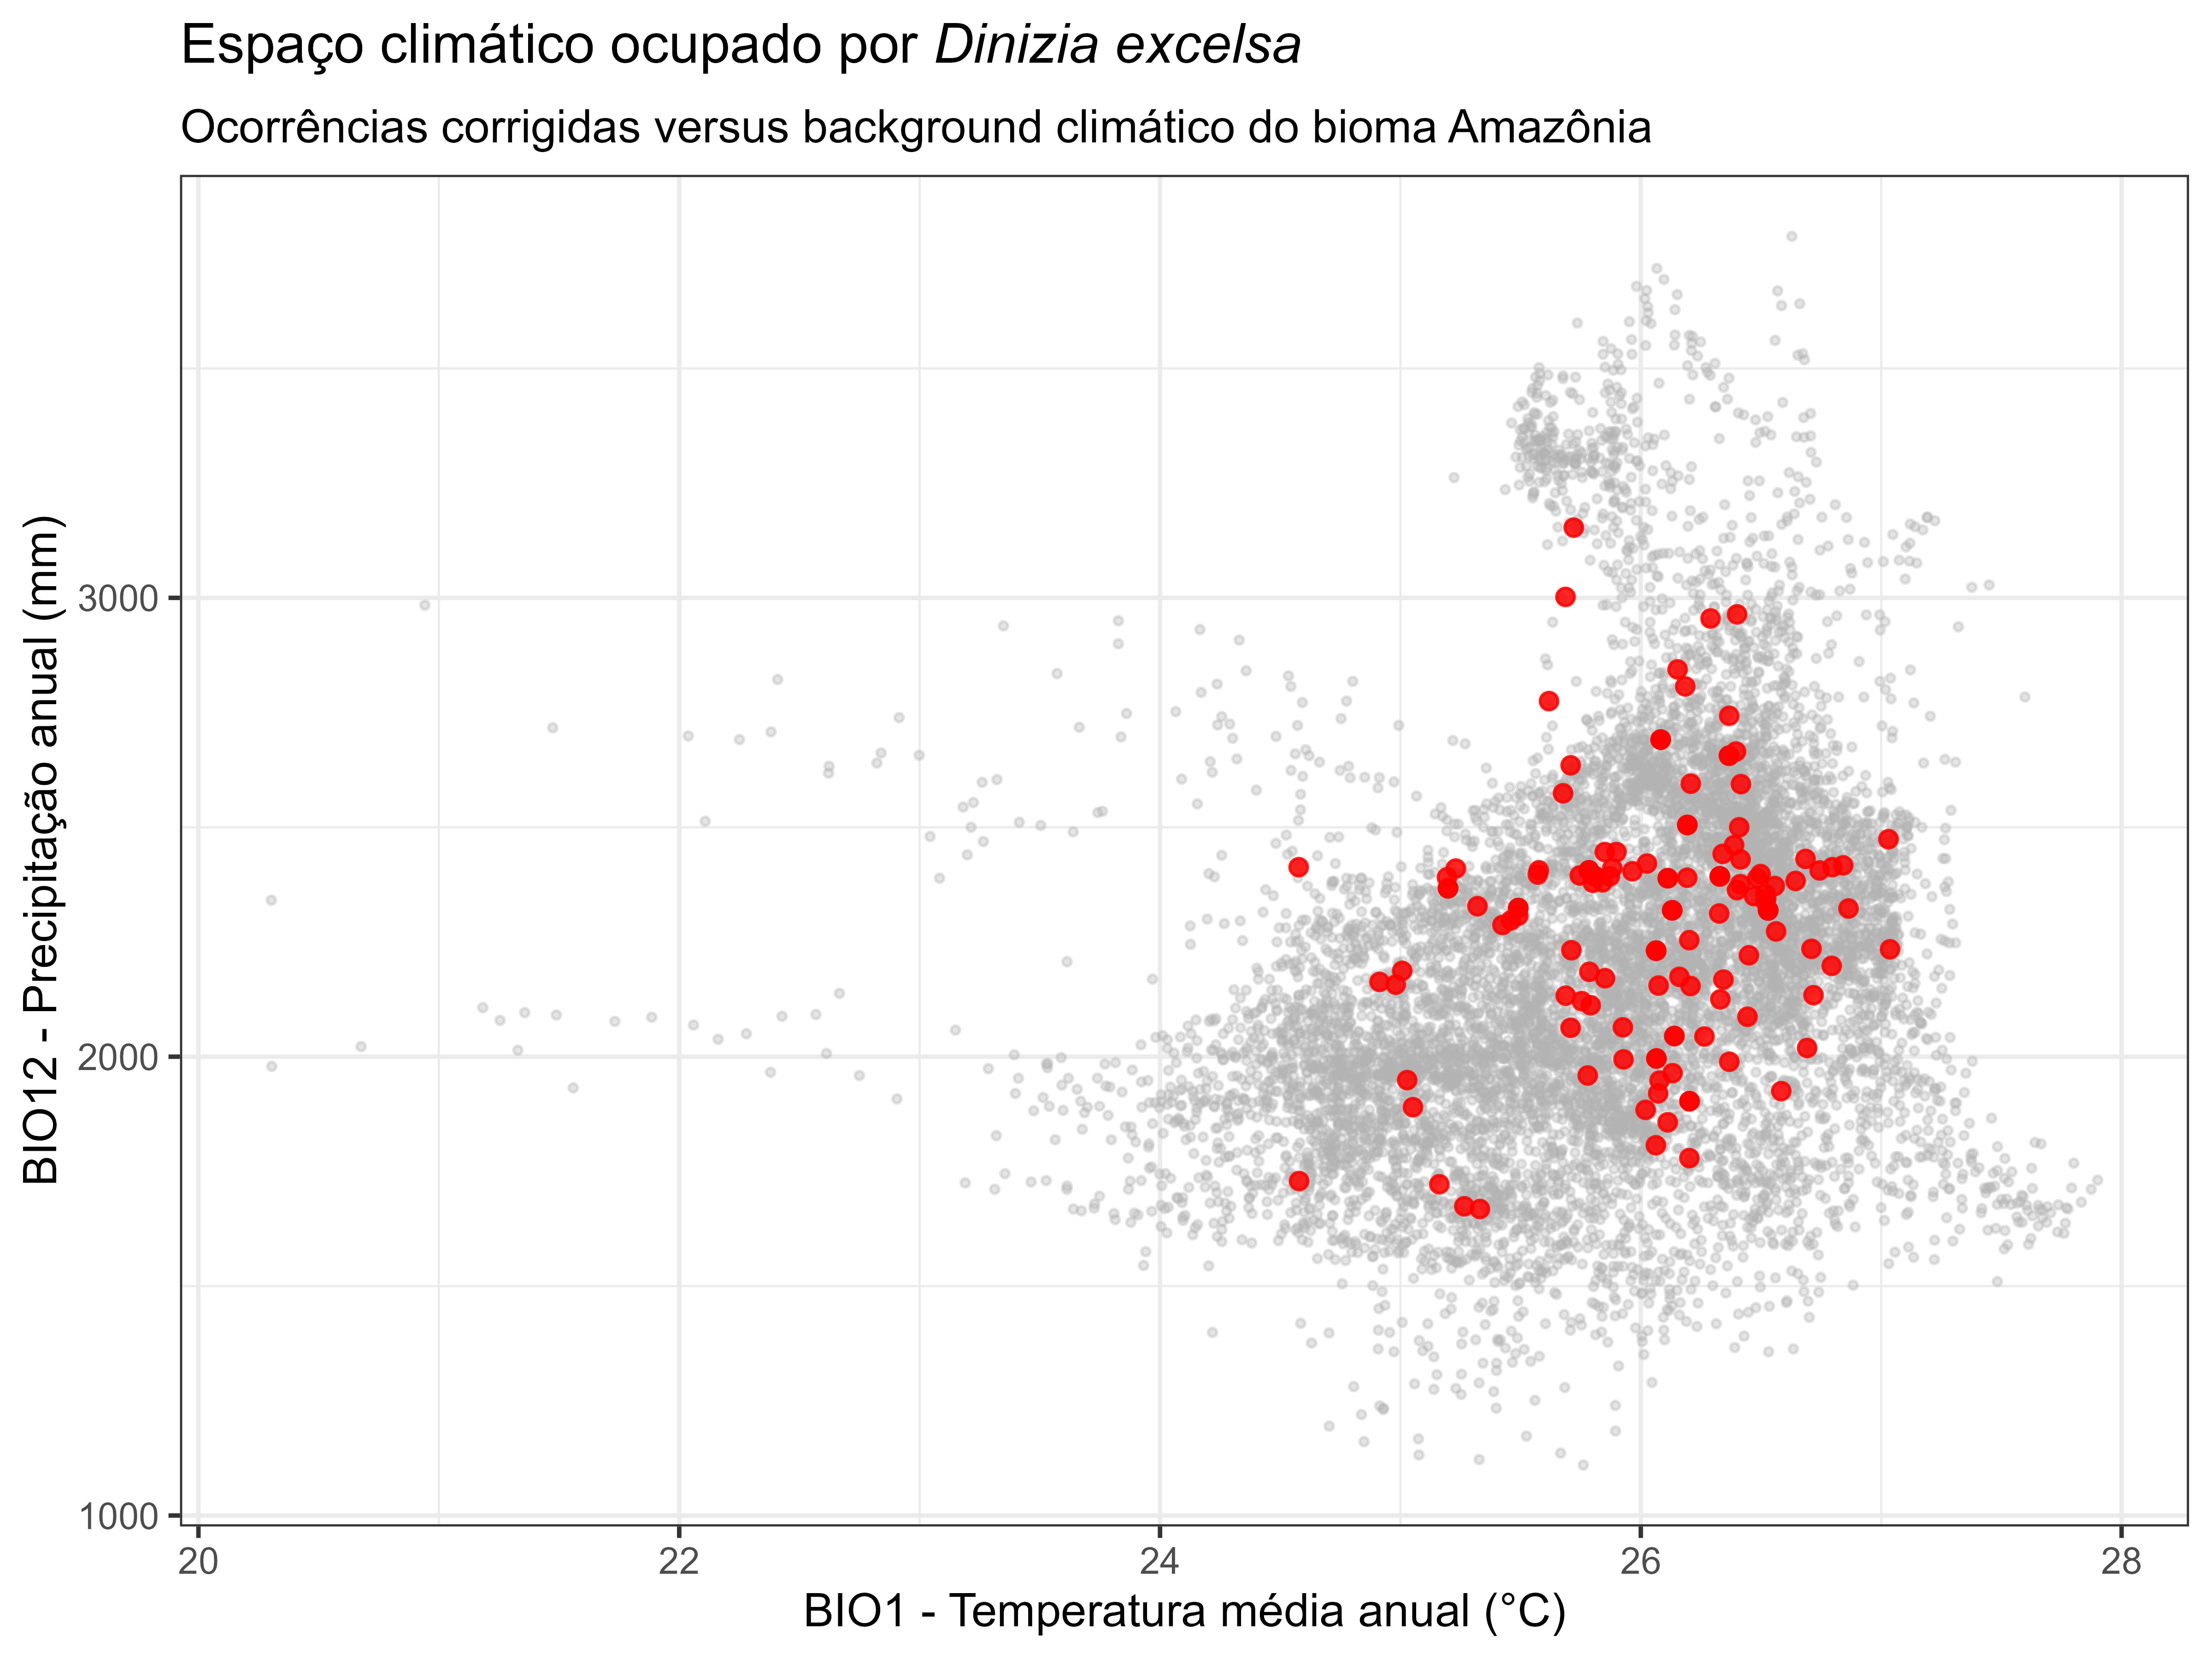
\includegraphics[width=0.85\textwidth]
	{figuras/unidade01/unidade01_nicho_temperatura_precipitacao_dinizia.png}
	\caption{
		Espaço climático ocupado por \textit{Dinizia excelsa}. Os pontos cinza representam o ambiente disponível na Amazônia e os pontos vermelhos representam as condições climáticas associadas às ocorrências da espécie.
	}
	\label{fig:unidade01_nicho_tp_dinizia}
\end{figure}

Observa-se que os registros da espécie ocupam apenas uma fração do conjunto de condições ambientais disponíveis no bioma Amazônia. Isso significa que a espécie não utiliza todo o ambiente climático disponível, mas apenas determinadas combinações ambientais compatíveis com seu nicho ecológico.

Essa observação fornece uma evidência empírica da diferença entre ambiente disponível e ambiente utilizado, um dos princípios centrais da teoria moderna do nicho ecológico.

Além disso, evidencia que a simples existência de condições ambientais adequadas não garante a ocupação da área, reforçando a importância dos componentes bióticos e de acessibilidade discutidos no framework BAM.

\subsection{Uma visão multivariada do nicho ecológico}

Embora gráficos bidimensionais sejam úteis para fins didáticos, o nicho ecológico é inerentemente multidimensional.

Na prática, espécies respondem simultaneamente a diversos fatores ambientais. Por essa razão, técnicas multivariadas frequentemente são utilizadas para explorar a estrutura do espaço ambiental.

A Figura~\ref{fig:unidade01_pca_nicho} apresenta uma representação do nicho climático de \textit{Dinizia excelsa} utilizando Análise de Componentes Principais (PCA).

\begin{figure}[H]
	\centering
	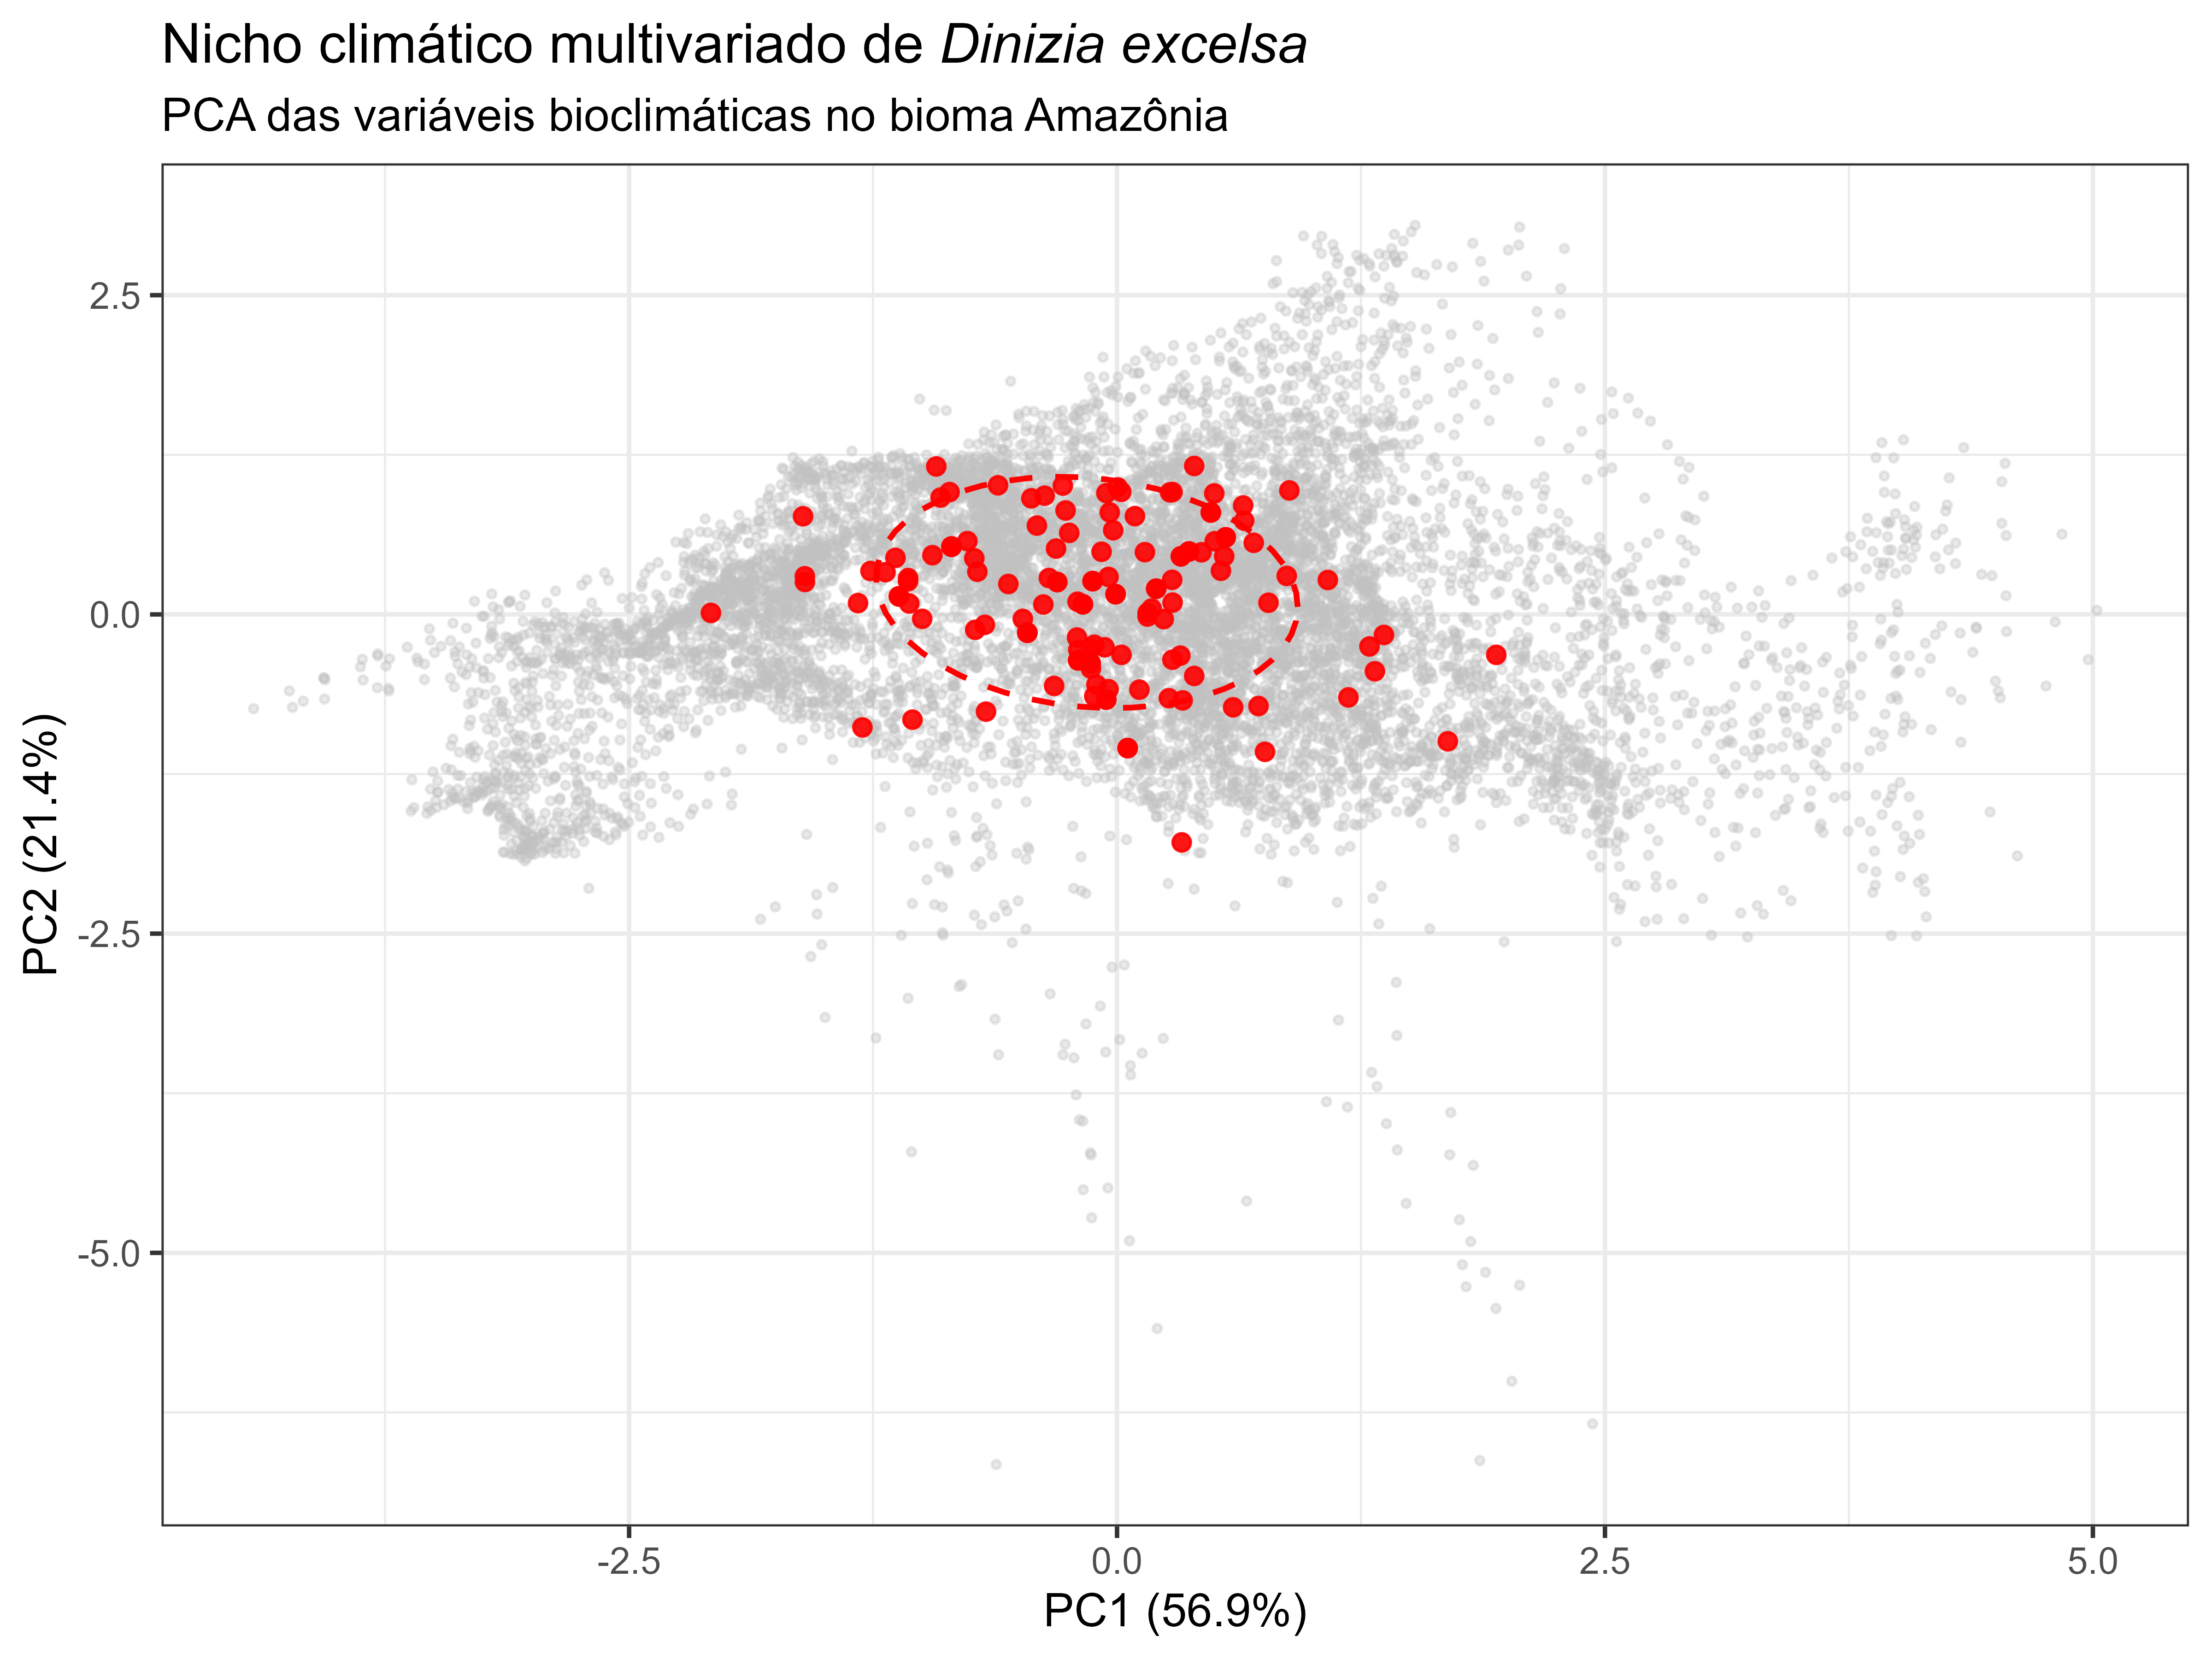
\includegraphics[width=0.85\textwidth]
	{figuras/unidade01/unidade01_pca_nicho_climatico_dinizia.png}
	\caption{
		Representação do nicho climático de \textit{Dinizia excelsa} no espaço ambiental multivariado utilizando Análise de Componentes Principais (PCA).
	}
	\label{fig:unidade01_pca_nicho}
\end{figure}

Nesse gráfico, os pontos cinza representam o conjunto de condições climáticas disponíveis na Amazônia, enquanto os pontos associados à espécie representam o subconjunto efetivamente ocupado.

Essa representação aproxima-se da ideia de hipervolume ecológico proposta por Hutchinson. Embora a PCA reduza a dimensionalidade dos dados, ela permite visualizar como a espécie ocupa apenas uma parcela específica do espaço ambiental disponível.

Em termos ecológicos, isso significa que a distribuição observada da espécie resulta da combinação de filtros ambientais, limitações históricas de dispersão e interações ecológicas que restringem sua ocupação ao longo da paisagem amazônica.

\subsection{Conectando teoria e modelagem}

Este estudo de caso demonstra como os conceitos apresentados ao longo desta unidade convergem para formar a base teórica da Modelagem de Distribuição de Espécies.

A distribuição observada de \textit{Dinizia excelsa} representa a manifestação geográfica de um conjunto complexo de processos ecológicos. Os registros de ocorrência permitem inferir parte do nicho realizado da espécie. As variáveis ambientais representam aproximações dos componentes abióticos do nicho. O espaço ambiental permite visualizar as condições utilizadas pela espécie. O framework BAM fornece uma explicação integrada para a distribuição observada. E a hipótese de conservação de nicho permite utilizar essas relações para projeções espaciais e temporais.

Em outras palavras, a Modelagem de Distribuição de Espécies pode ser entendida como uma tentativa quantitativa de representar, em linguagem matemática e espacial, os princípios ecológicos discutidos ao longo desta unidade.

\subsection{Do nicho ecológico à Modelagem de Distribuição de Espécies}

Nas próximas unidades, o leitor aprenderá a transformar esses conceitos em procedimentos analíticos reproduzíveis utilizando o software R.

Serão abordados os métodos para obtenção de dados de ocorrência, preparação de variáveis ambientais, delimitação da área acessível ((M)), avaliação de multicolinearidade, calibração de modelos e projeções sob diferentes cenários ambientais.

Assim, o estudo de caso apresentado nesta seção funciona como uma ponte entre os fundamentos ecológicos discutidos nesta unidade e as etapas práticas de modelagem que serão desenvolvidas ao longo do restante do livro.

\begin{importantbox}
	
	\textbf{Reprodutibilidade científica}
	
	Todas as figuras apresentadas neste estudo de caso foram geradas utilizando dados reais de ocorrência de \textit{Dinizia excelsa}, variáveis bioclimáticas do WorldClim e rotinas desenvolvidas em linguagem R.
	
	Os scripts completos utilizados para obtenção dos dados, limpeza das ocorrências, extração das variáveis ambientais, construção dos gráficos e geração das análises encontram-se disponíveis nos apêndices deste livro e no repositório oficial do projeto.
	
	Essa abordagem garante transparência, reprodutibilidade e permite que o leitor reproduza integralmente todas as análises apresentadas.
	
\end{importantbox}

A partir deste ponto, o leitor já possui os fundamentos ecológicos necessários para compreender como os modelos de distribuição são construídos e interpretados. Nas próximas unidades iniciaremos a transição da teoria ecológica para a implementação prática da Modelagem de Distribuição de Espécies em R.

%================================================
\section{Síntese conceitual da unidade}
%================================================

Ao longo desta unidade foram apresentados os fundamentos ecológicos que sustentam a Modelagem de Distribuição de Espécies. Embora os modelos modernos utilizem algoritmos sofisticados e grandes volumes de dados ambientais, sua interpretação permanece fortemente dependente dos conceitos desenvolvidos pela Ecologia ao longo do último século.

A discussão iniciou-se com a compreensão da distribuição das espécies como um dos problemas centrais da Ecologia e da Biogeografia. Desde os trabalhos pioneiros de Darwin, Wallace e Humboldt, pesquisadores buscam compreender por que determinadas espécies ocorrem em algumas regiões e estão ausentes de outras. Essa questão permanece no centro da Modelagem de Distribuição de Espécies e motiva grande parte das aplicações contemporâneas em conservação da biodiversidade, mudanças climáticas e planejamento ambiental.

Em seguida, foi apresentada a evolução histórica do conceito de nicho ecológico. A perspectiva de Grinnell destacou a importância dos fatores ambientais na determinação da distribuição das espécies. Posteriormente, Elton ampliou essa visão ao incorporar as interações ecológicas e o papel funcional dos organismos nas comunidades biológicas. Finalmente, Hutchinson formalizou o nicho como um hipervolume multidimensional definido por múltiplos gradientes ambientais e ecológicos, estabelecendo a base conceitual da moderna Modelagem de Distribuição de Espécies.

A partir da formulação de Hutchinson, foram discutidos os conceitos de nicho fundamental e nicho realizado. O nicho fundamental representa o conjunto de condições ambientais compatíveis com a persistência da espécie, enquanto o nicho realizado corresponde à parcela desse potencial efetivamente ocupada após a ação de interações ecológicas, limitações de dispersão e processos históricos. Essa distinção é fundamental para compreender o que os modelos de distribuição realmente estimam quando utilizam registros de ocorrência para inferir padrões ecológicos.

Também foi apresentada a diferença entre espaço geográfico e espaço ambiental. Enquanto o primeiro descreve onde as espécies ocorrem, o segundo descreve sob quais condições ambientais elas ocorrem. Essa distinção constitui o núcleo conceitual da SDM moderna, pois os modelos aprendem relações no espaço ambiental e posteriormente projetam essas relações para o espaço geográfico.

O framework BAM forneceu uma estrutura integradora para compreender a distribuição das espécies como resultado da interação entre fatores abióticos ((A)), fatores bióticos ((B)) e acessibilidade ou dispersão ((M)). Essa abordagem demonstra que a simples existência de condições ambientais adequadas não garante a ocorrência de uma espécie, uma vez que processos históricos, ecológicos e biogeográficos também influenciam a distribuição observada.

Posteriormente, foram discutidas as diferenças entre distribuição observada, distribuição real e distribuição potencial. Enquanto a distribuição observada corresponde aos registros disponíveis, a distribuição real representa a ocupação efetiva da espécie na natureza e a distribuição potencial corresponde às áreas ambientalmente adequadas inferidas pelos modelos. Essa distinção é essencial para interpretar corretamente mapas de adequabilidade ambiental.

A unidade também abordou a hipótese de conservação de nicho, um dos pressupostos centrais das projeções espaciais e temporais realizadas em SDM. A possibilidade de transferir modelos para cenários futuros, paleoclimáticos ou regiões distintas depende da estabilidade relativa das relações espécie--ambiente ao longo do tempo e do espaço.

Por fim, o estudo de caso utilizando \textit{Dinizia excelsa} demonstrou como esses conceitos podem ser integrados em uma aplicação prática. A análise das ocorrências da espécie e sua relação com gradientes climáticos da Amazônia permitiu visualizar, de forma concreta, a transição entre espaço geográfico, espaço ambiental e nicho ecológico.

Em síntese, a Modelagem de Distribuição de Espécies pode ser entendida como uma tentativa quantitativa de representar, em linguagem matemática e espacial, as relações ecológicas que conectam organismos, ambiente e distribuição geográfica. Compreender esses fundamentos é indispensável para interpretar adequadamente os modelos que serão desenvolvidos nas unidades seguintes.

%================================================
\section{Leituras essenciais}
%================================================

Os trabalhos listados a seguir representam algumas das referências mais importantes para aprofundamento dos conceitos discutidos nesta unidade. Recomenda-se que o leitor consulte essas obras ao longo do desenvolvimento do livro, pois muitos dos conceitos apresentados nas próximas unidades derivam diretamente dessas contribuições.

\subsection*{Ecologia e Nicho Ecológico}

\begin{itemize}
	
	\item Grinnell, J. (1917). \textit{The niche-relationships of the California Thrasher}. Auk, 34, 427--433.
	
	\item Elton, C. S. (1927). \textit{Animal Ecology}. London: Sidgwick & Jackson.
	
	\item Hutchinson, G. E. (1957). \textit{Concluding Remarks}. Cold Spring Harbor Symposia on Quantitative Biology, 22, 415--427.
	
	\item Begon, M., Townsend, C. R., & Harper, J. L. (2006). \textit{Ecology: From Individuals to Ecosystems}. Blackwell Publishing.
	
	\item Ricklefs, R. E. (2010). \textit{A Economia da Natureza}. Guanabara Koogan.
	
\end{itemize}

\subsection*{Biogeografia e Distribuição das Espécies}

\begin{itemize}
	
	\item Brown, J. H., Lomolino, M. V. (1998). \textit{Biogeography}. Sinauer Associates.
	
	\item Gaston, K. J. (2003). \textit{The Structure and Dynamics of Geographic Ranges}. Oxford University Press.
	
	\item Wiens, J. J., Graham, C. H. (2005). Niche conservatism. \textit{Annual Review of Ecology, Evolution and Systematics}, 36, 519--539.
	
\end{itemize}

\subsection*{Modelagem de Distribuição de Espécies}

\begin{itemize}
	
	\item Franklin, J. (2010). \textit{Mapping Species Distributions: Spatial Inference and Prediction}. Cambridge University Press.
	
	\item Peterson, A. T., Soberón, J., Pearson, R. G., et al. (2011). \textit{Ecological Niches and Geographic Distributions}. Princeton University Press.
	
	\item Guisan, A., Thuiller, W., Zimmermann, N. E. (2017). \textit{Habitat Suitability and Distribution Models}. Cambridge University Press.
	
	\item Elith, J., Leathwick, J. R. (2009). Species Distribution Models: Ecological Explanation and Prediction Across Space and Time. \textit{Annual Review of Ecology, Evolution and Systematics}, 40, 677--697.
	
	\item Soberón, J. (2007). Grinnellian and Eltonian niches and geographic distributions of species. \textit{Ecology Letters}, 10, 1115--1123.
	
\end{itemize}

\subsection*{Mudanças Climáticas e Conservação}

\begin{itemize}
	
	\item Araújo, M. B., Peterson, A. T. (2012). Uses and misuses of bioclimatic envelope modeling. \textit{Ecology}, 93, 1527--1539.
	
	\item Thuiller, W., Lavorel, S., Araújo, M. B., et al. (2005). Climate change threats to plant diversity in Europe. \textit{PNAS}, 102, 8245--8250.
	
	\item IPCC (2021). \textit{Climate Change 2021: The Physical Science Basis}. Cambridge University Press.
	
\end{itemize}

%================================================
\begin{exercicios}
	%================================================
	
	\begin{enumerate}
		
		\item Explique por que a distribuição geográfica das espécies é considerada um dos problemas centrais da Ecologia e da Biogeografia.
		
		\item Compare as interpretações de nicho propostas por Grinnell, Elton e Hutchinson. Quais são as principais diferenças entre essas abordagens e como elas contribuíram para a construção da moderna Modelagem de Distribuição de Espécies?
		
		\item Diferencie nicho fundamental e nicho realizado. Forneça exemplos ecológicos que ilustrem como uma espécie pode ocupar apenas parte de seu nicho potencial.
		
		\item Explique a diferença entre espaço geográfico e espaço ambiental. Por que essa distinção é fundamental para compreender o funcionamento dos algoritmos de SDM?
		
		\item Utilizando o framework BAM, descreva como fatores abióticos, fatores bióticos e limitações de dispersão podem influenciar simultaneamente a distribuição de uma espécie.
		
		\item Diferencie distribuição observada, distribuição real e distribuição potencial. Quais são as implicações dessas diferenças para a interpretação de mapas de adequabilidade ambiental?
		
		\item Explique o conceito de conservação de nicho. Por que esse conceito é essencial para projeções de distribuição futura sob cenários de mudanças climáticas?
		
		\item Discuta as principais limitações associadas à utilização de modelos de distribuição para prever respostas das espécies às mudanças climáticas globais.
		
		\item Com base no estudo de caso apresentado para \textit{Dinizia excelsa}, explique como os registros de ocorrência podem ser utilizados para inferir relações entre espécies e ambiente.
		
		\item Considere uma espécie amazônica cuja distribuição atual esteja associada a regiões com elevada precipitação anual. Descreva como mudanças climáticas que reduzam a disponibilidade hídrica poderiam afetar sua distribuição potencial. Quais fatores ecológicos adicionais deveriam ser considerados para interpretar corretamente os resultados do modelo?
		
	\end{enumerate}
	
%================================================
\end{exercicios}
%================================================
